\documentclass{article}

\usepackage[utf8]{inputenc}
\usepackage[spanish]{babel}
\usepackage{geometry}
\usepackage{graphicx}
\usepackage{titlesec}
\usepackage{lipsum}
\usepackage[dvipsnames]{xcolor}
\usepackage[fleqn]{mathtools}
\usepackage{booktabs}
\usepackage{amsmath}
\usepackage{latexsym}
\usepackage{nccmath}
\usepackage{multicol}
\usepackage{listings}
\usepackage{tasks}
\usepackage{color}
\usepackage{float}
\usepackage{enumitem}
\usepackage{longtable}
\usepackage{makecell}
\usepackage{caption}
\usepackage[parfill]{parskip}
\usepackage{lipsum}
\usepackage{enumitem}
\usepackage{hyperref}% Para manejar enlaces
\usepackage{fancyhdr}
\usepackage{adjustbox}
\usepackage{amsmath}
\usepackage{tocloft}
\usepackage{soul}
\babelprovide[import=es]{nil}
%Definicion de colores
\definecolor{colorIPN}{rgb}{0.5, 0.0,0.13}
\definecolor{colorESCOM}{rgb}{0.0, 0.5,1.0}
\definecolor{myorange}{RGB}{255, 204, 153}
\graphicspath{ {imagenes/} }
%Configuraciones extras de colores
\definecolor{codegreen}{rgb}{0,0.6,0}
\definecolor{codered}{rgb}{0.6,0,0}
\definecolor{codegray}{rgb}{0.5,0.5,0.5}
\definecolor{codepurple}{rgb}{0.58,0,0.82}
\definecolor{backcolour}{rgb}{0.95,0.95,0.92}

% Configuración de la portada
\titleformat{\section}[block]{\normalfont\huge\bfseries}{\thesection}{1em}{}
\geometry{a4paper, margin=1in}

% Definir comandos para información repetitiva
\newcommand{\logoInstitucion}{logotipo_ipn.png} % Reemplaza con el nombre del archivo de tu logo
\newcommand{\logoUniversidad}{EscudoESCOM.png} % Reemplaza con el nombre del archivo de tu logo
\newcommand{\nombreInstituto}{Instituto Politecnico Nacional}
\newcommand{\facultad}{Escuela Superior de Computo}
\newcommand{\materia}{Teoría de la Computación}
\newcommand{\grupo}{5BM1}
\newcommand{\profesora}{Genaro Juarez Martínez}
\newcommand{\periodo}{2024/02}
\newcommand{\alumno}{Carrillo Barreiro José Emiliano}

% Definir nuevas listas para información repetitiva
\newlist{bracketed}{enumerate}{1}
\setlist[bracketed,1]{label={[{\arabic*}]},left=0pt}

% Configuración del encabezado y pie de página
\pagestyle{fancy}
\fancyhf{} % Limpia todos los campos

% Encabezado
\fancyhead[C]{\textbf{\nombreInstituto\\ \facultad}}
\fancyhead[L]{
\includegraphics[width=1cm]{logotipo_ipn.png}}
\fancyhead[R]{
\includegraphics[width=1.5cm]{EscudoESCOM.png}}

% Pie de página
\fancyfoot[C]{\materia||\grupo\\ \alumno\\ \thepage}

% Configuración del grosor de la línea en el encabezado y pie de página
\renewcommand{\headrulewidth}{0.4pt}
\renewcommand{\footrulewidth}{0.4pt}

% Ajuste del tamaño del encabezado
\setlength{\headheight}{34.0845pt}
\addtolength{\topmargin}{-22.0845pt}

% Configuración de lstlisting para Python
\lstdefinestyle{mystyle}{
    backgroundcolor=\color{backcolour},
    commentstyle=\color{codegreen},
    keywordstyle=\color{codepurple},
    numberstyle=\tiny\color{codegray},
    stringstyle=\color{codered},
    basicstyle=\ttfamily\small,
    breakatwhitespace=false,
    breaklines=true,
    captionpos=b,
    keepspaces=true,
    numbers=left,
    numbersep=5pt,
    showspaces=false,
    showstringspaces=false,
    showtabs=false,
    tabsize=2
}

\lstdefinestyle{custompython}{
    language=Python,
    basicstyle=\small\ttfamily,
    keywordstyle=\color{blue},
    stringstyle=\color{green},
    commentstyle=\color{red},
    numbers=left,
    numberstyle=\tiny\color{gray},
    stepnumber=1,
    numbersep=5pt,
    backgroundcolor=\color{white},
    frame=single,
    captionpos=b,
    breaklines=true,
    breakatwhitespace=false,
    showstringspaces=false,
    morekeywords={import,plt,np,ws,y,gradient}
}

% Definición de estilo para C++
\lstdefinestyle{cppstyle}{
    language=C++,
    basicstyle=\small\ttfamily,
    keywordstyle=\color{blue},
    commentstyle=\color{green!40!black},
    stringstyle=\color{orange},
    showstringspaces=false,
    breaklines=true,
    breakatwhitespace=true,
    numbers=left,
    numberstyle=\tiny,
    stepnumber=1,
    numbersep=5pt,
    frame=single,
    captionpos=b,
    backgroundcolor=\color{gray!5},
    xleftmargin=0.5cm,
    xrightmargin=0.5cm
}

% Definición de estilo para MATLAB
\lstdefinestyle{matlabstyle}{
    language=Matlab,
    basicstyle=\small\ttfamily,
    keywordstyle=\color{blue},
    commentstyle=\color{green!40!black},
    stringstyle=\color{purple!50!blue!50!white},
    showstringspaces=false,
    breaklines=true,
    breakatwhitespace=true,
    numbers=left,
    numberstyle=\tiny,
    stepnumber=1,
    numbersep=5pt,
    frame=single,
    captionpos=b,
    backgroundcolor=\color{gray!5},
    xleftmargin=0.5cm,
    xrightmargin=0.5cm
}

% Personalización del índice de listados
\newcommand{\listcppname}{Índice de Listados de C++}
\newcommand{\listmatlabname}{Índice de Listados de MATLAB}
\newlistof{cpplistings}{lolcpp}{\listcppname}
\newlistof{matlablistings}{lolmatlab}{\listmatlabname}

% Configuración para los listados de C++
\lstset{style=cppstyle}
\newcommand{\cpplisting}[1]{%
    \refstepcounter{cpplistings}%
    \addcontentsline{lolcpp}{cpplistings}{\protect\numberline{\thecpplistings}#1}\par}

% Configuración para los listados de MATLAB
\lstset{style=matlabstyle}
\newcommand{\matlablisting}[1]{%
    \refstepcounter{matlablistings}%
    \addcontentsline{lolmatlab}{matlablistings}{\protect\numberline{\thematlablistings}#1}\par}

\begin{document}

% Portada
\begin{titlepage}
    \begin{center}
        \vspace*{1cm}

        \includegraphics[width=0.25\textwidth]{\logoInstitucion}

        \vspace{1cm}

        \textbf{\LARGE \nombreInstituto} \\
        \textbf{\Large \facultad} \\
        \vspace{0.5cm}
        \textbf{\large Materia: \materia} \\
        \textbf{\large Grupo: \grupo} \\
        \vspace{0.5cm}
        \textbf{\large Profesor: \profesora} \\
        \textbf{\large Periodo: \periodo} \\

        \vspace{1cm}

        \textbf{\LARGE Bloque de programas 01:} \\
        \vspace{0.5cm}
        \textbf{\Large Generador de potencias: de un alfabeto binario, de rutas ganadoras en un tablro de ajedrez; y buscador de palabras.} \\

        \vfill

        \textbf{\large Realizado por:} \\
        \textbf{\large \alumno}

        \vspace{1cm}

        \includegraphics[width=0.4\textwidth]{\logoUniversidad}

        \vspace{1cm}

        \textbf{\large \facultad} \\
        \textbf{\large Fecha: \today}

    \end{center}
\end{titlepage}

% Índice
\tableofcontents
\newpage
\listofcpplistings%Crea indice de codigos en C++
\listofmatlablistings%Crea indice de codigos en MATLAB
%\listoftables
\listoffigures
\listoftables
\newpage

\section{Resumen.}
El presente informe detalla el desarrollo de tres programas en el contexto de la teoría de autómatas y la programación interactiva. Cada programa aborda distintos aspectos y funcionalidades, con el objetivo común de ejecutarse de manera automática y permitir la interacción manual según las necesidades del usuario.

El primer programa, \textit{Universo de Cadenas Binarias}, se enfoca en la generación y manipulación de cadenas binarias de longitud
variable. Permite al usuario o al programa determinar la longitud de las cadenas, generando la salida en formato de conjunto y
guardándola en un archivo de texto. Además, se realiza un análisis detallado para una longitud específica, incluyendo cálculos y
gráficos.

El segundo programa, \textit{Tablero de Ajedrez}, simula el movimiento de piezas en un tablero de $4*4$, con la posibilidad de
movimientos ortogonales y diagonales. Implementa un juego para dos jugadores, generando rutas de movimiento y detectando posibles
movimientos ganadores. Se ofrece la opción de juego automático o manual, con la posibilidad de introducir o generar aleatoriamente la
cadena de movimientos.

El tercer programa, \textit{Buscador de Palabras}, desarrolla un autómata que reconoce un conjunto específico de palabras. Se diseña y
transforma un NFA a DFA, permitiendo la lectura de un archivo de texto o página web para identificar las palabras reservadas y contar
su ocurrencia. Se genera un archivo que registra la evaluación del autómata por cada carácter leído, y se grafica el DFA resultante.

Cada programa se acompaña de su respectivo código fuente en LaTeX, proporcionando una visión detallada de la implementación.
El informe final se presenta en un único PDF que recopila todos los detalles de los programas, sus funcionalidades y los resultados
obtenidos durante su ejecución.


\section{Introducción.}
En el presente informe se detallan las actividades realizadas en el marco de un proyecto que engloba tres programas distintos,
cada uno abordando diferentes aspectos de la teoría de autómatas y la programación de sistemas interactivos. Estos programas han
sido desarrollados con el objetivo de ejecutarse de manera automática, permitiendo al usuario interactuar con ellos de forma manual
según sea necesario. A continuación, se presenta un resumen de cada programa junto con sus características principales:

\subsection*{Programa 1: Universo de Cadenas Binarias}
En este programa se aborda la generación y manipulación del universo de cadenas binarias de longitud variable, representadas por el
conjunto $\Sigma^n$. Se permite al usuario o al programa determinar el valor de $n$, con un rango válido entre 0 y 1000. El programa
puede ejecutarse tanto en modo automático como manual, generando la salida en formato de conjunto y guardándola en un archivo de texto. Además, se realiza un análisis específico para $n=28$, incluyendo cálculos y gráficos del número de unos en cada cadena, tanto lineal como con logaritmo base 10.

\subsection*{Programa 2: Tablero de Ajedrez}
Este programa simula el movimiento de piezas en un tablero de ajedrez de $4*{}4$, permitiendo movimientos ortogonales y diagonales.
Se implementa un juego para dos jugadores con reglas específicas, generando las rutas de movimiento y detectando posibles movimientos
ganadores. El programa puede funcionar en modo automático o manual, con la opción de introducir la cadena de movimientos o generarla
aleatoriamente. Se grafica el tablero y se muestra la red (NFA) generada por los movimientos de ambos jugadores.

\subsection*{Programa 3: Buscador de Palabras}
En este programa se desarrolla un autómata que reconoce un conjunto de palabras específicas. Se diseña y transforma un NFA a DFA,
mostrando todo el proceso en detalle. El programa lee un archivo de texto o una página web, identifica las palabras reservadas
utilizando el DFA y cuenta su ocurrencia, indicando su posición en el archivo. Se genera un archivo que registra la evaluación del
autómata por cada carácter leído, mostrando el cambio de estado. Además, se grafica el DFA generado.

Cada programa está acompañado por su respectivo código fuente en LaTeX, permitiendo una revisión detallada de la implementación.
El objetivo final es generar un único programa y PDF que recopile todos los detalles de los programas y sus resultados, el cual será
entregado a través de la plataforma designada.

\section{Marco Teorico.}
    \subsection{Teoría de Automátas.}
        La teoría de autómatas es un campo fundamental en la ciencia de la computación que se ocupa del estudio de dispositivos
        abstractos de cálculo. Estos dispositivos, conocidos como \textit{máquinas}, son modelos matemáticos que nos permiten entender y
        analizar el comportamiento de sistemas computacionales. Desde sus primeros pasos en la década de 1930 con los trabajos de
        Alan Turing, la teoría de autómatas ha evolucionado y se ha ramificado en diversos aspectos que abarcan desde autómatas finitos
        simples hasta conceptos más complejos como gramáticas formales y problemas computacionales.

        El punto de partida de la teoría de autómatas se encuentra en los estudios de Turing sobre las \textit{máquinas de Turing},
        dispositivos abstractos capaces de realizar cualquier cálculo computacional. Turing propuso estas máquinas como un modelo universal
        de computación, estableciendo así los fundamentos teóricos de lo que hoy entendemos como computación. A partir de este trabajo pionero,
        otros investigadores comenzaron a explorar variantes más simples de las máquinas de Turing, dando lugar a los autómatas finitos.

        Los autómatas finitos son modelos computacionales simples que representan sistemas con un número limitado de estados y una capacidad
        limitada de procesamiento. Estos dispositivos se utilizan para modelar sistemas de control, reconocer patrones en cadenas de
        símbolos y resolver problemas de decisión. Además, los autómatas finitos están estrechamente relacionados con las gramáticas
        formales, ya que ambos se utilizan para describir y generar lenguajes formales.

        \begin{quote}
            La teoría de autómatas también abarca el estudio de problemas computacionales y la clasificación de su complejidad. Investigadores
            como Stephen Cook han contribuido significativamente al campo al desarrollar técnicas para clasificar los problemas en función de
            su dificultad computacional. Esta clasificación ha llevado a la identificación de problemas que pueden resolverse eficientemente y
            problemas que son inherentemente difíciles de resolver.\cite{hopcroft2007introduccion}
        \end{quote}

    \subsection{Alfabetos.}
        \begin{quote}
            Un alfabeto, representado convencionalmente por el símbolo $\Sigma$, es un conjunto finito y no vacío de símbolos.
            Estos símbolos pueden ser números, letras, caracteres especiales, o cualquier otro tipo de elemento que se utilice para formar
            cadenas de caracteres. Algunos ejemplos comunes de alfabetos incluyen:

            \begin{enumerate}
                \item $\Sigma=\{0,1\}$: el alfabeto binario, utilizado en sistemas informáticos para representar datos de manera binaria.
                \item $\Sigma=\{a,b,\ldots,z\}$: el conjunto de todas las letras minúsculas del alfabeto latino.
                \item El conjunto de todos los caracteres ASCII o el conjunto de todos los caracteres ASCII imprimibles, utilizado en programación y comunicaciones
                para representar texto y caracteres especiales.\cite{hopcroft2007introduccion}
            \end{enumerate}
        \end{quote}
    \subsection{Cadena de caracteres.}
        \begin{quote}
            Una cadena de caracteres, también conocida como palabra en algunos contextos, es una secuencia finita de símbolos seleccionados de
            un alfabeto específico. Por ejemplo, la cadena <<01101>> es una cadena del alfabeto binario $\Sigma = \{0,1\}$, mientras que <<hola>>
            es una cadena del alfabeto de letras minúsculas del alfabeto latino. Incluso la cadena vacía, representada por $\varepsilon$, es
            una cadena que puede construirse en cualquier alfabeto.\cite{hopcroft2007introduccion}
        \end{quote}
    \subsection{Cadena vacio.}
        \begin{quote}
            La cadena vacía es aquella que no contiene ningún símbolo y se denota por $\varepsilon$. Aunque no contiene símbolos, sigue
            siendo una cadena válida y puede ser considerada como el elemento neutro de la concatenación de cadenas.\cite{hopcroft2007introduccion}
        \end{quote}

    \subsection{Longitud de cadenas.}
        \begin{quote}
            La longitud de una cadena se refiere al número de símbolos que contiene. Por ejemplo, la cadena <<01101>> tiene una longitud
            de 5, mientras que la cadena vacía tiene una longitud de 0. La notación estándar para indicar la longitud de una cadena $w$
            es $|w|$. Por lo tanto, $|01101| = 5$ y $|\varepsilon| = 0$.\cite{hopcroft2007introduccion}
        \end{quote}

    \subsection{Potencias de un alfabeto.}
        \begin{quote}
            Si $\Sigma$ es un alfabeto, podemos expresar el conjunto de todas las cadenas de una determinada longitud de dicho alfabeto
            utilizando una notación exponencial. Definimos $\Sigma^k$ como el conjunto de todas las cadenas de longitud $k$, donde cada
            símbolo de la cadena pertenece a $\Sigma$.\cite{hopcroft2007introduccion}
        \end{quote}

    \subsection{Concatenacion de cadenas.}
        \begin{quote}
            La concatenación de dos cadenas $x$ e $y$, denotada como $xy$, consiste en unir la cadena $x$ seguida de la cadena $y$.
            Por ejemplo, si $x = ''abc''$ y $y = ''def''$, entonces $xy = ''abcdef''$. Esta operación es fundamental en la manipulación de cadenas
            y es comúnmente utilizada en la construcción de algoritmos y programas.\cite{hopcroft2007introduccion}
        \end{quote}
    \subsection{Lenguajes.}
        \begin{quote}
            Un conjunto de cadenas, todas ellas seleccionadas de un $\Sigma^*$, donde $\Sigma$ es un determinado alfabeto, se denomina
            lenguaje. Si $\Sigma$ es un alfabeto y $L \subseteq \Sigma^*$, entonces $L$ es un lenguaje de $\Sigma$. Los lenguajes pueden
            interpretarse como conjuntos de cadenas válidas según ciertos criterios. Por ejemplo, en el lenguaje inglés, el conjunto de
            palabras válidas representa un lenguaje. Del mismo modo, en programación, el conjunto de programas válidos en un lenguaje de
            programación determinado constituye un lenguaje. Los lenguajes pueden ser finitos o infinitos, dependiendo de la cantidad de
            cadenas que los componen.\cite{hopcroft2007introduccion}
        \end{quote}

    \subsection{Autómatas Finitos No Deterministas (AFN)}
        \begin{quote}
            Los autómatas finitos no deterministas (AFN) son una clase de autómatas que poseen la capacidad de estar en varios estados
            simultáneamente. Esta característica se manifiesta en la capacidad del autómata para ``conjeturar'' sobre su entrada en ciertos
            momentos durante su procesamiento. Por ejemplo, al buscar determinadas secuencias de caracteres, como palabras clave, dentro de
            una cadena de texto extensa, el AFN puede ``conjeturar'' el inicio de una de estas cadenas y emplear una serie de estados para
            verificar la presencia de la cadena, carácter por carácter.\cite{hopcroft2007introduccion}
        \end{quote}
        \subsubsection{Aplicaciones de los AFN}
            Un ejemplo claro de la aplicación de los AFN se encuentra en la búsqueda de patrones en texto, como la búsqueda de palabras clave
            o la validación de formatos específicos. Además, los AFN se utilizan en el análisis léxico de compiladores, donde se emplean para
            reconocer tokens en un programa fuente.

    \subsection{Equivalencia de autómatas finitos deterministas y no deterministas}

    \begin{quote}
        La equivalencia entre Autómatas Finitos Deterministas (AFD) y Autómatas Finitos No Deterministas (AFN) es un tema fundamental
        en la teoría de autómatas. Aunque puede ser más fácil construir un AFN para algunos lenguajes que para un AFD, como en el caso del
        lenguaje de cadenas que terminan en '01', resulta sorprendente que cualquier lenguaje que puede ser descrito por un AFN también
        puede ser descrito por algún AFD.{\@} Además, en la práctica, un AFD tiene aproximadamente tantos estados como un AFN, aunque puede
        tener más transiciones. Sin embargo, en el peor de los casos, un AFD puede tener el doble de estados que un AFN más pequeño para
        el mismo lenguaje.

        La demostración de que los AFD pueden hacer lo que hacen los AFN implica una importante \textit{construcción} conocida como la
        construcción de subconjuntos. Esta construcción implica construir todos los subconjuntos del conjunto de estados del AFN.{\@}
        En general, muchas demostraciones en la teoría de autómatas implican construir un autómata a partir de otro, lo que subraya
        la importancia de comprender la construcción de subconjuntos como un ejemplo de cómo se puede describir formalmente un autómata
        en función de los estados y transiciones de otro, sin necesidad de conocer los detalles específicos de este último.

        La construcción de subconjuntos comienza con un AFN \(N = (Q_N, \Sigma, \delta_N, q_0, F_N)\) y tiene como objetivo describir un
        AFD \(D = (Q_D, \Sigma, \delta_D, \{q_0\}, F_D)\) tal que \(L(D) = L(N)\). Los componentes de \(D\) se construyen de la siguiente
        manera:

        \begin{itemize}
            \item \(Q_D\) es el conjunto de subconjuntos de \(Q_N\), es decir, el conjunto potencia de \(Q_N\). Por lo tanto, si \(Q_N\)
            tiene \(n\) estados, entonces \(Q_D\) tendrá \(2^n\) estados. Sin embargo, no todos estos estados son necesariamente accesibles
            desde el estado inicial de \(D\), por lo que algunos estados pueden ser eliminados.
            \item \(F_D\) es el conjunto de subconjuntos de \(Q_N\) que incluyen al menos un estado de aceptación de \(N\).
            \item Para cada conjunto \(S \subseteq Q_N\) y para cada símbolo de entrada \(a \in \Sigma\), \(\delta_D(S, a)\) se define
            como la unión de los estados a los que se puede llegar desde algún estado en \(S\) con la entrada \(a\) según la función de
            transición de \(N\).
        \end{itemize}

        Esta construcción nos permite obtener un AFD equivalente al AFN original, lo que demuestra la equivalencia de ambos tipos de
        autómatas.\cite{hopcroft2007introduccion}
    \end{quote}


    \subsection{AFD para reconocer un conjunto de palabras clave}
    \begin{quote}
        En el contexto de la teoría de autómatas, una aplicación práctica es el reconocimiento de un conjunto de palabras clave mediante un
        Autómata Finito Determinista (AFD). Esta tarea se puede abordar mediante la construcción de subconjuntos a partir de un Autómata
        Finito No Determinista (AFN) diseñado específicamente para las palabras clave.

        Cuando aplicamos la construcción de subconjuntos a un AFN diseñado a partir de un conjunto de palabras clave, observamos que el
        número de estados del AFD resultante nunca es mayor que el número de estados del AFN.{\@} Esta observación es alentadora ya que, en
        el caso peor, el número de estados en el AFD crece de manera exponencial. Por lo tanto, es comúnmente utilizado el método de
        diseñar un AFN para las palabras clave y luego construir un AFD a partir de él.

        Las reglas para construir el conjunto de estados del AFD son las siguientes:

        \begin{enumerate}[label=\alph*)]
            \item Si \(q_0\) es el estado inicial del AFN, entonces \(\{q_0\}\) es uno de los estados del AFD{\@}.

            \item Suponemos que para alguno de los estados del AFN, \(p\), se llega a él desde el estado inicial siguiendo un camino cuyos
            símbolos son \(a_1 a_2 \dots a_m\). Luego, uno de los estados del AFD es el conjunto de estados del AFN constituido por:
            \begin{enumerate}[label=\arabic*.]
                \item \(q_0\).
                \item \(p\).
                \item Cualquier otro estado del AFN al que se pueda llegar desde \(q_0\) siguiendo un camino cuyas etiquetas sean un
                sufijo de \(a_1 a_2 \dots a_m\), es decir, cualquier secuencia de símbolos de la forma \(a_j a_{j+1} \dots a_m\).
            \end{enumerate}
        \end{enumerate}

        En general, existirá un estado del AFD para cada estado \(p\) del AFN.{\@} Sin embargo, en el paso (b), dos estados pueden llevar
        al mismo conjunto de estados del AFN y, por tanto, ser representados por un único estado en el AFD.{\@} Por ejemplo, si dos de las
        palabras clave comienzan por la misma letra, por ejemplo \textit{a}, entonces los dos estados del AFN a los que se puede llegar desde
        \(q_0\) a través del arco etiquetado con \textit{a} llevarán al mismo conjunto de estados del AFN y, por tanto, se reducirán a
        uno en el AFD.{\@}\cite{hopcroft2007introduccion}
    \end{quote}


\section[Desarrollo]{Desarrollo de la Practica.}
    \subsection[Especificaciones]{información del sistema.}
    La siguiente información fue extraida gracias al comando \texttt{systeminfo} en \texttt{cmd}: %tambien se puede usa dixdiag
        \begin{lstlisting}[language={},basicstyle=\ttfamily\footnotesize]
Nombre de host:                            CARBAJE
Nombre del sistema operativo:              Microsoft Windows 11 Home
Version del sistema operativo:             10.0.22631 N/D Compilacion 22631
Fabricante del sistema operativo:          Microsoft Corporation
Configuracion del sistema operativo:       Estacion de trabajo independiente
Tipo de compilacion del sistema operativo: Multiprocessor Free
Propiedad de:                              emi.cruzazul@hotmail.com
Organizacion registrada:
Fecha de instalacion original:             04/03/2024, 8:09:03
Tiempo de arranque del sistema:            12/03/2024, 9:41:56
Fabricante del sistema:                    GIGABYTE
Modelo el sistema:                         G5 KF5
Tipo de sistema:                           x64-based PC
Procesador(es):                            1 Procesadores instalados.
                                            [01]: Intel64 Family 6 Model 186 Stepping 2 GenuineIntel ~2400 Mhz
Version del BIOS:                          INSYDE Corp. FD06, 03/11/2023
Directorio de Windows:                     C:\Windows
Directorio de sistema:                     C:\Windows\system32
Dispositivo de arranque:                   \Device\HarddiskVolume1
Configuracion regional del sistema:        es;Espanol (internacional)
Idioma de entrada:                         en-us;Ingles (Estados Unidos)
Zona horaria:                              (UTC-06:00) Guadalajara, Ciudad de Mexico, Monterrey
Cantidad total de memoria fisica:          16.088 MB
Memoria fisica disponible:                 7.991 MB
Memoria virtual: tamano maximo:            65.240 MB
Memoria virtual: disponible:               53.369 MB
Memoria virtual: en uso:                   11.871 MB
Ubicacion(es) de archivo de paginacion:    C:\pagefile.sys
Dominio:                                   WORKGROUP
Servidor de inicio de sesion:              \\CARBAJE
Revision(es):                              5 revision(es) instaladas.
                                            [01]: KB5034467
                                            [02]: KB5027397
                                            [03]: KB5036212
                                            [04]: KB5034848
                                            [05]: KB5035226
Tarjeta(s) de red:                         3 Tarjetas de interfaz de red instaladas.
                                            [01]: Realtek PCIe GbE Family Controller
                                                    Nombre de conexion: Ethernet
                                                    Estado:             Medios desconectados
                                            [02]: Bluetooth Device (Personal Area Network)
                                                    Nombre de conexion: Conexion de red Bluetooth
                                                    Estado:             Medios desconectados
                                            [03]: Intel(R) Wi-Fi 6E AX211 160MHz
                                                    Nombre de conexion: Wi-Fi
                                                    DHCP habilitado:    Si

            \end{lstlisting}
    \subsection[Lenguajes]{Lenguajes de programación usados.}
    La combinación de C++ y MATLAB ofrece una solución integral para diseñar, implementar y analizar los programas \textit{universo},
    \textit{tablero y buscador de palabras} de manera eficaz y precisa. C++ proporciona un control preciso sobre los recursos del
    sistema y una alta eficiencia computacional, mientras que MATLAB ofrece herramientas avanzadas de visualización y cálculo numérico,
    facilitando el análisis y la comprensión de los resultados. Juntos, estos lenguajes permiten abordar los desafíos específicos de
    cada programa de manera efectiva.
        \subsubsection{C++}
            La elección de C++ para la elaboración de la lógica del programa se basa en su eficiencia, control sobre los recursos,
            flexibilidad y compatibilidad. Estas características hacen que sea una opción sólida y adecuada para implementar los
            programas descritos anteriormente de manera óptima y eficiente. A continuación se enlista a detenimiento las ventajas
            mencionadas:
            \begin{enumerate}
                \item \textbf{Eficiencia y rendimiento:} C++ es conocido por ser un lenguaje de programación de alto rendimiento.
                Esto significa que los programas escritos en C++ tienden a ejecutarse más rápido y a consumir menos recursos que aquellos
                escritos en lenguajes de más alto nivel, como MATLAB.\@ Dado que estamos trabajando en la implementación de los programas,
                donde la eficiencia es crucial, el uso de C++ puede garantizar un rendimiento óptimo.

                \item \textbf{Control sobre los recursos:} C++ proporciona un alto grado de control sobre la gestión de memoria y otros
                recursos del sistema. Esto es especialmente importante en aplicaciones donde se manejan grandes volúmenes de datos o se
                realizan operaciones intensivas en términos de recursos. En el contexto de los programas, donde estamos trabajando
                con grandes conjuntos de datos, este control adicional puede ser beneficioso.

                \item \textbf{Flexibilidad y versatilidad:} C++ es un lenguaje multiparadigma que permite programar en diferentes estilos,
                como programación orientada a objetos, programación genérica y programación procedural. Esta versatilidad ofrece la
                posibilidad de diseñar y estructurar el código de manera óptima según las necesidades específicas del problema. En el caso
                de la implementación de este conjunto de programas, esta flexibilidad nos es útil para organizar y modularizar el código
                de manera eficiente.

                \item \textbf{Compatibilidad y portabilidad:} C++ es un lenguaje ampliamente utilizado y está disponible en una amplia
                variedad de plataformas y sistemas operativos. Esto garantiza que el código desarrollado en C++ pueda ejecutarse en
                diferentes entornos sin mayores modificaciones, lo que aumenta la portabilidad y la interoperabilidad de la solución.
            \end{enumerate}
        \subsubsection{Matlab}
        La elección de MATLAB para la elaboración de la graficación y animación del programa se basa en su facilidad de prototipado, sus capacidades
        avanzadas de cálculo numérico y matemático, sus herramientas de visualización y su integración con otras herramientas. Estas
        características hacen que sea una opción sólida y eficaz para la representación visual y el análisis de los resultados del
        conjunto de programas. A continuación se enlista a detenimiento las ventajas mencionadas:

        \begin{enumerate}
            \item \textbf{Facilidad de prototipado y desarrollo rápido:} MATLAB es conocido por su capacidad para el prototipado rápido y
            el desarrollo eficiente de algoritmos. Proporciona una amplia gama de funciones y herramientas integradas que facilitan la
            implementación de algoritmos complejos con un código más compacto y legible. Esto es especialmente útil en el contexto de la
            práctica, donde la experimentación y la iteración rápida son fundamentales para el diseño y la optimización del conjunto de
            programas.

            \item \textbf{Amplio conjunto de herramientas para cálculos numéricos y matemáticos:} MATLAB ofrece una amplia gama de
            funciones y herramientas especializadas para realizar cálculos numéricos y matemáticos avanzados. Esto incluye funciones para
            operaciones con matrices, álgebra lineal, transformadas, optimización y simulación, entre otros. Estas herramientas son
            fundamentales para la manipulación y el procesamiento de datos en el contexto que estamos trabajando.

            \item \textbf{Gráficos y visualización avanzados:} MATLAB cuenta con potentes capacidades de gráficos y visualización que
            facilitan la representación visual de datos y resultados. Esto es especialmente importante en el contexto de la práctica,
            donde se desea visualizar y analizar los resultados de los programas, como patrones de secuencias generadas y animaciones.
            Las capacidades de graficación de MATLAB permiten crear gráficos personalizados y visualizaciones interactivas para
            explorar y comprender mejor los datos generados por el programa.

            \item \textbf{Integración con herramientas adicionales:} MATLAB se integra bien con otras herramientas y entornos de desarrollo,
            lo que facilita la incorporación de funcionalidades adicionales o la conexión con sistemas externos si es necesario. Esto
            nos resulta útil para ampliar la funcionalidad del generador de potencias o integrarlo en un flujo de trabajo más amplio.
        \end{enumerate}

    \subsection[Librerias]{Libreras usadas}

        \begin{enumerate}
            \item \textbf{iostream}: Se utiliza para la interacción básica con el usuario, permitiendo la entrada desde el teclado con
            \texttt{cin} y la salida en la consola con \texttt{cout}. Es esencial para la comunicación en tiempo real entre el usuario
            y el programa.

            \item \textbf{fstream}: Esta biblioteca es crucial para la manipulación de archivos en C++. Se utiliza para abrir, leer,
            escribir y cerrar archivos en el sistema de archivos del ordenador. Es fundamental para leer y escribir archivos de texto
            o binarios, lo que permite almacenar y recuperar información de manera persistente.

            \item \textbf{vector}: Se emplea para implementar contenedores de datos dinámicos en C++. Permite almacenar colecciones de
            elementos de tamaño variable de manera eficiente, con la capacidad de cambiar su tamaño dinámicamente según sea necesario.
            Es útil para manejar listas de elementos que pueden crecer o reducirse durante la ejecución del programa.

            \item \textbf{string}: Esta biblioteca es esencial para manipular cadenas de caracteres en C++. Proporciona clases y
            funciones para trabajar con texto, como la búsqueda de subcadenas, la concatenación y la conversión entre diferentes
            tipos de datos. Se utiliza ampliamente en aplicaciones que involucran el procesamiento de texto.

            \item \textbf{sstream}: Se utiliza para realizar operaciones de entrada y salida en cadenas de caracteres en memoria. Es
            útil para construir o manipular cadenas de caracteres de manera eficiente sin necesidad de interactuar con archivos. Se
            emplea cuando es necesario manipular datos en formato de cadena de caracteres.

            \item \textbf{time.h}: Se utiliza para trabajar con el tiempo y la fecha en C. Proporciona funciones y estructuras para
            obtener la fecha y la hora actuales, así como para realizar operaciones de manipulación de tiempo, como el cálculo de
            diferencias entre fechas. Es útil en aplicaciones que requieren el manejo de fechas y horarios.

            \item \textbf{chrono}: Ofrece utilidades para medir el tiempo y realizar operaciones con intervalos de tiempo en C++.
            Proporciona una interfaz moderna y robusta para trabajar con el tiempo, lo que facilita la medición precisa del tiempo de
            ejecución de diferentes partes del programa.

            \item \textbf{random}: Se utiliza para generar números aleatorios y distribuciones aleatorias en C++. Es útil para generar
            secuencias de números aleatorios de manera controlada y realizar experimentos que requieran aleatoriedad, como simulaciones y pruebas de rendimiento.

            \item \textbf{windows.h}: Contiene funciones y estructuras para la programación de Windows en C++. Proporciona acceso a
            diversas funcionalidades del sistema operativo Windows, como la manipulación de procesos, hilos, memoria y entrada/salida.
            Se utiliza en aplicaciones que interactúan directamente con el sistema operativo Windows.

            \item \textbf{unordered\_set}: Se utiliza para implementar conjuntos no ordenados en C++. Permite almacenar elementos
            únicos sin un orden específico y proporciona acceso rápido a los elementos mediante tablas hash. Es útil cuando se
            necesita una estructura de datos que garantice la unicidad de los elementos y un acceso rápido a ellos.

            \item \textbf{regex}: Ofrece soporte para expresiones regulares en C++, que son patrones utilizados para buscar y
            manipular texto de manera eficiente. Se utiliza para realizar operaciones avanzadas de búsqueda y manipulación de cadenas
            de caracteres, como la validación de formatos de datos y la extracción de información específica de un texto.

            \item \textbf{cstdlib}: Se utiliza para manipular cadenas, convertir tipos de datos y generar números aleatorios en C++.
            Forma parte de la librería estándar de C++ y proporciona funciones útiles para operaciones comunes en programación.

            \item \textbf{ctime}: Proporciona funciones relacionadas con el tiempo y la fecha en C++, similar a \texttt{time.h}, pero
            con una interfaz más moderna y orientada a objetos. Se utiliza para obtener información sobre el tiempo de ejecución del
            programa y realizar operaciones relacionadas con el tiempo.

            \item \textbf{iomanip}: Se utiliza para formatear la salida en streams en C++. Proporciona manipuladores de flujo que
            permiten establecer el ancho de campo, el número de decimales y otros aspectos del formato de salida. Es útil para mejorar
            la presentación de la salida en la consola o en archivos de texto.

            \item \textbf{math.h}: Contiene funciones y constantes matemáticas en C++, como funciones trigonométricas, exponenciales y
            de redondeo. Se utiliza para realizar operaciones matemáticas avanzadas en aplicaciones que requieren cálculos numéricos.

            \item \textbf{algorithm}: Se utiliza para realizar operaciones en rangos de elementos en C++, como ordenamiento, búsqueda
            y manipulación de contenedores. Es una biblioteca estándar de C++ que facilita la manipulación de datos y la
            implementación de algoritmos comunes.
        \end{enumerate}

\section{Implementación}
    \subsection{Practica 01: Universo de Cadenas Binarias.}
        \subsubsection[Libreria]{\textit{PRACTICA01.h}}
        Este archivo, tambien llamado biblioteca a partir de ahora, tiene solamente una bolque de codigo donde fragmento de código
        establece las bases para el programa, incluyendo las bibliotecas necesarias y la declaración de las funciones que se utilizarán.
        La implementación específica de cada función y la lógica del programa se encuentra en otros lugares del código. A continuacion
        se deja el bloque de codigo de la biblioteca:
            \cpplisting{PRACTICA01.h}
                \begin{lstlisting}[caption={PRACTICA01.h}, style=cppstyle, basicstyle=\ttfamily\footnotesize]
    #include <iostream>
    #include <string>
    #include <fstream>
    #include <cstdlib>
    #include <ctime>
    #include <vector>
    #include <chrono>
    #include <windows.h>
    #include <iomanip>
    #include <math.h>
    #include <algorithm>
    //#include "matplotlibcpp.h"

    //funciones
    void graficar(int&);
    void opcionGraficar(int&);
    void medirTiempo(std::chrono::high_resolution_clock::time_point);
    void mostrarBarraProgreso(int&, int&);
    void generarCombinaciones(std::ofstream&, std::ofstream&, int, int&, int&, char, char, std::string, int);
    void ejecucion(int&, int, char&, char&);
    void ingresarPotencia(int&);
    void randomPotencia(int&);
    void ingresarCaracteres(char&, char&);
    int ingresarOpcion();
    void menu(int&);
    int main();
                \end{lstlisting}

        \subsubsection[Main]{\textit{mainP01.cpp}}
            En este archivo exite unicamente una funcion, el siguiente fragmento de código inicia la ejecución del programa,
            llama a una función \texttt{menu} para presentar al usuario un menú de opciones, y devuelve un valor de error al sistema
            operativo al finalizar la ejecución. La lógica específica del programa, incluyendo la implementación de la función
            \texttt{menu}, se encuentra en otros archivos que están incluidos a través del archivo de encabezado
            \texttt{<<PRACTICA01.h>>}. A continuacion se muestra la funcion \texttt{main} en cuestión:

            \cpplisting{mainP01.cpp | \texttt{main}}
                \begin{lstlisting}[caption={\textit{mainP01.cpp} | \texttt{main()}}, style=cppstyle, basicstyle=\ttfamily\footnotesize]
//MAIN
#include "PRACTICA01.h"

int main(){
    int error = 0;
    menu(error);

    return error;
}
                \end{lstlisting}

        \subsubsection[Menu]{\textit{menuP01.cpp}}
            Este código es un programa que presenta un menú con varias opciones para el usuario. La función \texttt{menu} muestra
            el menú y solicita al usuario que elija una opción. Dependiendo de la opción seleccionada, el programa realiza diferentes
            acciones:

            \begin{enumerate}
                \item Si el usuario elige la opción 0, el programa se detiene y muestra un mensaje de despedida.
                \item Si elige la opción 1, le permite ingresar una potencia.
                \item Si elige la opción 2, genera una potencia aleatoria.
                \item Si elige la opción 3, le permite cambiar los caracteres utilizados en el programa.
                \item Si elige la opción 4, ejecuta una serie de acciones, incluida la generación de combinaciones y la medición del tiempo transcurrido.
            \end{enumerate}

            A continuacion se ve de manera separada cada funcion que compone al archivo \textit{menuP01.cpp}:

        \subsubsection*{MenuP01}
            Este fragmento de código define la función \textcolor{magenta}{\texttt{menu}}, presenta un menú de opciones al usuario y ejecuta las acciones
            correspondientes según la opción seleccionada. A continuación el bloque de codigo de la funcion en cuestión:

            \cpplisting{menuP01.cpp | \texttt{menu}}
            \begin{lstlisting}[caption={Archivo: \textit{menuP01.cpp} | Funcion: \texttt{menu}}, style=cppstyle, basicstyle=\ttfamily\footnotesize]
    void menu(int&error){
        int flag =-1;
        int potencia = 0;
        int iteraciones = 1;
        char simbolo0 = '#';
        char simbolo1 = '.';

        while(flag != 0){
            std::cout<<"BIENVENIDO A LA PRACTICA 01."<<std::endl;
            std::cout<<"OPCIONES A REALIZAR"<<std::endl;
            std::cout<<"1- Ingresar potencia."<<std::endl;
            std::cout<<"2- Dar potencia random."<<std::endl;
            std::cout<<"3- Cambiar caracteres."<<std::endl;
            std::cout<<"4- Ejecutar Programa."<<std::endl;
            std::cout<<"0- Salir del Programa."<<std::endl;

            flag = ingresarOpcion();

            switch(flag){
                case 0:
                    std::cout<<"GRACIAS POR USAR EL PROGRAMA."<<std::endl;
                    std::cout<<"ADIOS."<<std::endl;
                    return;
                    break;
                case 1:
                    ingresarPotencia(potencia);
                    break;
                case 2:
                    randomPotencia(potencia);
                    break;
                case 3:
                    ingresarCaracteres(simbolo0, simbolo1);
                    break;
                case 4:
                    ejecucion(potencia, iteraciones, simbolo0, simbolo1);
                    opcionGraficar(error);
                    break;

            }
        }
    }
                \end{lstlisting}

            \subsubsection*{IngresarOpcionP01}
                Esta función \textcolor{magenta}{\texttt{ingresarOpcionP01}} proporciona una forma de interactuar con el usuario, permitiéndole seleccionar una
                opción deseada del menú mediante la entrada de un número entero en la consola. El valor ingresado por el usuario se utiliza
                posteriormente en otras partes del programa para determinar la acción a realizar. A continuación se anexa el bloqued de codigo
                que alude a la función mencionada:

            \cpplisting{menuP01.cpp | \texttt{ingresarOpcion}}
                \begin{lstlisting}[caption={Archivo: \textit{menuP01.cpp} | Funcion: \texttt{ingresarOpcion}}, style=cppstyle, basicstyle=\ttfamily\footnotesize]
    int ingresarOpcion(){
        int opcion= 5;
        std::cout << "Ingrese la opcion deseada: ";
        std::cin >> opcion;

        return opcion;
    }

                \end{lstlisting}

            \subsubsection*{EjecucionP01}
                Esta función \textcolor{magenta}{\texttt{ejecucionP01}} realiza el trabajo principal del programa, que incluye la generación de combinaciones
                y la medición del tiempo de ejecución. Además, gestiona la creación y escritura de archivos para almacenar los resultados
                de las combinaciones generadas. A continuación se anexa el bloque de codigo que alude a la función mencionada:

            \cpplisting{menuP01.cpp |\texttt{ejecucion}}
                \begin{lstlisting}[caption={Archivo: \textit{menuP01.cpp} | Funcion: \textit{ejecucion()}}, style=cppstyle, basicstyle=\ttfamily\footnotesize]
void ejecucion(int&potencia, int iteraciones, char&simbolo0, char&simbolo1){
    int total = 0;
    for (int i = 0; i <= potencia; i++)
        total += pow(2,i);

    //Crear y abrir un archivo
    std::ofstream archivo("UniversoP01.txt");
    std::ofstream archivo2("salidaPractica1.csv");

    // Iniciar el cronometro
    auto start = std::chrono::high_resolution_clock::now();

    // Generar las combinaciones de longitud creciente del alfabeto
    archivo << \u03B5" << ",";
    archivo2<< "0,0" << std::endl;
    generarCombinaciones(archivo, archivo2, potencia, iteraciones, total, simbolo0, simbolo1, "", 0);

    // Detener el cronometro y mostrar el tiempo transcurrido
    medirTiempo(start);

    //Mostrar iteraciones y tiempo cronometro
    std::cout<<"Numero de iteraciones realizadas: "<<iteraciones<<std::endl;

    // Cerrar el archivo
    archivo.close();
    }
                \end{lstlisting}

            \subsubsection*{MedirTiempoP01}
                Esta función \textcolor{magenta}{\texttt{medirTiempo}} calcula el tiempo transcurrido entre un punto de
                inicio y un punto de finalización utilizando la librería \texttt{<chrono>} de C++. Aquí está el bloque de
                codigo de la función:\\

                \cpplisting{menuP01.cpp |\texttt{medirTiempo}}
                \begin{lstlisting}[caption={Archivo: \textit{menuP01.cpp} | Funcion \textit{medirTiempo}}, style=cppstyle, basicstyle=\ttfamily\footnotesize]
    void medirTiempo(std::chrono::high_resolution_clock::time_point start) {
        auto stop = std::chrono::high_resolution_clock::now();
        auto duration = std::chrono::duration_cast<std::chrono::milliseconds>(stop - start);
        auto milliseconds = duration.count() % 1000;
        auto seconds = (duration.count() / 1000) % 60;
        auto minutes = (duration.count() / (1000 * 60)) % 60;

        std::cout << "Tiempo transcurrido: " << minutes << " minutos, " << seconds << " segundos, " << milliseconds << " milisegundos" << std::endl;
    }
                \end{lstlisting}

        \subsubsection[Solicitudes]{\textit{solicitudesP01.cpp}}
        El archivo \textit{solicitudesP01.cpp} contiene implementaciones de funciones relacionadas con la manipulación de datos o la
        interacción con el usuario en el contexto específico de la Práctica 01. Estas funciones incluyen la generación de
        combinaciones, la manipulación de archivos y la realización de cálculos específicos para resolver el problema abordado en
        la presente práctica. En esta parte del reporte se exploraran las funciones que la componen.

        \subsubsection*{IngresarPotencia}
        Esta función \textcolor{cyan}{\texttt{ingresarPotencia}} proporciona una forma de interactuar con el usuario, permitiéndole ingresar la potencia deseada
        para realizar ciertas operaciones en el programa. El valor ingresado por el usuario se utiliza posteriormente en otras partes del
        programa para determinar la acción a realizar. A continuación el bloque de codigo de la funcion en cuestión:

        \cpplisting{solicitudesP01.cpp |\textit{ingresarPotencia}}
            \begin{lstlisting}[caption={Archivo: \textit{solicitudesP01.cpp} | Funcion \texttt{ingresarPotencia()}}, style=cppstyle, basicstyle=\ttfamily\footnotesize]
//Solicitudes
#include "PRACTICA01.h"

void ingresarPotencia(int&potencia){
    std::cout << "Ingrese la potencia deseada: ";
    std::cin >> potencia;
}
            \end{lstlisting}

            \subsubsection*{RandomPotencia}
            Esta función \textcolor{cyan}{\texttt{randomPotencia}} proporciona una forma de generar de manera aleatoria un valor
            de potencia y asignarlo a una variable, lo que puede ser útil en situaciones donde no se requiere una potencia específica
            y se desea una elección aleatoria.

            A continuacion se deja el bloque de codigo en cuestión:

        \cpplisting{solicitudesP01.cpp |\texttt{randomPotencia}}
            \begin{lstlisting}[caption={Archivo: \textit{solicitudesP01.cpp} | Funcion \texttt{randomPotencia}}, style=cppstyle, basicstyle=\ttfamily\footnotesize]
void randomPotencia(int&potencia){
    srand(time(0));
    potencia = rand() % (28 - 0 + 1) + 0;
    std::cout<< "la potencia escogida de manera aleatoria fue: "<<potencia<<"."<<std::endl;
}
            \end{lstlisting}

            \subsubsection*{IngresarCaracteres}
            La función \textcolor{cyan}{\texttt{ingresarCaracteres}} solicita al usuario que ingrese dos caracteres que
            representarán los símbolos cero y uno del alfabeto deseado. Luego, almacena estos caracteres en las variables
            \texttt{simbolo0} y \texttt{simbolo1}, que se pasan por referencia a la función. A continuacion se deja el codigo:

        \cpplisting{solicitudesP01.cpp |\texttt{ingresarCaracteres}}
            \begin{lstlisting}[caption={Archivo: \textit{solicitudesP01.cpp} | Funcion \texttt{ingresarCaracteres}}, style=cppstyle, basicstyle=\ttfamily\footnotesize]
void ingresarCaracteres(char&simbolo0, char&simbolo1){
    std::cout << "Ingrese el simbolo cero para el alfabeto deseado: ";
    std::cin >> simbolo0;
    std::cout << "Ingrese el simbolo uno para el alfabeto deseado: ";
    std::cin >> simbolo1;
    //Crear Archivo para detectar el 0 y uno del universo
    std::ofstream archivo("Universo.txt");
    archivo<<simbolo0<<','<<simbolo1;
    archivo.close();
}
            \end{lstlisting}

        \subsubsection*{OpcionGraficar}
        La funcion \textcolor{cyan}{\texttt{opcionGraficar}} proporciona una manera de interactuar con el usuario, permitiéndole
        decidir si desea o no graficar el resultado del programa. La función \texttt{graficar} se llama si el usuario elige sí, de
        lo contrario, no se realiza ninguna acción adicional. Se deja el bloque de codigo que engloba a la función en cuestion:
        \cpplisting{solicitudesP01.cpp |\texttt{opcionGraficar}}
            \begin{lstlisting}[caption={Archivo: \textit{solicitudesP01.cpp} | Funcion \texttt{opcionGraficar}}, style=cppstyle, basicstyle=\ttfamily\footnotesize]
void opcionGraficar(int&error){
    char opcion = 'Y';
    std::cout<<"Desea Graficar el resultado(Y[y]/N[n]): ";
    std::cin>>opcion;
    if (opcion=='Y' || opcion=='y')
        graficar(error);
}
            \end{lstlisting}

        \subsubsection[Logica del problema]{\textit{P01.cpp}}

        El archivo \textit{P01.cpp} incluye unicamente a la función \textcolor{red}{\texttt{generarCombinaciones}} funcion encargada
        de la generación de combinaciones y el cálculo de los unos en cada combinación. Utiliza recursión para explorar todas las
        posibles combinaciones de longitud \texttt{len} y registra los datos en archivos de salida.

        A continuación se deja el bloque de codigo de la función

        \cpplisting{P01.h | \texttt{generarCombinaciones}}
            \begin{lstlisting}[caption={Archivo: \textit{P01.cpp} | Funcion \texttt{generarCombinaciones}}, style=cppstyle, basicstyle=\ttfamily\footnotesize]
#include "PRACTICA01.h"

// Funcion para generar combinaciones y calcular unos
void generarCombinaciones(std::ofstream&archivo1, std::ofstream&archivo2, int len, int&i, char simbolo0, char simbolo1, std::string prefix = "", int unos = 0) {
    if (len == 0) {
        return;
    }
    for (char c : {simbolo0, simbolo1}) {
        std::string newPrefix = prefix + c;
        archivo1 << newPrefix << ",";
        archivo2 << i << ',' << unos + (c == simbolo1) << std::endl;
        i++;
        generarCombinaciones(archivo1, archivo2, len - 1, i, simbolo0, simbolo1, newPrefix, unos + (c == simbolo1));
    }
}
            \end{lstlisting}
        Se detalla a lujo de detalle, esta funcion, la funcion principal para la realizacion de esta practica:

        \begin{enumerate}
            \item \textbf{Parámetros de entrada:}
                \begin{itemize}
                    \item \texttt{std::ofstream\&archivo1}: Referencia a un archivo de salida donde se escribirán las combinaciones
                    generadas.
                    \item \texttt{std::ofstream\&archivo2}: Referencia a otro archivo de salida donde se escribirán los datos
                    relacionados con las combinaciones.
                    \item \texttt{int len}: Longitud de las combinaciones a generar.
                    \item \texttt{int\&i}: Variable que lleva la cuenta del número de combinaciones generadas.
                    \item \texttt{char simbolo0}: Símbolo cero del alfabeto.
                    \item \texttt{char simbolo1}: Símbolo uno del alfabeto.
                    \item \texttt{std::string prefix = '' ''}: Prefijo de la combinación actual (se inicializa como una cadena vacía).
                    \item \texttt{int unos = 0}: Número de unos en la combinación actual (se inicializa como cero).
                \end{itemize}

            \item \textbf{Generación de combinaciones:}
                \begin{itemize}
                    \item La función utiliza recursión para generar todas las combinaciones posibles de longitud \texttt{len}.
                    \item En cada iteración, se agrega uno de los dos símbolos (\texttt{simbolo0} o \texttt{simbolo1}) al prefijo de
                    la combinación actual.
                    \item Se escriben las combinaciones y los datos relacionados en los archivos de salida proporcionados.
                \end{itemize}

            \item \textbf{Conteo de unos:}
                \begin{itemize}
                    \item Se lleva un conteo de los unos en la combinación actual para escribir los datos correspondientes en el
                    segundo archivo de salida.
                \end{itemize}
        \end{enumerate}


        \subsubsection[Llamada a graficar]{\textit{graficarP01.cpp}}
        El archivo \textit{graficarP01.cpp} incluye unicamente a la función \textcolor{green}{\texttt{graficar}}, la cual ejecuta
        un script de MATLAB para generar un gráfico. Primero, define la ruta del script y luego
        la ejecuta utilizando la función \texttt{system}. Se verifica si la ejecución fue exitosa y se imprime un mensaje
        correspondiente. Después, se espera 15 segundos antes de iniciar la graficación en MATLAB utilizando la función
        \texttt{Sleep} de la biblioteca \texttt{windows.h}. Esta función facilita la integración de gráficos generados en MATLAB
        en el flujo de trabajo del programa de C++. A continuacion el bloque de codigo de la funcion en cuestión:

        \cpplisting{P01.h | \texttt{graficar}}
            \begin{lstlisting}[caption={Archivo: \textit{P01.cpp} | Funcion \texttt{graficar()}}, style=cppstyle, basicstyle=\ttfamily\footnotesize]
#include "PRACTICA01.h"
#include <windows.h> // Incluir la biblioteca windows.h

void graficar(int&error){
    std::string ruta = "MATLAB -r run('graficoMatlab.m')";

    error = system(ruta.c_str());

    // Verificar si la ejecucion fue exitosa
    if (error == 0) {
        std::cout << "La ruta se ejecuto correctamente." << std::endl;
    } else {
        std::cerr << "Error al ejecutar la ruta." << std::endl;
    }

    // Esperar un tiempo adicional
    std::cout << "Esperando 10 segundos antes de cerrar MATLAB..." << std::endl;
    Sleep(10000); // Espera 10000 milisegundos (equivalente a 10 segundos)
}
            \end{lstlisting}

        \subsubsection[Graficar]{\textit{graficoMatlab.m}}

        Este script de MATLAB configura y traza dos subgráficos: uno que muestra la cantidad de puntos por cadena y otro que muestra
        el logaritmo de la cantidad de puntos por cadena. Se deja el codigo del script en cuestión:


        \cpplisting{graficoMatlab.m | \texttt{Script}}
            \matlablisting{Código en MATLAB}
                \begin{lstlisting}[caption={Archivo: \textit{graficoMatlab} | Script}, style=matlabstyle, basicstyle=\ttfamily\footnotesize]
% Configurar el trazado
scatter_options = '.';

% Inicializar variables para el trazado
figure;

% Nombre del archivo y longitud del bloque
nombre_archivo = 'salidaPractica1.csv';
block_size = 1e6; % Por ejemplo, lee el archivo en bloques de 1 millon de tuplas

% Abrir el archivo para lectura
fileID = fopen(nombre_archivo, 'r');

if fileID == -1
    error('No se pudo abrir el archivo.');
end

% Crear subplots
subplot(2, 1, 1);
hold on;

% Leer y graficar los datos en bloques
while ~feof(fileID)
    % Leer un bloque de datos del archivo
    data = textscan(fileID, '%f%f', block_size, 'Delimiter', ',', 'HeaderLines', 1);
    if isempty(data{1})
        break; % No hay mas datos para leer, salir del bucle
    end

    % Trazar los datos del bloque actual
    scatter(data{1}, data{2}, scatter_options);
end

% Configurar etiquetas y titulo
xlabel('ID de cadena');
ylabel('Cantidad de puntos en la cadena');
title('Grafico de la cantidad de puntos por cadena');

% Crear subplots para el logaritmo
subplot(2, 1, 2);
hold on;

% Reiniciar la lectura del archivo
frewind(fileID);

% Leer y graficar los datos en bloques con logaritmo
while ~feof(fileID)
    % Leer un bloque de datos del archivo
    data = textscan(fileID, '%f%f', block_size, 'Delimiter', ',', 'HeaderLines', 1);
    if isempty(data{1})
        break; % No hay mas datos para leer, salir del bucle
    end

    % Aplicar el logaritmo a la cantidad de puntos
    data_log = log(data{2});

    % Trazar los datos del bloque actual con logaritmo
    scatter(data{1}, data_log, scatter_options);
end

% Configurar etiquetas y titulo para el subplot de logaritmo
xlabel('ID de cadena');
ylabel('Log(Cantidad de puntos en la cadena)');
title('Grafico del logaritmo de la cantidad de puntos por cadena');

% Cerrar el archivo
fclose(fileID);

% Mostrar el grafico
hold off;

pause(15);
close all;

pause(5);
exit();

            \end{lstlisting}

    \subsection{Practica03: Tablero de Ajedrez}
        \subsubsection{\textit{PRACTICA03.h}}
        El archivo \textit{PRACTICA03.h} define varias estructuras y funciones relacionadas con un programa de ajedrez. Define las
        estructuras \textit{Casilla y Tablero} para representar el tablero de ajedrez y las casillas, respectivamente. También incluye
        funciones para animar el tablero, encontrar jugadas que terminan en \textit{01}, guardar las jugadas en un archivo de texto,
        medir el tiempo de ejecución, ejecutar la secuencia de funciones del programa, crear una cadena para el jugador dos, generar
        una cadena binaria aleatoria, solicitar al usuario una cadena, ingresar una opción, crear el tablero y definir sus
        transiciones, crear las casillas del tablero, mostrar un menú, y la función \texttt{main} que inicia la ejecución del programa.
        \cpplisting{PRACTICA03.h}
            \begin{lstlisting}[caption={Archivo: \textit{PRACTICA03.h}}, style=cppstyle, basicstyle=\ttfamily\footnotesize]
#include <iostream>
#include <fstream>
#include <vector>
#include <string>
#include <time.h>
#include <chrono>
#include <random>
#include <windows.h>
//#include <mutex>
//#include <thread>

// Definicion de la estructura de los Casillas
struct Casilla {
    int id;
    std::vector<std::pair<char, int>> transiciones; // Transiciones: (simbolo, Casilla_destino)
};

// Definicion de la estructura del automata
struct Tablero {
    std::vector<Casilla> grafo;
    int casillaInicial;
    int casillaFinal;
};

//Funcion para realizar la animacion
void animarP03(int&);

//Funcion para solicitar al usuario la animacion
void opcionAnimarP03(int&);

// Funcion para encontrar todas las Jugadas al Casilla final que terminan en "01" usando DFS
std::vector<std::vector<int>> encontrarJugadas(const Tablero&, const std::string&, int, int, std::vector<int>);

// Funcion para guardar las Jugadas en un archivo de texto
void guardarJugadasEnArchivo(const std::vector<std::vector<int>>&, const std::string&, const std::string&, std::string);

//Funcion para medir el tiempo
void medirTiempoP03(std::chrono::high_resolution_clock::time_point);

//Funcion para ejecutar la secunecia de funciones del programa
void ejecucionP03(std::string, Tablero, Tablero, int&);

//Funcion para crear una segunda cadena para el jugador dos a partir de la original o a partir de una nueva de manera random
std::string crearCadena2P03(std:: string);

//Funcion para generar una cadena binaria aleatoria de size aleatorio (entre uno y cien)
std::string generarCadenaP03(std::string);

//Funcion para solicitar al usuario la cadena
std::string solicitarCadenaP03();

//Funcion para ingresar la opcion:
int ingresarOpcionP03();

//Funcion para generar el automata y definir sus trancisiones
Tablero crearTablero(int );

//Funcion para crear los Casillas del Tablero
std::vector<Casilla> crearCasilla();

//Funcion menu
void menuP03(int&);

//Funcion main
int main();
            \end{lstlisting}
        \subsubsection{\textit{mainP03.cpp}}
        En este archivo exite unicamente una funcion, el siguiente fragmento de código inicia la ejecución del programa,
            llama a una función \texttt{menu} para presentar al usuario un menú de opciones, y devuelve un valor de error al sistema
            operativo al finalizar la ejecución. La lógica específica del programa, incluyendo la implementación de la función
            \texttt{menu}, se encuentra en otros archivos que están incluidos a través del archivo de encabezado
            \texttt{<<PRACTICA03.h>>}. A continuacion se muestra la funcion \texttt{main} en cuestión:
        \cpplisting{mainP03.cpp}
            \begin{lstlisting}[caption={Archivo: \textit{PRACTICA03.h}}, style=cppstyle, basicstyle=\ttfamily\footnotesize]
#include "PRACTICA03.h"

int main(){
    int error = 0;
    menuP03(error);
    return error;
}
            \end{lstlisting}
        \subsubsection{\textit{menuP03.cpp}}
        \subsubsection*{\texttt{menuP03}}
        La función \texttt{menuP03} muestra un menú de opciones para interactuar con el programa de la Práctica 03. Las opciones
        incluyen ingresar una cadena, generar una cadena aleatoria, ejecutar el programa y salir del programa. Dependiendo de la
        opción seleccionada por el usuario, se realizan diferentes acciones, como solicitar una cadena al usuario, generar una cadena
        aleatoria, ejecutar el programa con las tablas de ajedrez proporcionadas y mostrar una animación si es posible.

        La función toma como argumento una referencia a un entero \texttt{error} que se utiliza para manejar errores dentro del
        programa.

        La función no devuelve ningún valor.

        \cpplisting{menuP03.cpp |\texttt{menuP03}}
            \begin{lstlisting}[caption={Archivo: \textit{menuP03.cpp} | Funcion \texttt{menuP03}}, style=cppstyle, basicstyle=\ttfamily\footnotesize]
#include "PRACTICA03.h"

void menuP03(int&error) {
    bool repetir = true;
    int opcion = 1;
    std::string cadena = "";
    Tablero tablero = crearTablero(0);
    Tablero tablero2 = crearTablero(1);


    while(repetir){
        std::cout<<"BIENVENIDO A LA PRACTICA 03."<<std::endl;
        std::cout<<"OPCIONES A REALIZAR"<<std::endl;
        std::cout<<"1- Ingresar cadena."<<std::endl;
        std::cout<<"2- Generar cadena random."<<std::endl;
        std::cout<<"3- Ejecutar Programa."<<std::endl;
        std::cout<<"0- Salir del Programa."<<std::endl;

        opcion = ingresarOpcionP03();

        switch (opcion) {
        case 0:
            std::cout<<"Gracias Por usar el programa..."<<std::endl;
            repetir = false;
            break;
        case 1:
            cadena = solicitarCadenaP03();
            break;
        case 2:
            cadena = generarCadenaP03("");
            break;
        case 3:
            if (!cadena.empty()) {
                ejecucionP03(cadena, tablero, tablero2, error);
                opcionAnimarP03(error);
            }else {
                std::cout<<"Favor de ingresar (o generar) una cadena binaria al programa..."<<std::endl;
            }
            break;
        default:
            std::cout<<"Favor de indicar una opcion valida...."<<std::endl;
        }
    }
}
            \end{lstlisting}
        \subsubsection*{\texttt{ingresarOpcionP03}}
        Esta función \textcolor{magenta}{\texttt{ingresarOpcionP01}} proporciona una forma de interactuar con el usuario, permitiéndole seleccionar una
        opción deseada del menú mediante la entrada de un número entero en la consola. El valor ingresado por el usuario se utiliza
        posteriormente en otras partes del programa para determinar la acción a realizar. A continuación se anexa el bloqued de codigo
        que alude a la función mencionada:
        \cpplisting{menuP03.cpp |\texttt{ingresarOpcionP03}}
            \begin{lstlisting}[caption={Archivo: \textit{menuP03.cpp} | Funcion \texttt{menuP03}}, style=cppstyle, basicstyle=\ttfamily\footnotesize]
int ingresarOpcionP03(){
    int opcion= 5;
    std::cout << "Ingrese la opcion deseada: ";
    std::cin >> opcion;

    return opcion;
}
            \end{lstlisting}
        \subsubsection*{\texttt{ejecucionP03}}
        La función \texttt{ejecucionP03} lleva a cabo la ejecución principal del programa de la Práctica 03. Recibe como parámetros
        una cadena binaria \texttt{cadena}, dos tableros de ajedrez \texttt{tablero} y \texttt{tablero2}, y una referencia a un entero
        \texttt{error} para manejar errores durante la ejecución.

        En la función, se verifica si la última letra de la cadena es \textit{w}. Si es así, se genera una cadena para el jugador 2
        utilizando la función \texttt{generarCadenaP03}. Luego, se inicia un cronómetro para medir el tiempo de ejecución.

        Se generan vectores de jugadas posibles al estado final para ambas cadenas utilizando la función \texttt{encontrarJugadas}.

        Después de detener el cronómetro, se especifican las rutas de los archivos de salida donde se guardarán las jugadas en formato
        de texto y CSV.{\@}

        Finalmente, se llama a la función \texttt{guardarJugadasEnArchivo} dos veces, una para cada cadena, para guardar las jugadas
        en los archivos especificados.

        Si la cadena no termina en \textit{w}, se muestra un mensaje indicando que la cadena no termina en un valor válido para
        generar rutas y se solicita al usuario que ingrese otra cadena.

        La función no devuelve ningún valor.

        \cpplisting{menuP03.cpp |\texttt{ejecucionP03}}
            \begin{lstlisting}[caption={Archivo: \textit{menuP03.cpp} | Funcion \texttt{ejecucionP03}}, style=cppstyle, basicstyle=\ttfamily\footnotesize]
void ejecucionP03(std::string cadena, Tablero tablero, Tablero tablero2, int&error){
    if(cadena[cadena.size()-1] == 'w') {
        //Generar la cadena para el jugador 2
        std::string cadena2 = generarCadenaP03(cadena);

        // Iniciar el cronometro
        auto start = std::chrono::high_resolution_clock::now();

        //Generar el vector de jugadas posibles al estado final para la cadena
        auto rutas = encontrarJugadas(tablero, cadena, 0, tablero.casillaInicial, {});
        auto rutas2 = encontrarJugadas(tablero2, cadena2, 0, tablero2.casillaInicial, {});

        // Detener el cronometro y mostrar el tiempo transcurrido
        medirTiempoP03(start);

        std::string rutaA01 = "jugadas.txt";
        std::string rutaC01 = "J01.csv";
        std::string rutaA02 = "jugadas2.txt";
        std::string rutaC02 = "J02.csv";

        guardarJugadasEnArchivo(rutas, rutaA01, rutaC01, cadena);
        guardarJugadasEnArchivo(rutas2, rutaA02, rutaC02, cadena2);
    } else
        std::cout << "La cadena no termina en un valor valido para generar rutas, ingrese otra cadena." << std::endl;
}
            \end{lstlisting}
        \subsubsection*{\texttt{medirTiempoP03}}
        Esta función \textcolor{magenta}{\texttt{medirTiempo}} calcula el tiempo transcurrido entre un punto de
        inicio y un punto de finalización utilizando la librería \texttt{<chrono>} de C++. Aquí está el bloque de
        codigo de la función:
        \cpplisting{menuP03.cpp |\texttt{medirTiempoP03}}
            \begin{lstlisting}[caption={Archivo: \textit{menuP03.cpp} | Funcion \texttt{medirTiempoP03}}, style=cppstyle, basicstyle=\ttfamily\footnotesize]
void medirTiempoP03(std::chrono::high_resolution_clock::time_point start) {
    auto stop = std::chrono::high_resolution_clock::now();
    auto duration = std::chrono::duration_cast<std::chrono::milliseconds>(stop - start);
    auto milliseconds = duration.count() % 1000;
    auto seconds = (duration.count() / 1000) % 60;
    auto minutes = (duration.count() / (1000 * 60)) % 60;

    std::cout << "Tiempo transcurrido: " << minutes << " minutos, " << seconds << " segundos, " << milliseconds << " milisegundos" << std::endl;
}
            \end{lstlisting}
        \subsubsection{\textit{solicitudesP03.cpp}}
        \subsubsection*{\texttt{solicitarCadenaP03}}
        La función \texttt{solicitarCadenaP03} solicita al usuario que ingrese una cadena binaria compuesta únicamente por los
        caracteres \textit{r y w}. Luego, verifica que la cadena ingresada cumpla con esta restricción. Si la cadena contiene algún
        otro carácter, se muestra un mensaje de error y se solicita al usuario que ingrese la cadena nuevamente. El proceso se
        repite hasta que se ingrese una cadena válida.

        Una vez que se ha ingresado una cadena válida, esta se devuelve como un objeto de tipo \texttt{std::string}.

        La función no tiene argumentos de entrada y devuelve una cadena binaria válida ingresada por el usuario.

        \cpplisting{solicitudesP03.cpp |\texttt{solicitarCadenaP03}}
            \begin{lstlisting}[caption={Archivo: \textit{solicitudesP03.cpp} | Funcion \texttt{solicitarCadenaP03}}, style=cppstyle, basicstyle=\ttfamily\footnotesize]
std::string solicitarCadenaP03() {
    std::string cadena;
    bool verificacion;
    do {
        std::cout << "Ingrese una cadena (solo 'r' y 'w'): ";
        std::cin >> cadena;

        verificacion = true; // Inicializamos la verificacion como verdadera

        for (char c : cadena) {
            if(c != 'r'&&c != 'w') {
                verificacion = false; // Si encontramos un caracter distinto a 'r' o 'w', marcamos la verificacion como falsa
                std::cout << "La cadena ingresada contiene caracteres que no son 'r' ni 'w'." << std::endl;
                std::cout << "Intentelo nuevamente." << std::endl;
                break; // Salimos del bucle
            }
        }

    } while(!verificacion); // Si la verificacion es falsa, continuamos solicitando la cadena

    return cadena;
}
            \end{lstlisting}
        \subsubsection*{\texttt{GenerarCadenaP03}}
        La función \texttt{generarCadenaP03} genera una cadena binaria aleatoria compuesta únicamente por los caracteres
        \textit{r y w}. Si se proporciona una cadena original como argumento, la función utiliza su longitud para determinar la
        longitud de la cadena aleatoria generada. En caso contrario, genera una longitud aleatoria entre 5 y 15 caracteres.

        La función utiliza un generador de números aleatorios con una semilla basada en el tiempo actual y la librería
        \texttt{<random>} de C++.

        Se crea una distribución uniforme para generar aleatoriamente \textit{r o w}.

        Luego, se genera cada carácter de la cadena de manera aleatoria, utilizando la distribución uniforme. Finalmente, se
        asegura de que el último carácter de la cadena sea \textit{w} si se generó una cadena nueva o \textit{r} si se proporcionó una cadena
        original.

        La función imprime la longitud y la cadena generada antes de devolverla como un objeto de tipo \texttt{std::string}.

        La función recibe una cadena binaria original opcional como argumento y devuelve una cadena binaria aleatoria válida.

        \cpplisting{solicitudesP03.cpp |\texttt{GenerarCadenaP03}}
            \begin{lstlisting}[caption={Archivo: \textit{solicitudesP03.cpp} | Funcion \texttt{GenerarCadenaP03}}, style=cppstyle, basicstyle=\ttfamily\footnotesize]
std::string generarCadenaP03(std:: string cadenaOriginal) {
    // Semilla para el generador de numeros aleatorios
    std::random_device rd;
    std::mt19937 gen(rd());
    srand(time(NULL));

    std::string cadena;

    // Distribucion para generar 'r' o 'w' aleatoriamente
    std::uniform_int_distribution<> dis(0, 1);

    int longitud = (cadenaOriginal.empty()) ? rand() % (15 - 5 + 1) + 5 : cadenaOriginal.size();

    for (int i = 0; i < longitud; ++i) {
        cadena += (dis(gen) == 0) ? 'r' : 'w';
    }
    cadena[cadena.size()-1] = (cadenaOriginal.empty()) ? 'w' : 'r';
    std::cout<<"La cadena generade fue de longitud: "<<longitud<<" denotada como: "<<cadena<<std::endl;

    return cadena;
}
            \end{lstlisting}
        \subsubsection*{\texttt{guardarJugadasEnArchivo}}
        La función \texttt{guardarJugadasEnArchivo} recibe como argumentos un vector de vectores de enteros \texttt{rutas} que
        contiene las jugadas encontradas, el nombre del archivo donde se guardarán las rutas en formato de texto \texttt{nombreArchivo},
        el nombre del archivo donde se guardarán las rutas en formato CSV \texttt{nombreArchivoCSV}, y la cadena binaria para la cual
        se encontraron las jugadas \texttt{cadena}.

        La función abre dos archivos, uno para guardar las jugadas en formato de texto y otro para guardarlas en formato CSV.{\@}
        Luego, verifica si los archivos se abrieron correctamente. Si es así, comprueba si el vector de rutas no está vacío. Si hay
        jugadas encontradas, escribe el encabezado en el archivo de texto y luego cada ruta en el formato adecuado, tanto en el
        archivo de texto como en el archivo CSV.{\@} Finalmente, imprime un mensaje indicando que se han guardado las rutas en ambos
        archivos. Si no se encontraron rutas para la cadena proporcionada, se imprime un mensaje correspondiente.

        La función cierra ambos archivos después de escribir las rutas.

        Si no se pueden abrir los archivos, se muestra un mensaje de error.

        La función no devuelve ningún valor.

        \cpplisting{solicitudesP03.cpp |\texttt{guardarJugadasEnArchivo}}
            \begin{lstlisting}[caption={Archivo: \textit{solicitudesP03.cpp} | Funcion \texttt{guardarJugadasEnArchivo}}, style=cppstyle, basicstyle=\ttfamily\footnotesize]
void guardarJugadasEnArchivo(const std::vector<std::vector<int>>&rutas, const std::string&nombreArchivo, const std::string&nombreArchivoCSV, std::string cadena) {
    std::ofstream archivo(nombreArchivo);
    std::ofstream archivoCSV(nombreArchivoCSV);

    if (archivo.is_open()&&archivoCSV.is_open()) {
        if (!rutas.empty()) {
            archivo << "Se encontraron las siguientes jugadas para la cadea <<"<<cadena<<">>:\n";
            for(auto&ruta : rutas) {
                archivo << "Ruta: ";
                for(int i = ruta.size() - 1; i >= 0; --i) {
                    archivo << 'Q' << ruta[i];
                    archivoCSV << ruta[i]+1;
                    if(i != 0) {
                        archivo << " -> ";
                        archivoCSV << ',';
                    }
                }
                archivo << \n";
                archivoCSV << \n";
            }
            std::cout << "Se han guardado las rutas en el archivo "<<nombreArchivo<<".txt'"<<std::endl;
            std::cout << "Se han guardado las rutas en el archivo "<<nombreArchivoCSV<<".csv'"<<std::endl;
        } else {
            std::cout << "No se encontraron rutas para la cadena: "<<cadena<<std::endl;
            archivo << "No se encontraron rutas para la cadena: "<<cadena<<std::endl;
        }
        archivo.close();
        archivoCSV.close();
    } else {
        std::cout << "No se pudo abrir el archivo para escribir las rutas.\n";
    }

}
            \end{lstlisting}
        \subsubsection*{\texttt{opcionAnimarP03}}
        La función \texttt{opcionAnimarP03} solicita al usuario si desea graficar el resultado de las jugadas. Recibe como argumento
        una referencia a un entero \texttt{error} que se utiliza para manejar errores dentro del programa.

        La función muestra un mensaje preguntando al usuario si desea graficar el resultado, permitiendo que el usuario responda con
        \textit{Y o N} (mayúscula o minúscula).

        Si el usuario responde afirmativamente (\textit{Y o y}), se llama a la función \texttt{animarP03} para mostrar la animación del
        resultado.

        La función no devuelve ningún valor.

        \cpplisting{solicitudesP03.cpp |\texttt{opcionAnimarP03}}
            \begin{lstlisting}[caption={Archivo: \textit{solicitudesP03.cpp} | Funcion \texttt{opcionAnimarP03}}, style=cppstyle, basicstyle=\ttfamily\footnotesize]
void opcionAnimarP03(int&error) {
    char opcion = 'Y';
    std::cout<<"Desea Graficar el resultado(Y[y]/N[n]): ";
    std::cin>>opcion;
    if (opcion=='Y' || opcion=='y')
        animarP03(error);
}
            \end{lstlisting}
        \subsubsection{\textit{automataP03.cpp}}
        \subsubsection*{\texttt{crearCasilla}}
        La función \texttt{crearCasilla} genera un conjunto de Casillas que representan los estados del tablero de ajedrez. Cada
        Casilla tiene un identificador único y una serie de transiciones que representan los movimientos permitidos desde ese estado.

        Las transiciones están definidas como pares de símbolos y destinos, donde el símbolo representa el tipo de movimiento
        (\textit{r} para movimiento hacia el color rojo y \textit{w} para movimiento hacia casillas de colo blancas) y el destino es el
        identificador de la Casilla a la que se puede llegar con ese movimiento.

        El tablero está representado por un grafo, donde cada Casilla es un nodo y las transiciones entre Casillas son las aristas del
        grafo.

        La función retorna un vector de Casillas que representa el tablero completo.

        Esta función no recibe argumentos y devuelve un vector de Casillas que representa el tablero de ajedrez con sus respectivas
        transiciones.

        \cpplisting{automataP03.cpp |\texttt{crearCasilla}}
            \begin{lstlisting}[caption={Archivo: \textit{automataP03.cpp} | Funcion \texttt{crearCasilla}}, style=cppstyle, basicstyle=\ttfamily\footnotesize]
//Funcion para generar el tablero y definir sus trancisiones
std::vector<Casilla> crearCasilla() {
    Casilla CasillaQ0  = { 0, { {'r', 1}, {'r', 4}, {'w', 5} } }; //
    Casilla CasillaQ01 = { 1, { {'r', 4}, {'r', 6}, {'w', 0}, {'w', 2}, {'w', 5} } };//
    Casilla CasillaQ02 = { 2, { {'r', 1}, {'r', 3}, {'r', 6}, {'w', 5}, {'w', 7} } };//
    Casilla CasillaQ03 = { 3, { {'r', 6}, {'w', 2}, {'w', 7} } };//
    Casilla CasillaQ04 = { 4, { {'r', 1}, {'r', 9}, {'w', 0}, {'w', 5}, {'w', 8} } };//
    Casilla CasillaQ05 = { 5, { {'r', 1}, {'r', 4}, {'r', 6}, {'r', 9}, {'w', 0}, {'w', 2}, {'w', 8}, {'w', 10} } };//
    Casilla CasillaQ06 = { 6, { {'r', 1}, {'r', 3}, {'r', 9}, {'r', 11}, {'w', 2}, {'w', 5}, {'w', 7}, {'w', 10} } };//
    Casilla CasillaQ07 = { 7, { {'r', 3}, {'r', 6}, {'r', 11}, {'w', 2}, {'w', 10} } };//
    Casilla CasillaQ08 = { 8, { {'r', 4}, {'r', 9}, {'r', 12}, {'w', 5}, {'w', 13} } };//
    Casilla CasillaQ09 = { 9, { {'r', 4}, {'r', 6}, {'r', 12}, {'r', 14}, {'w', 5}, {'w', 8}, {'w', 10}, {'w', 13} } };//
    Casilla CasillaQ10 = {10, { {'r', 6}, {'r', 9}, {'r', 11}, {'r', 14}, {'w', 5}, {'w', 7}, {'w', 13}, {'w', 15} } };//
    Casilla CasillaQ11 = {11, { {'r', 6}, {'r', 14}, {'w', 7}, {'w', 10}, {'w', 15} } };//
    Casilla CasillaQ12 = {12, { {'r', 9}, {'w', 8}, {'w', 13} } };//
    Casilla CasillaQ13 = {13, { {'r', 9}, {'r', 12}, {'r', 14}, {'w', 8}, {'w', 10} } };//
    Casilla CasillaQ14 = {14, { {'r', 9}, {'r', 11}, {'w', 10}, {'w', 13}, {'w', 15} } };//
    Casilla CasillaQ15 = {15, { {'r', 11}, {'r', 14}, {'w', 10} } };//

    std::vector<Casilla> grafo = {CasillaQ0, CasillaQ01, CasillaQ02, CasillaQ03, CasillaQ04, CasillaQ05, CasillaQ06,
    CasillaQ07, CasillaQ08, CasillaQ09, CasillaQ10, CasillaQ11, CasillaQ12, CasillaQ13, CasillaQ14, CasillaQ15};

    return grafo;
}
            \end{lstlisting}
        \subsubsection*{\texttt{crearTablero}}
        La función \texttt{crearTablero} genera un autómata que representa el tablero de ajedrez con las transiciones adecuadas para
        cada jugador. Recibe como argumento un entero \texttt{numJugador} que indica para qué jugador se está creando el tablero.

        Dentro de la función, se crea una estructura \texttt{Tablero} llamada \texttt{nuevo}. Se inicializa el grafo del tablero con
        las Casillas correspondientes utilizando la función \texttt{crearCasilla}. Luego, dependiendo del jugador especificado, se
        establece la Casilla inicial y final del tablero.

        Si \texttt{numJugador} es igual a 0, significa que se está creando el tablero para el primer jugador, por lo que la Casilla
        inicial es la 0 y la final es la 15. Si \texttt{numJugador} es igual a 1, significa que se está creando el tablero para el
        segundo jugador, por lo que la Casilla inicial es la 3 y la final es la 12.

        Finalmente, la función retorna el autómata \texttt{nuevo}, que contiene el grafo del tablero con las Casillas y las
        transiciones correspondientes.

        Esta función recibe como argumento un entero \texttt{numJugador} y devuelve una estructura \texttt{Tablero} que representa el
        tablero de ajedrez con las transiciones adecuadas para el jugador especificado.

        \cpplisting{automataP03.cpp |\texttt{crearTablero}}
            \begin{lstlisting}[caption={Archivo: \textit{automataP03.cpp} | Funcion \texttt{crearTablero}}, style=cppstyle, basicstyle=\ttfamily\footnotesize]
//Funcion para generar el automata y definir sus trancisiones
Tablero crearTablero(int numJugador) {
    Tablero nuevo;
    nuevo.grafo = crearCasilla();
    if(numJugador == 0) {
        nuevo.casillaInicial = 0;
        nuevo.casillaFinal = 15;
    } else if(numJugador == 1) {
        nuevo.casillaInicial = 3;
        nuevo.casillaFinal = 12;
    }

    return nuevo;
}
            \end{lstlisting}
        \subsubsection{\textit{jugadasP03.cpp}}
        La función \texttt{encontrarJugadas} busca todas las posibles jugadas que llevan al estado final del tablero de ajedrez,
        siguiendo las transiciones definidas en el tablero y basándose en una cadena dada.

        Recibe como argumentos:
        \begin{itemize}
            \item Una referencia constante al tablero (\texttt{const Tablero\&tablero}) que representa el tablero de ajedrez.
            \item Una referencia constante a una cadena (\texttt{const std::string\&cadena}) que representa la secuencia de movimientos.
            \item Un entero \texttt{i} que indica la posición actual en la cadena.
            \item Un entero \texttt{posicion} que indica la casilla actual en el tablero.
            \item Un vector de enteros \texttt{jugada\_actual} que representa la jugada actual en el tablero.
        \end{itemize}

        Dentro de la función, se inicializa un vector de vectores de enteros \texttt{jugadas} para almacenar todas las jugadas
        encontradas.

        Luego, se comprueba si hemos alcanzado el final de la cadena (\texttt{i >= cadena.size}). Si es así, se verifica si la
        posición actual en el tablero es la casilla final. Si lo es, se agrega la jugada actual al vector de jugadas.

        Después, se recorren todas las transiciones desde la casilla actual en el tablero. Si el símbolo en la posición actual de la
        cadena coincide con el símbolo de la transición, se realiza una llamada recursiva para explorar esa transición. Se actualiza
        la jugada actual y se agregan las nuevas jugadas encontradas al vector de jugadas.

        Finalmente, se retorna el vector de jugadas que contiene todas las jugadas posibles que llevan al estado final del tablero.

        Esta función es responsable de encontrar todas las jugadas posibles para alcanzar el estado final del tablero de ajedrez, dado
        un tablero y una cadena de movimientos.

        \cpplisting{jugadasP03.cpp |\texttt{encontrarJugadas}}
            \begin{lstlisting}[caption={Archivo: \textit{jugadasP03.cpp} | Funcion \texttt{encontrarJugadas}}, style=cppstyle, basicstyle=\ttfamily\footnotesize]
#include "PRACTICA03.h"

std::vector<std::vector<int>> encontrarJugadas(const Tablero&tablero, const std::string&cadena, int i, int posicion, std::vector<int> jugada_actual){
    std::vector<std::vector<int>> jugadas;

    if(i >= cadena.size()){ // Si hemos alcanzado el final de la cadena
        if(tablero.casillaFinal == posicion) {
            jugada_actual.push_back(posicion);
            jugadas.push_back(jugada_actual);
        }
        return jugadas;
    }

    for(auto transicion : tablero.grafo[posicion].transiciones){
        if(cadena[i] == transicion.first){
            // Llamada recursiva para explorar la transicion
            auto nuevas_jugadas = encontrarJugadas(tablero, cadena, i+1, transicion.second, jugada_actual);
            for(auto&jugada : nuevas_jugadas) {
                jugada.push_back(posicion);
                jugadas.push_back(jugada);
            }
        }
    }

    return jugadas;
}
            \end{lstlisting}
        \subsubsection{\textit{animarP03.cpp}}
        La función \texttt{animarP03} se encarga de ejecutar un script de MATLAB que genera un gráfico del autómata y una
        animación de las jugadas realizadas en el tablero de ajedrez.

        Recibe como argumento una referencia a un entero \texttt{error}, que se utiliza para indicar si ocurrió algún error durante la
        ejecución de los comandos en MATLAB.{\@}

        En primer lugar, se define la ruta del script MATLAB que genera el gráfico del autómata y se ejecuta utilizando la función
        \texttt{system}.

        Después de la ejecución, se verifica si la ejecución fue exitosa o si ocurrió algún error.

        A continuación, se espera un tiempo adicional de 30 segundos antes de iniciar la animación de MATLAB.{\@} Esto se logra utilizando
        la función \texttt{Sleep} de la biblioteca \texttt{windows.h}.

        Luego, se define la ruta del script MATLAB que genera la animación de las jugadas en el tablero de ajedrez y se ejecuta de
        manera similar al primer script.

        Nuevamente, se verifica si la ejecución fue exitosa o si ocurrió algún error.

        Finalmente, se espera un tiempo adicional de 50 segundos antes de iniciar la animación de MATLAB.{\@}

        Esta función es responsable de iniciar la animación de las jugadas en el tablero de ajedrez y de mostrar cualquier error que
        pueda ocurrir durante el proceso.

        \cpplisting{animarP03.cpp |\texttt{animarP03}}
            \begin{lstlisting}[caption={Archivo: \textit{animarP03.cpp} | Funcion \texttt{animarP03}}, style=cppstyle, basicstyle=\ttfamily\footnotesize]
#include "PRACTICA03.h"

void animarP03(int&error) {
    std::string ruta = "MATLAB -r run('GraficoAutomata.m')";

    error = system(ruta.c_str());

    // Verificar si la ejecucion fue exitosa
    if (error == 0) {
        std::cout << "La ruta se ejecuto correctamente." << std::endl;
    } else {
        std::cerr << "Error al ejecutar la ruta." << std::endl;
    }

    // Esperar un tiempo adicional
    std::cout << "Esperando 30 segundos antes de iniciar MATLAB..." << std::endl;
    Sleep(30000); // Espera 10000 milisegundos (equivalente a 20 segundos)

    ruta = "MATLAB -r run('animacionP03.m')";

    error = system(ruta.c_str());

    // Verificar si la ejecucion fue exitosa
    if (error == 0) {
        std::cout << "La ruta se ejecuto correctamente." << std::endl;
    } else {
        std::cerr << "Error al ejecutar la ruta." << std::endl;
    }

    // Esperar un tiempo adicional
    std::cout << "Esperando 50 segundos antes de iniciar la animacion de MATLAB..." << std::endl;
    Sleep(50000); // Espera 10000 milisegundos (equivalente a 20 segundos)
}
            \end{lstlisting}
        \subsubsection{\textit{leercsv.m}}
        La función \texttt{leer\_csv} en MATLAB se encarga de leer datos desde un archivo CSV y almacenarlos en una matriz.
        Para manejar grandes conjuntos de datos de manera eficiente, esta función lee el archivo en bloques.

        Primero, abre el archivo especificado para lectura. Luego, inicializa una matriz vacía para almacenar los datos leídos.
        Utiliza un bucle \texttt{while} para leer los datos en bloques hasta que se alcance el final del archivo.

        Dentro del bucle, utiliza la función \texttt{textscan} para leer un bloque de datos del archivo, especificando el formato de
        los datos y el delimitador (en este caso, una coma). Después de leer un bloque, combina los datos leídos en una matriz y
        continúa leyendo el siguiente bloque hasta que se hayan leído todos los datos.

        Finalmente, cierra el archivo y devuelve la matriz de datos leídos.

        \matlablisting{leercsv}
            \begin{lstlisting}[caption={Archivo: \textit{leercsv} | Funcion}, style=matlabstyle, basicstyle=\ttfamily\footnotesize]
function matriz = leer_csv(nombre_archivo)
    % Tamanio del bloque
    block_size = 1e6; % Por ejemplo, lee el archivo en bloques de 1 millon de tuplas

    % Abrir el archivo para lectura
    fileID = fopen(nombre_archivo, 'r');

    if fileID == -1
        error('No se pudo abrir el archivo.');
    end

    % Inicializar matriz para almacenar los datos
    matriz = [];

    % Leer los datos en bloques
    while ~feof(fileID)
        % Leer un bloque de datos del archivo
        data = textscan(fileID, '%d%d', block_size, 'Delimiter', ',', 'HeaderLines', 1);
        if isempty(data{1})
            break; % No hay mas datos para leer, salir del bucle
        end

        % Crear la matriz de salida combinando la primera columna (chars_cell) y la segunda columna (data{2})
        matriz = [matriz; [num2cell(data{1}), num2cell(data{2})]];
    end

    % Cerrar el archivo
    fclose(fileID);
end
            \end{lstlisting}
        \subsubsection{\textit{GraficoAutomata.m}}
        Este script de MATLAB crea una representación gráfica de un autómata finito no determinista (AFND) a partir de un archivo CSV
        que contiene las transiciones entre sus estados. Utiliza círculos para representar los estados y líneas para las transiciones
        entre estos estados.

        En primer lugar, el script lee el archivo CSV que contiene las transiciones del autómata y define los estados y las
        transiciones correspondientes. Luego, dibuja los círculos que representan los estados y las líneas que representan las
        transiciones entre estos estados.

        El script también incluye ajustes visuales para el título del gráfico y los ejes, así como configuraciones para desactivar
        la cuadrícula. Finalmente, cierra la figura después de un breve intervalo de tiempo.


        \matlablisting{GraficoAutomata}
            \begin{lstlisting}[caption={Archivo: \textit{GraficoAutomata} | Script}, style=matlabstyle, basicstyle=\ttfamily\footnotesize]
clear
clc
close all;

%% Definiciones

%Leemos el CSV de las transiciones
data = readtable("TablaEstados.csv");
cabeceras = data.Properties.VariableNames;
% Definimos el radio para los estados
r = 2;

% Define los estados como un arreglo de matrices
estados = [
    [ 0,  0]; % Estado 0
    [10,  0]; % Estado 01
    [20,  0]; % Estado 02
    [30,  0]; % Estado 03
    [ 0,  10]; % Estado 04
    [10, 10]; % Estado 05
    [20, 10]; % Estado 06
    [30, 10]; % Estado 07
    [ 0, 20]; % Estado 08
    [10, 20]; % Estado 09
    [20, 20]; % Estado 10
    [30, 20]; % Estado 11
    [ 0, 30]; % Estado 12
    [10, 30]; % Estado 13
    [20, 30]; % Estado 14
    [30, 30]; % Estado 15
];

% Dibujar el escenario
figure;
hold on;

%% Dibujar los circulos y las lineas de conexion al estado 0
for i = 1:size(estados, 1)
    centro = estados(i,:);
    rectangle('Position', [centro(1)-r, centro(2)-r, 2*r, 2*r], 'Curvature', [1, 1], 'FaceColor', 'w','EdgeColor', 'k', 'LineWidth', 2);
    if ismember(i, [13, 16])
        rectangle('Position', [centro(1)-r+0.8, centro(2)-r+0.8, 1.2*r, 1.2*r], 'Curvature', [1, 1], 'FaceColor', 'w','EdgeColor', 'k', 'LineWidth', 1);
    end
    text(centro(1) - r/3.5, centro(2), sprintf('%02d', i), 'FontName', 'Times New Roman', 'FontSize', 12, 'FontAngle', 'italic', 'Color','k');

    %obtener las transiciones
    filaTransiciones = data{i, 2:end};
    for j = 1 : numel(filaTransiciones)
        if ~isnan(filaTransiciones(j))
            punto0 = centro;
            punto1 = estados(filaTransiciones(j) + 1, :);
            dis = sqrt((punto1(1)-punto0(1)+r)^2 + (punto1(2)-punto0(2)-r)^2 );
            x1 = punto0(1) + (punto1(1) - punto0(1)) * r/dis;
            y2 = punto0(2) + (punto1(2) - punto0(2)) * r/dis;
            % Calcular el punto medio entre los puntos inicial y final de la linea
            medio_x = (centro(1) - r + punto1(1)) / 2;
            medio_y = (centro(2) + punto1(2)) / 2;

            % Obtener la cabecera correspondiente
            cabecera = cabeceras{j + 1};

            % Dibujar la conexion al estadoDestino
            plot([centro(1), punto1(1)], [centro(2), punto1(2)], 'k', 'LineWidth', 2, 'Color', [0, 0, 0, 1], 'DisplayName','Ruta');
            text(medio_x+1, medio_y+1, cabecera, 'Color', 'black', 'HorizontalAlignment', 'center', 'VerticalAlignment', 'middle');
        end
    end
end


%% Ajustes de los ejes y fondo del ploteo
axis equal;% Ajusta la relacion de aspecto para que los circulos se vean como circulos
axis off;

grid off; % Activa la cuadricula para una mejor visualizacion

%% Ajustes del titulo del ploteo

[titulo,subtitulo] = title('Automata Practica 03','Automata Finito No Determinista', 'FontName','Tmes New Roman');
titulo.FontName = 'Times New Roman';
subtitulo.FontName = 'Times New Roman';
titulo.FontSize = 16;
titulo.FontWeight = "bold";
subtitulo.FontAngle = 'italic';

hold off;
%% Paso 4: Terminar el programa
pause(5);
close all
exit();
            \end{lstlisting}
        \subsubsection{\textit{animacionP03.m}}
        Este script de MATLAB crea una animación de un juego entre dos jugadores en un tablero cuadrado de tamaño $4*4$.{\@} Utiliza
        imágenes de fichas para representar a cada jugador y lee las jugadas de ambos desde archivos CSV.{\@} La animación muestra las
        fichas moviéndose por el tablero siguiendo las jugadas registradas en los archivos CSV.{\@}

        En primer lugar, el script lee los archivos CSV que contienen las jugadas de cada jugador y carga las imágenes de las fichas
        de ambos jugadores. Luego, define las dimensiones del tablero y crea una matriz que representa las posiciones en el tablero.

        En el siguiente paso, el script dibuja el tablero y coloca las fichas de los jugadores en las posiciones correspondientes a
        sus jugadas. La animación avanza mostrando cómo se mueven las fichas en cada jugada.

        Finalmente, el script pausa la animación durante unos segundos antes de cerrar la figura y finalizar el proceso.

        \matlablisting{animacionP03}
            \begin{lstlisting}[caption={Archivo: \textit{animacionP03} | Script}, style=matlabstyle, basicstyle=\ttfamily\footnotesize]
clc;
clear;
close all;

%% Paso 1: Obtener la informacion
%Leer CSV de las jugadas del  jugador uno y del jugador 2
J01 = readmatrix("J01.csv");
J02 = readmatrix("J02.csv");

% Leer la imagen
FichaJ01 = imread("C:\Users\emicr\Pictures\stikers vscode\Mythra1_1.png");

FichaJ02 = imread("C:\Users\emicr\Pictures\stikers vscode\pyra1_1.png");

%imfinfo("C:\Users\emicr\Pictures\stikers vscode\Mythra1_1.png")
%imfinfo("C:\Users\emicr\Pictures\stikers vscode\pyra1_1.png")

% Define el canal alfa y normalizamos al rango [0,1]
%canalAlfaFichaJ01 = double(FichaJ01(:, :, 1:4)) / 255;

% Corregir la orientacion de las imagenes
FichaJ01 = flipud(FichaJ01);
FichaJ02 = flipud(FichaJ02);

% Obtener la cantidad de jugadas (columnas)
longitudJugada = size(J01, 2);

% Tamanio del Tablero nxn
n = 4;

% Numero de jugada a graficar (fila de la matriz)
k1 = 1 ;
k2 = 1;

%Matriz de las cordenadas de las casillas del tablero
ruta = [4, 1; 4, 2; 4, 3; 4, 4; 3, 1; 3, 2; 3, 3; 3, 4; 2, 1; 2, 2; 2, 3; 2, 4; 1, 1; 1,2; 1, 3; 1, 4];

%% Paso 2: Dibujar y animar los elementos del escenario:
figure;
for t = 1 : longitudJugada
    clf;
    axis equal off;
    % Ajustes del titulo del ploteo
    [titulo,subtitulo] = title('Animacion Practica 03','Universo de Jugadas Ganadoras para dos jugadores', 'FontName','Tmes New Roman');
    titulo.FontName = 'Times New Roman';
    subtitulo.FontName = 'Times New Roman';
    titulo.FontSize = 16;
    titulo.FontWeight = "bold";
    subtitulo.FontAngle = 'italic';

    % Dibujar los cuadrados del tablero
    for i = 1:n
        for j = 1:n
            if mod(i+j,2) == 0 % Si la suma de fila y columna es par, color rojo
                color = [0, 0, 0];
            else % Si la suma de fila y columna es impar, color negro
                color = [1, 1, 1];
            end
            rectangle('Position', [j-1, i-1, 1, 1], 'FaceColor', color);
        end
    end

    % Colocar las Etiquetas de filas y columnas
    for i = 1:n
        text(-0.25, i-0.5, char('a' + i - 1), 'HorizontalAlignment', 'Center', 'VerticalAlignment', 'Middle');
        text(i-0.5, -0.25, num2str(i), 'HorizontalAlignment', 'Center', 'VerticalAlignment', 'Middle');
    end

    % Obtener la posicion actual del jugador 1 y mostrar su ficha
    hold on
    posicionActualJ01 = ruta(J01(k1, t), :);
    image([posicionActualJ01(2)-1, posicionActualJ01(2)], [posicionActualJ01(1)-1, posicionActualJ01(1)], FichaJ01);
    hold off

    % Obtener la posicion actual del jugador 2 y mostrar su ficha
    posicionActualJ02 = ruta(J02(k2, t), :);
    % Esperar un corto tiempo antes de mostrar la ficha del jugador 2
    pause(0.5);
    hold on
    image([posicionActualJ02(2)-1, posicionActualJ02(2)], [posicionActualJ02(1)-1, posicionActualJ02(1)], FichaJ02);
    hold off

    %Forzar a matlab a dibujar la figura justo en ese momento
    %drawnow;
    pause(0.5)

    % Avanzar al siguiente movimiento de cada jugador
    if t < longitudJugada
        while true
            if ((ruta(J01(k2, t), 1) == ruta(J02(k2, t+1), 1)&&ruta(J01(k2, t), 2) == ruta(J02(k2, t+1), 2)) || ...
               (ruta(J01(k2, t+1), 1) == ruta(J02(k2, t), 1)&&ruta(J01(k2, t+1), 2) == ruta(J02(k2, t), 2)) )&&...
               (ruta(J01(k2, t+1), 1) == ruta(J02(k2, t+1), 1)&&ruta(J01(k2, t+1), 2) == ruta(J02(k2, t+1), 2))
                if randi([0,1])
                    k1 = k1+1;
                else
                    k2 = k2+1;
                end
            else
                break; % Sal del bucle si las rutas son diferentes
            end
        end
    end


end


pause (10);
close all;
pause (5);
exit();
            \end{lstlisting}

    \subsection{Practica04: Buscador de palabras.}
        \subsubsection{\textit{Conversion de NFA a DFA}}
        A continuacion se dejan las tablas de estados usadas para el proceso de conversion del automata que describe el NFA a un DFA:{\@}
        \begin{table}[!htbp]
            \centering
            \scalebox{0.6}{%
            \begin{adjustbox}{max width=\textwidth}
            \begin{tabular}{|l|l|l|l|l|l|l|l|l|l|l|l|l|l|l|l|l|}
            \hline
                ESTADOS/ALFABETO & E & S & C & U & L & A & T & D & I & N & R & O & F & M & Z & EstadoFinal \\ \hline
                0 & \{0,1,8\} & 0 & \{0,31\} & 0 & 0 & 0 & 0 & 0 & 0 & 0 & \{0,19,25\} & 0 & 0 & \{0,37\} & 0 & ~ \\ \hline
                1 & ~ & 2 & ~ & ~ & ~ & ~ & ~ & ~ & ~ & ~ & ~ & ~ & ~ & ~ & ~ & ~ \\ \hline
                2 & ~ & ~ & 3 & ~ & ~ & ~ & ~ & ~ & ~ & ~ & ~ & ~ & ~ & ~ & ~ & ~ \\ \hline
                3 & ~ & ~ & ~ & 4 & ~ & ~ & ~ & ~ & ~ & ~ & ~ & ~ & ~ & ~ & ~ & ~ \\ \hline
                4 & 5 & ~ & ~ & ~ & ~ & ~ & ~ & ~ & ~ & ~ & ~ & ~ & ~ & ~ & ~ & ~ \\ \hline
                5 & ~ & ~ & ~ & ~ & 6 & ~ & ~ & ~ & ~ & ~ & ~ & ~ & ~ & ~ & ~ & ~ \\ \hline
                6 & ~ & ~ & ~ & ~ & ~ & 7 & ~ & ~ & ~ & ~ & ~ & ~ & ~ & ~ & ~ & ~ \\ \hline
                7 & ~ & ~ & ~ & ~ & ~ & ~ & ~ & ~ & ~ & ~ & ~ & ~ & ~ & ~ & ~ & ~ \\ \hline
                8 & ~ & 9 & ~ & ~ & ~ & ~ & ~ & ~ & ~ & ~ & ~ & ~ & ~ & ~ & ~ & * \\ \hline
                9 & ~ & ~ & ~ & ~ & ~ & ~ & 10 & ~ & ~ & ~ & ~ & ~ & ~ & ~ & ~ & ~ \\ \hline
                10 & ~ & ~ & ~ & 11 & ~ & ~ & ~ & ~ & ~ & ~ & ~ & ~ & ~ & ~ & ~ & ~ \\ \hline
                11 & ~ & ~ & ~ & ~ & ~ & ~ & ~ & 12 & ~ & ~ & ~ & ~ & ~ & ~ & ~ & ~ \\ \hline
                12 & ~ & ~ & ~ & ~ & ~ & ~ & ~ & ~ & 13 & ~ & ~ & ~ & ~ & ~ & ~ & ~ \\ \hline
                13 & ~ & ~ & ~ & ~ & ~ & 14 & ~ & ~ & ~ & ~ & ~ & ~ & ~ & ~ & ~ & ~ \\ \hline
                14 & ~ & ~ & ~ & ~ & ~ & ~ & ~ & ~ & ~ & 15 & ~ & ~ & ~ & ~ & ~ & ~ \\ \hline
                15 & ~ & ~ & ~ & ~ & ~ & ~ & 16 & ~ & ~ & ~ & ~ & ~ & ~ & ~ & ~ & ~ \\ \hline
                16 & 17 & ~ & ~ & ~ & ~ & ~ & ~ & ~ & ~ & ~ & ~ & ~ & ~ & ~ & ~ & ~ \\ \hline
                17 & ~ & 18 & ~ & ~ & ~ & ~ & ~ & ~ & ~ & ~ & ~ & ~ & ~ & ~ & ~ & ~ \\ \hline
                18 & ~ & ~ & ~ & ~ & ~ & ~ & ~ & ~ & ~ & ~ & ~ & ~ & ~ & ~ & ~ & ~ \\ \hline
                19 & 20 & ~ & ~ & ~ & ~ & ~ & ~ & ~ & ~ & ~ & ~ & ~ & ~ & ~ & ~ & * \\ \hline
                20 & ~ & ~ & ~ & ~ & ~ & ~ & ~ & ~ & ~ & 21 & ~ & ~ & ~ & ~ & ~ & ~ \\ \hline
                21 & ~ & ~ & 22 & ~ & ~ & ~ & ~ & ~ & ~ & ~ & ~ & ~ & ~ & ~ & ~ & ~ \\ \hline
                22 & ~ & ~ & ~ & ~ & ~ & ~ & ~ & ~ & ~ & ~ & ~ & 23 & ~ & ~ & ~ & ~ \\ \hline
                23 & ~ & ~ & ~ & ~ & ~ & ~ & ~ & ~ & ~ & 24 & ~ & ~ & ~ & ~ & ~ & ~ \\ \hline
                24 & ~ & ~ & ~ & ~ & ~ & ~ & ~ & ~ & ~ & ~ & ~ & ~ & ~ & ~ & ~ & ~ \\ \hline
                25 & ~ & ~ & ~ & ~ & ~ & ~ & ~ & ~ & 26 & ~ & ~ & ~ & ~ & ~ & ~ & * \\ \hline
                26 & ~ & ~ & ~ & ~ & ~ & ~ & ~ & ~ & ~ & ~ & ~ & ~ & 27 & ~ & ~ & ~ \\ \hline
                27 & ~ & ~ & ~ & ~ & 28 & ~ & ~ & ~ & ~ & ~ & ~ & ~ & ~ & ~ & ~ & ~ \\ \hline
                28 & 29 & ~ & ~ & ~ & ~ & ~ & ~ & ~ & ~ & ~ & ~ & ~ & ~ & ~ & ~ & ~ \\ \hline
                29 & ~ & 30 & ~ & ~ & ~ & ~ & ~ & ~ & ~ & ~ & ~ & ~ & ~ & ~ & ~ & ~ \\ \hline
                30 & ~ & ~ & ~ & ~ & ~ & ~ & ~ & ~ & ~ & ~ & ~ & ~ & ~ & ~ & ~ & ~ \\ \hline
                31 & ~ & ~ & ~ & ~ & ~ & ~ & ~ & ~ & ~ & ~ & 32 & ~ & ~ & ~ & ~ & * \\ \hline
                32 & ~ & ~ & ~ & ~ & ~ & ~ & ~ & ~ & 33 & ~ & ~ & ~ & ~ & ~ & ~ & ~ \\ \hline
                33 & ~ & ~ & ~ & ~ & ~ & ~ & ~ & ~ & ~ & ~ & ~ & ~ & ~ & 34 & ~ & ~ \\ \hline
                34 & 35 & ~ & ~ & ~ & ~ & ~ & ~ & ~ & ~ & ~ & ~ & ~ & ~ & ~ & ~ & ~ \\ \hline
                35 & ~ & ~ & ~ & ~ & ~ & ~ & ~ & ~ & ~ & 36 & ~ & ~ & ~ & ~ & ~ & ~ \\ \hline
                36 & ~ & ~ & ~ & ~ & ~ & ~ & ~ & ~ & ~ & ~ & ~ & ~ & ~ & ~ & ~ & ~ \\ \hline
                37 & ~ & ~ & ~ & ~ & ~ & 38 & ~ & ~ & ~ & ~ & ~ & ~ & ~ & ~ & ~ & * \\ \hline
                38 & ~ & ~ & ~ & ~ & ~ & ~ & 39 & ~ & ~ & ~ & ~ & ~ & ~ & ~ & ~ & ~ \\ \hline
                39 & ~ & ~ & ~ & ~ & ~ & 40 & ~ & ~ & ~ & ~ & ~ & ~ & ~ & ~ & ~ & ~ \\ \hline
                40 & ~ & ~ & ~ & ~ & ~ & ~ & ~ & ~ & ~ & 41 & ~ & ~ & ~ & ~ & ~ & ~ \\ \hline
                41 & ~ & ~ & ~ & ~ & ~ & ~ & ~ & ~ & ~ & ~ & ~ & ~ & ~ & ~ & 42 & ~ \\ \hline
                42 & ~ & ~ & ~ & ~ & ~ & 43 & ~ & ~ & ~ & ~ & ~ & ~ & ~ & ~ & ~ & ~ \\ \hline
                43 & ~ & ~ & ~ & ~ & ~ & ~ & ~ & ~ & ~ & ~ & ~ & ~ & ~ & ~ & ~ & ~ \\ \hline
                ~ & ~ & ~ & ~ & ~ & ~ & ~ & ~ & ~ & ~ & ~ & ~ & ~ & ~ & ~ & ~ & * \\ \hline %
            \end{tabular}
            \end{adjustbox}
            }
            \caption{Tabla de estados del automata NFA.}\label{tab:my_label}
        \end{table}

        \begin{table}[!htbp]
            \centering
            \begin{adjustbox}{max width=\textwidth}
            \begin{tabular}{|l|l|l|l|l|l|l|l|l|l|l|l|l|l|l|l|l|l|}
            \hline
                \# & Subconjuntos & E & S & C & U & L & A & T & D & I & N & R & O & F & M & Z & ESPACIO \\ \hline
                0 & 0 & \{0,1,8\} & 0 & \{0,31\} & 0 & 0 & 0 & 0 & 0 & 0 & 0 & \{0,19,25\} & 0 & 0 & \{0,37\} & 0 & 0 \\ \hline
                1 & \{0,1,8\} & \{0,1,8\} & \{0,2,9\} & \{0,31\} & 0 & 0 & 0 & 0 & 0 & 0 & 0 & \{0,19,25\} & 0 & 0 & \{0,37\} & 0 & 0 \\ \hline
                2 & \{0,2,9\} & \{0,1,8\} & 0 & \{0,3\} & 0 & 0 & 0 & \{0,10\} & 0 & 0 & 0 & \{0,19,25\} & 0 & 0 & \{0,37\} & 0 & 0 \\ \hline
                3 & \{0,3\} & \{0,1,8\} & 0 & \{0,31\} & \{0,4\} & 0 & 0 & 0 & 0 & 0 & 0 & \{0,19,25\} & 0 & 0 & \{0,37\} & 0 & 0 \\ \hline
                4 & \{0,4\} & \{0,5\} & 0 & \{0,31\} & 0 & 0 & 0 & 0 & 0 & 0 & 0 & \{0,19,25\} & 0 & 0 & \{0,37\} & 0 & 0 \\ \hline
                5 & \{0,5\} & \{0,1,8\} & 0 & \{0,31\} & 0 & \{0,6\} & 0 & 0 & 0 & 0 & 0 & \{0,19,25\} & 0 & 0 & \{0,37\} & 0 & 0 \\ \hline
                6 & \{0,6\} & \{0,1,8\} & 0 & \{0,31\} & 0 & 0 & \{0,7\} & 0 & 0 & 0 & 0 & \{0,19,25\} & 0 & 0 & \{0,37\} & 0 & 0 \\ \hline
                7 & \{0,7\} & \{0,1,8\} & 0 & \{0,31\} & 0 & 0 & 0 & 0 & 0 & 0 & 0 & \{0,19,25\} & 0 & 0 & \{0,37\} & 0 & 0 \\ \hline
                8 & \{0,10\} & \{0,1,8\} & 0 & \{0,31\} & \{0,11\} & 0 & 0 & 0 & 0 & 0 & 0 & \{0,19,25\} & 0 & 0 & \{0,37\} & 0 & 0 \\ \hline
                9 & \{0,11\} & \{0,1,8\} & 0 & \{0,31\} & 0 & 0 & 0 & 0 & \{0,12\} & 0 & 0 & \{0,19,25\} & 0 & 0 & \{0,37\} & 0 & 0 \\ \hline
                10 & \{0,12\} & \{0,1,8\} & 0 & \{0,31\} & 0 & 0 & 0 & 0 & 0 & \{0,13\} & 0 & \{0,19,25\} & 0 & 0 & \{0,37\} & 0 & 0 \\ \hline
                11 & \{0,13\} & \{0,1,8\} & 0 & \{0,31\} & 0 & 0 & \{0,14\} & 0 & 0 & 0 & 0 & \{0,19,25\} & 0 & 0 & \{0,37\} & 0 & 0 \\ \hline
                12 & \{0,14\} & \{0,1,8\} & 0 & \{0,31\} & 0 & 0 & 0 & 0 & 0 & 0 & \{0,15\} & \{0,19,25\} & 0 & 0 & \{0,37\} & 0 & 0 \\ \hline
                13 & \{0,15\} & \{0,1,8\} & 0 & \{0,31\} & 0 & 0 & 0 & \{0,16\} & 0 & 0 & 0 & \{0,19,25\} & 0 & 0 & \{0,37\} & 0 & 0 \\ \hline
                14 & \{0,16\} & \{0,1,8,17\} & 0 & \{0,31\} & 0 & 0 & 0 & 0 & 0 & 0 & 0 & \{0,19,25\} & 0 & 0 & \{0,37\} & 0 & 0 \\ \hline
                15 & \{0,1,8,17\} & \{0,1,8\} & \{0,2,9,18\} & \{0,31\} & 0 & 0 & 0 & 0 & 0 & 0 & 0 & \{0,19,25\} & 0 & 0 & \{0,37\} & 0 & 0 \\ \hline
                16 & \{0,2,9,18\} & \{0,1,8\} & 0 & \{0,3\} & 0 & 0 & 0 & \{0,10\} & 0 & 0 & 0 & \{0,19,25\} & 0 & 0 & \{0,37\} & 0 & 0 \\ \hline
                17 & \{0,19,25\} & \{0,20\} & 0 & \{0,31\} & 0 & 0 & 0 & 0 & 0 & \{0,26\} & 0 & \{0,19,25\} & 0 & 0 & \{0,37\} & 0 & 0 \\ \hline
                18 & \{0,20\} & \{0,1,8\} & 0 & \{0,31\} & 0 & 0 & 0 & 0 & 0 & 0 & \{0,21\} & \{0,19,25\} & 0 & 0 & \{0,37\} & 0 & 0 \\ \hline
                19 & \{0,21\} & \{0,1,8\} & 0 & \{0,22\} & 0 & 0 & 0 & 0 & 0 & 0 & 0 & \{0,19,25\} & 0 & 0 & \{0,37\} & 0 & 0 \\ \hline
                20 & \{0,22\} & \{0,1,8\} & 0 & \{0,31\} & 0 & 0 & 0 & 0 & 0 & 0 & 0 & \{0,19,25\} & \{0,23\} & 0 & \{0,37\} & 0 & 0 \\ \hline
                21 & \{0,23\} & \{0,1,8\} & 0 & \{0,31\} & 0 & 0 & 0 & 0 & 0 & 0 & 0 & \{0,19,24,25\} & 0 & 0 & \{0,37\} & 0 & 0 \\ \hline
                22 & \{0,19,24,25\} & \{0,20\} & 0 & \{0,31\} & 0 & 0 & 0 & 0 & 0 & \{0,26\} & 0 & \{0,19,25\} & 0 & 0 & \{0,37\} & 0 & 0 \\ \hline
                23 & \{0,26\} & \{0,1,8\} & 0 & \{0,31\} & 0 & 0 & 0 & 0 & 0 & 0 & 0 & \{0,19,25\} & 0 & \{0,27\} & \{0,37\} & 0 & 0 \\ \hline
                24 & \{0,27\} & \{0,1,8\} & 0 & \{0,31\} & 0 & \{0,28\} & 0 & 0 & 0 & 0 & 0 & \{0,19,25\} & 0 & 0 & \{0,37\} & 0 & 0 \\ \hline
                25 & \{0,28\} & \{0,1,8,29\} & 0 & \{0,31\} & 0 & 0 & 0 & 0 & 0 & 0 & 0 & \{0,19,25\} & 0 & 0 & \{0,37\} & 0 & 0 \\ \hline
                26 & \{0,1,8,29\} & \{0,1,8\} & \{0,2,9,30\} & \{0,31\} & 0 & 0 & 0 & 0 & 0 & 0 & 0 & \{0,19,25\} & 0 & 0 & \{0,37\} & 0 & 0 \\ \hline
                27 & \{0,2,9,30\} & \{0,1,8\} & 0 & \{0,3\} & 0 & 0 & 0 & \{0,10\} & 0 & 0 & 0 & \{0,19,25\} & 0 & 0 & \{0,37\} & 0 & 0 \\ \hline
                28 & \{0,31\} & \{0,1,8\} & 0 & \{0,31\} & 0 & 0 & 0 & 0 & 0 & 0 & 0 & \{0,32\} & 0 & 0 & \{0,37\} & 0 & 0 \\ \hline
                29 & \{0,32\} & \{0,1,8\} & 0 & \{0,31\} & 0 & 0 & 0 & 0 & 0 & \{0,33\} & 0 & \{0,19,25\} & 0 & 0 & \{0,37\} & 0 & 0 \\ \hline
                30 & \{0,33\} & \{0,1,8\} & 0 & \{0,31\} & 0 & 0 & 0 & 0 & 0 & 0 & 0 & \{0,19,25\} & 0 & 0 & \{0,34\} & 0 & 0 \\ \hline
                31 & \{0,34\} & \{0,35\} & 0 & \{0,31\} & 0 & 0 & 0 & 0 & 0 & 0 & 0 & \{0,19,25\} & 0 & 0 & \{0,37\} & 0 & 0 \\ \hline
                32 & \{0,35\} & \{0,1,8\} & 0 & \{0,31\} & 0 & 0 & 0 & 0 & 0 & 0 & \{0,36\} & \{0,19,25\} & 0 & 0 & \{0,37\} & 0 & 0 \\ \hline
                33 & \{0,36\} & \{0,1,8\} & 0 & \{0,31\} & 0 & 0 & 0 & 0 & 0 & 0 & 0 & \{0,19,25\} & 0 & 0 & \{0,37\} & 0 & 0 \\ \hline
                34 & \{0,37\} & \{0,1,8\} & 0 & \{0,31\} & 0 & 0 & \{0,38\} & 0 & 0 & 0 & 0 & \{0,19,25\} & 0 & 0 & \{0,37\} & 0 & 0 \\ \hline
                35 & \{0,38\} & \{0,1,8\} & 0 & \{0,31\} & 0 & 0 & 0 & \{0,39\} & 0 & 0 & 0 & \{0,19,25\} & 0 & 0 & \{0,37\} & 0 & 0 \\ \hline
                36 & \{0,39\} & \{0,1,8\} & 0 & \{0,31\} & 0 & 0 & \{0,40\} & 0 & 0 & 0 & 0 & \{0,19,25\} & 0 & 0 & \{0,37\} & 0 & 0 \\ \hline
                37 & \{0,40\} & \{0,1,8\} & 0 & \{0,31\} & 0 & 0 & 0 & 0 & 0 & 0 & \{0,41\} & \{0,19,25\} & 0 & 0 & \{0,37\} & 0 & 0 \\ \hline
                38 & \{0,41\} & \{0,1,8\} & 0 & \{0,31\} & 0 & 0 & 0 & 0 & 0 & 0 & 0 & \{0,19,25\} & 0 & 0 & \{0,37\} & \{0,42\} & 0 \\ \hline
                39 & \{0,42\} & \{0,1,8\} & 0 & \{0,31\} & 0 & 0 & \{0,43\} & 0 & 0 & 0 & 0 & \{0,19,25\} & 0 & 0 & \{0,37\} & 0 & 0 \\ \hline
                40 & \{0,43\} & \{0,1,8\} & 0 & \{0,31\} & 0 & 0 & 0 & 0 & 0 & 0 & 0 & \{0,19,25\} & 0 & 0 & \{0,37\} & 0 & 0 \\ \hline
            \end{tabular}
            \end{adjustbox}
            \caption{Tabla de Conversion NFA a DFA}
        \end{table}
        \newpage
        \subsubsection{\textit{PRACTICA04.h}}
        El archivo PRACTICA04.h contiene definiciones de estructuras y funciones para el programa de búsqueda de palabras en un
        autómata.

        Las estructuras definidas incluyen EstadoP04, que representa un estado en el autómata, y AutomataP04, que representa el
        autómata completo con su grafo de estados. También se define la estructura Palabra para almacenar palabras encontradas junto
        con sus coordenadas en un archivo de texto, y ListaPalabras para mantener una lista de estas palabras.

        Las funciones incluyen la ejecución del programa, la animación de resultados utilizando MATLAB, la búsqueda de palabras
        reservadas en el autómata, la escritura de palabras en un archivo de texto, la medición del tiempo de ejecución, la lectura
        de un archivo de texto para extraer palabras y sus posiciones, la lectura de una tabla de estados del autómata desde un
        archivo CSV, la generación de cadenas binarias aleatorias, la solicitud de cadenas al usuario, la creación del autómata y
        definición de sus transiciones, la creación de estados del autómata, y el menú principal del programa.

        \cpplisting{PRACTICA04.h}
            \begin{lstlisting}[caption={Archivo: \textit{PRACTICA03.h}}, style=cppstyle, basicstyle=\ttfamily\footnotesize]
#include <iostream>
#include <fstream>
#include <vector>
#include <string>
#include <sstream>
#include <time.h>
#include <chrono>
#include <random>
#include <windows.h>
#include <unordered_set>
#include <regex>

// Definicion de la estructura de los EstadoP04s
struct EstadoP04 {
    int id;
    std::vector<std::pair<char, int>> transiciones; // Transiciones: (simbolo, EstadoP04_destino)
};

// Definicion de la estructura del automata
struct AutomataP04 {
    std::vector<EstadoP04> grafo;
    int EstadoP04Inicial;
    std::vector<int> EstadoP04Final;
};

//ListaPalabras
struct Palabra{
    std::string cadena;
    std::pair<int, int> coordenada;
};

struct ListaPalabras{
    std::vector<Palabra> lista;
};

//Funcion para realizar la animacion
void EjecutarMatlabP04(std::string&, int&);

//Funcion para solicitar al usuario la animacion
void opcionAnimarP04(std::string&, int&);

// Funcion para encontrar todas las Jugadas al EstadoP04 final que terminan en "01" usando DFS
ListaPalabras encontrarPalabrasReservadas(const AutomataP04&, const ListaPalabras&);

// Funcion para guardar las Jugadas en un archivo de texto
void guardarPREnArchivo(ListaPalabras, const std::string&, std::string&);

//Funcion para medir el tiempo
void medirTiempoP04(std::chrono::high_resolution_clock::time_point&);

//Funcion para ejecutar la secunecia de funciones del programa
void ejecucionP04(std::string, AutomataP04, int&);

//Funcion para almacenar la URL en un archivo
void guardarURL(std::string&URL, std::string&archivoURL);

//Funcion para leer un archivo de texto y devolver cada palabra dentro del texto junto con su posicion en x y y
ListaPalabras leerArchivo(const std::string&nombreArchivo);

//Funcion para leer y guardar la tabla de estados del automata
std::vector<std::vector<int>> leerCSV(std::string);

//Funcion para generar una cadena binaria aleatoria de tamanio aleatorio (entre uno y cien)
std::string generarCadenaP04(std::string);

//Funcion para solicitar al usuario la cadena
std::string solicitarCadenaP04();

//Funcion para ingresar la opcion:
int ingresarOpcionP04();

//Funcion para generar el automata y definir sus trancisiones
AutomataP04 crearAutomataP04(std::string);

//Funcion para crear los EstadoP04s del AutomataP04
std::vector<EstadoP04> crearEstadoP04(std::vector<std::vector<int>>);

//Funcion menu
void menuP04(int&);

//Funcion main
int main();
            \end{lstlisting}
        \subsubsection{\textit{mainP04.cpp}}
        En este archivo exite unicamente una funcion, el siguiente fragmento de código inicia la ejecución del programa,
        llama a una función \texttt{menu} para presentar al usuario un menú de opciones, y devuelve un valor de error al sistema
        operativo al finalizar la ejecución. La lógica específica del programa, incluyendo la implementación de la función
        \texttt{menu}, se encuentra en otros archivos que están incluidos a través del archivo de encabezado
        \texttt{<<PRACTICA04.h>>}. A continuacion se muestra la funcion \texttt{main} en cuestión:
        \cpplisting{mainP04.cpp}
            \begin{lstlisting}[caption={Archivo: \textit{PRACTICA03.h}}, style=cppstyle, basicstyle=\ttfamily\footnotesize]
#include "PRACTICA04.h"

int main(){
    int error = 0;
    menuP04(error);
    return error;
}
            \end{lstlisting}
        \subsubsection{\textit{menuP04.cpp}}
        \subsubsection*{\textit{menuP04}}
        La función \texttt{menuP04} presenta un menú interactivo que permite al usuario elegir entre varias opciones. Primero, se
        muestra un mensaje de bienvenida y se enumeran las opciones disponibles. El usuario puede seleccionar una opción ingresando
        un número. Dependiendo de la opción seleccionada, se puede ingresar una URL, ejecutar el programa o salir del mismo. La
        función utiliza un bucle \texttt{while} para permitir que el usuario realice múltiples acciones hasta que decida salir del
        programa.
        \cpplisting{menuP04.cpp |\texttt{menuP04}}
            \begin{lstlisting}[caption={Archivo: \textit{menuP04.cpp} | Funcion \texttt{menuP04}}, style=cppstyle, basicstyle=\ttfamily\footnotesize]
void menuP04(int&error) {
    bool repetir = true;
    int opcion = 1;
    std::string rutaCSV = "TablaEstadosP04.csv";
    std::string URL = "";
    AutomataP04 automataP04 = crearAutomataP04(rutaCSV);

    while(repetir) {
        std::cout<<"BIENVENIDO A LA PRACTICA 03."<<std::endl;
        std::cout<<"OPCIONES A REALIZAR"<<std::endl;
        std::cout<<"1- Ingresar URL."<<std::endl;
        std::cout<<"2- Ejecutar Programa."<<std::endl;
        std::cout<<"0- Salir del Programa."<<std::endl;

        opcion = ingresarOpcionP04();

        switch (opcion) {
        case 0:
            std::cout<<"Gracias Por usar el programa..."<<std::endl;
            repetir = false;
            break;
        case 1:
            URL = solicitarCadenaP04();
            break;
        case 2:
            ejecucionP04(URL, automataP04, error);
            break;
        default:
            std::cout<<"Favor de indicar una opcion valida...."<<std::endl;
        }
    }
}
            \end{lstlisting}
        \subsubsection*{\texttt{ingresarOpcionP04}}
        Esta función \textcolor{magenta}{\texttt{ingresarOpcionP01}} proporciona una forma de interactuar con el usuario, permitiéndole seleccionar una
        opción deseada del menú mediante la entrada de un número entero en la consola. El valor ingresado por el usuario se utiliza
        posteriormente en otras partes del programa para determinar la acción a realizar. A continuación se anexa el bloqued de codigo
        que alude a la función mencionada:
        \cpplisting{menuP04.cpp |\texttt{ingresarOpcionP04}}
            \begin{lstlisting}[caption={Archivo: \textit{menuP04.cpp} | Funcion \texttt{ingresarOpcionP04}}, style=cppstyle, basicstyle=\ttfamily\footnotesize]
int ingresarOpcionP04() {
    int opcion= 5;
    std::cout << "Ingrese la opcion deseada: ";
    std::cin >> opcion;

    return opcion;
}
            \end{lstlisting}
        \subsubsection*{\texttt{ejecucionP04}}
        La función \texttt{ejecucionP04} lleva a cabo la ejecución principal del programa. Primero, verifica si la URL no está vacía
        y, en caso afirmativo, guarda la URL en un archivo específico. Luego, ejecuta un script de MATLAB para leer la página web
        asociada a la URL y extraer su texto.

        A continuación, se inicia un cronómetro para medir el tiempo de ejecución del programa. Se lee el archivo de texto generado a
        partir de la página web para obtener las palabras contenidas en él. Estas palabras se utilizan para encontrar las palabras
        reservadas definidas en el autómata, utilizando la función \texttt{encontrarPalabrasReservadas}.

        Posteriormente, se detiene el cronómetro y se muestra el tiempo transcurrido. Las palabras reservadas encontradas se guardan
        en un archivo específico. Finalmente, se ejecuta un script de MATLAB para visualizar el autómata asociado al proceso.

        Esta función encapsula la lógica principal del programa, desde la obtención de datos hasta la generación de resultados y
        visualización de los mismos.

        \cpplisting{menuP04.cpp |\texttt{ejecucionP04}}
            \begin{lstlisting}[caption={Archivo: \textit{menuP04.cpp} | Funcion \texttt{ejecucionP04}}, style=cppstyle, basicstyle=\ttfamily\footnotesize]
void ejecucionP04(std::string URL, AutomataP04 automataP04, int&error){
    //Generar el archivo que guardara la URL
    std::string archivoURL = "URL.txt";
    std::string rutaLeerPW = "MATLAB -r run('leerPagWebs.m')";
    if(!URL.empty()){
        guardarURL(URL, archivoURL);
        EjecutarMatlabP04(rutaLeerPW, error);
    }

    std::string rutaAWeb = "textoWEB.txt";

    // Iniciar el cronometro
    auto start = std::chrono::high_resolution_clock::now();

    //Obtener las palabras dentro del archivo de la pagina web
    ListaPalabras paginaWeb = leerArchivo(rutaAWeb);

    //Generar el vector de jugadas posibles al estado final para la cadena
    auto palabras = encontrarPalabrasReservadas(automataP04, paginaWeb);
    // Detener el cron0metro y mostrar el tiempo transcurrido
    medirTiempoP04(start);

    //Guardamos las 'Palabras Reservadas' (PR) en un archivo
    guardarPREnArchivo(palabras, "palabrasEncontradas.txt", URL);

    std::string rutaAutomata = "MATLAB -r run('GraficoAutomata.m')";
    //opcionAnimarP04(rutaAutomata, error);
}
            \end{lstlisting}
        \subsubsection*{\texttt{medirTiempoP04}}
        Esta función \textcolor{magenta}{\texttt{medirTiempo}} calcula el tiempo transcurrido entre un punto de
        inicio y un punto de finalización utilizando la librería \texttt{<chrono>} de C++. Aquí está el bloque de
        codigo de la función:
        \cpplisting{menuP04.cpp |\texttt{medirTiempoP04}}
            \begin{lstlisting}[caption={Archivo: \textit{menuP04.cpp} | Funcion \texttt{medirTiempoP04}}, style=cppstyle, basicstyle=\ttfamily\footnotesize]
void medirTiempoP04(std::chrono::high_resolution_clock::time_point&start) {
    auto stop = std::chrono::high_resolution_clock::now();
    auto duration = std::chrono::duration_cast<std::chrono::milliseconds>(stop - start);
    auto milliseconds = duration.count() % 1000;
    auto seconds = (duration.count() / 1000) % 60;
    auto minutes = (duration.count() / (1000 * 60)) % 60;

    std::cout << "Tiempo transcurrido: " << minutes << " minutos, " << seconds << " segundos, " << milliseconds << " milisegundos" << std::endl;
}
            \end{lstlisting}
        \subsubsection{\textit{solicitudesP04.cpp}}
        \subsubsection*{\texttt{solicitarCadenaP04}}
        La función \texttt{solicitarCadenaP04} solicita al usuario que ingrese una cadena, en este caso una URL.{\@} Luego, verifica si
        la cadena ingresada cumple con el formato de una URL válida utilizando expresiones regulares.

        Si la cadena no cumple con el formato de una URL válida, se muestra un mensaje de error y se solicita al usuario que ingrese
        nuevamente la cadena hasta que se proporcione una URL válida.

        Una vez que se ingresa una URL válida, esta se devuelve como resultado de la función. Esta función garantiza que solo se acepten
        URLs válidas como entrada para el programa.

        \cpplisting{solicitudesP04.cpp |\texttt{solicitarCadenaP04}}
            \begin{lstlisting}[caption={Archivo: \textit{solicitudesP04.cpp} | Funcion \texttt{solicitarCadenaP04}}, style=cppstyle, basicstyle=\ttfamily\footnotesize]
std::string solicitarCadenaP04() {
    std::string cadena;
    bool verificacion;
    do {
        std::cout << "Ingrese una cadena (URL): ";
        std::cin >> cadena;

        // Expresion regular para validar URL
        std::regex url_regex("(http|https)://.*");

        verificacion = std::regex_match(cadena, url_regex);

        if (!verificacion) {
            std::cout << "La cadena ingresada no es una URL valida." << std::endl;
            std::cout << "Intentelo nuevamente." << std::endl;
        }

    } while(!verificacion);

    return cadena;
}
            \end{lstlisting}
        \subsubsection*{\texttt{leerCSV}}
        La función \texttt{leerCSV} lee un archivo CSV y devuelve los datos en forma de una matriz bidimensional de enteros.

        Primero, la función intenta abrir el archivo CSV especificado por \texttt{nombreArchivo}. Si no puede abrir el archivo,
        muestra un mensaje de error y devuelve una matriz vacía.

        Luego, la función lee cada línea del archivo. Para cada línea, separa los valores utilizando la coma como delimitador. Los
        valores separados se convierten a enteros y se almacenan en un vector. Este vector representa una fila de la matriz de datos.

        Finalmente, cada vector de fila se agrega a la matriz bidimensional de datos. Una vez que se leen todas las líneas del
        archivo, se cierra el archivo y se devuelve la matriz de datos. Si encuentra un valor que no se puede convertir a entero,
        muestra un mensaje de error pero continúa leyendo el resto del archivo.

        \cpplisting{solicitudesP04.cpp |\texttt{leerCSV}}
            \begin{lstlisting}[caption={Archivo: \textit{solicitudesP04.cpp} | Funcion \texttt{leerCSV}}, style=cppstyle, basicstyle=\ttfamily\footnotesize]
std::vector<std::vector<int>> leerCSV(std::string nombreArchivo) {
    std::vector<std::vector<int>> datos;
    std::ifstream archivo(nombreArchivo);

    if (!archivo.is_open()) {
        std::cerr << "Error al abrir el archivo." << std::endl;
        return datos;
    }

    std::string linea;
    while (std::getline(archivo, linea)) {
        std::vector<int> fila;
        std::stringstream ss(linea);
        std::string valor;

        while (std::getline(ss, valor, ',')) {
            try {
                if (!valor.empty())
                    fila.push_back(std::stoi(valor));
            } catch (const std::invalid_argument&e) {
                std::cerr << "Error: Valor no valido en el archivo CSV." << std::endl;
            }
        }

        datos.push_back(fila);
    }

    archivo.close();
    return datos;
}
            \end{lstlisting}
        \subsubsection*{\texttt{guardarURL}}
        La función \texttt{guardarURL} guarda una URL en un archivo de texto especificado.

        Primero, intenta abrir el archivo especificado por \texttt{archivoURL} para escribir en él. Si puede abrir el archivo,
        escribe la URL en el archivo y luego lo cierra. Muestra un mensaje indicando que la URL se guardó exitosamente en el archivo.

        Si no puede abrir el archivo, muestra un mensaje indicando que no se pudo abrir el archivo. No hay retorno explícito de ningún
        valor ya que la función solo tiene efecto de escritura en el archivo.

        \cpplisting{solicitudesP04.cpp |\texttt{guardarURL}}
            \begin{lstlisting}[caption={Archivo: \textit{solicitudesP04.cpp} | Funcion \texttt{guardarURL}}, style=cppstyle, basicstyle=\ttfamily\footnotesize]
void guardarURL(std::string&URL, std::string&archivoURL) {
    std::ofstream archivo(archivoURL);
    if(archivo.is_open()){
        archivo << URL;
        archivo.close();
        std::cout << "El URL se guardo exitosamente en el archio" << std::endl;
    }else
        std::cout << "No se pudo abrir el archivo" << std::endl;
}
            \end{lstlisting}
        \subsubsection*{\texttt{leerArchivo}}
        La función \texttt{leerArchivo} lee un archivo de texto y devuelve una lista de palabras junto con sus coordenadas de
        posición en el archivo.

        Primero, intenta abrir el archivo especificado por \texttt{nombreArchivo} para leerlo. Si puede abrir el archivo, lee
        línea por línea y procesa cada línea. Para cada línea, divide la línea en palabras y guarda cada palabra junto con sus
        coordenadas de posición en la lista de palabras \texttt{palabrasEnArchivo}. Las coordenadas de posición consisten en la
        posición en x y la posición en y de la palabra en el archivo.

        Finalmente, cierra el archivo y devuelve la lista de palabras. Si no puede abrir el archivo, muestra un mensaje de error y
        devuelve una lista vacía de palabras.

        \cpplisting{solicitudesP04.cpp |\texttt{leerArchivo}}
            \begin{lstlisting}[caption={Archivo: \textit{solicitudesP04.cpp} | Funcion \texttt{leerArchivo}}, style=cppstyle, basicstyle=\ttfamily\footnotesize]
ListaPalabras leerArchivo(const std::string&nombreArchivo) {
    ListaPalabras palabrasEnArchivo;

    std::ifstream archivo(nombreArchivo);
    if (!archivo.is_open()) {
        std::cerr << "No se pudo abrir el archivo " << nombreArchivo << std::endl;
        return palabrasEnArchivo;
    }

    std::string linea;
    int posY = 1;
    while (std::getline(archivo, linea)) {
        int posX = 1;
        std::istringstream iss(linea);
        std::string palabra;
        while (iss >> palabra) {
            palabrasEnArchivo.lista.push_back({palabra, {posX, posY}});
            posX += palabra.length() + 1; // Suma la longitud de la palabra mas un espacio
        }
        posY++; // Avanza a la siguiente linea
    }

    archivo.close();
    return palabrasEnArchivo;
}
            \end{lstlisting}
        \subsubsection*{\texttt{guardarPREnArchivo}}
        \cpplisting{solicitudesP04.cpp |\texttt{guardarPREnArchivo}}
        La función \texttt{guardarPREnArchivo} guarda las palabras reservadas junto con sus coordenadas de posición en un archivo de
        texto.

        Primero, intenta abrir el archivo especificado por \texttt{nombreArchivo} para escribir en él. Si puede abrir el archivo, verifica
        si la lista de palabras reservadas \texttt{palabras} no está vacía. Si hay palabras reservadas, escribe un encabezado en el
        archivo indicando la URL de donde se extrajeron las palabras. Luego, itera sobre cada palabra reservada en la lista y escribe la
        palabra junto con sus coordenadas de posición en el archivo.

        Además, muestra por consola cada palabra reservada junto con sus coordenadas de posición. Finalmente, muestra un mensaje indicando
        que las palabras reservadas se han guardado en el archivo especificado.

        Si la lista de palabras reservadas está vacía, indica que no se encontraron palabras reservadas para la URL especificada y escribe
        un mensaje correspondiente en el archivo.

        Si no puede abrir el archivo, muestra un mensaje de error por consola.
            \begin{lstlisting}[caption={Archivo: \textit{solicitudesP04.cpp} | Funcion \texttt{guardarPREnArchivo}}, style=cppstyle, basicstyle=\ttfamily\footnotesize]
//PR = Palabra Reservada
void guardarPREnArchivo(ListaPalabras palabras, const std::string&nombreArchivo, std::string&URL) {
    std::ofstream archivo(nombreArchivo);
    if(archivo.is_open()) {
        if(!palabras.lista.empty()) {
            archivo << "Se encontraron las siguientes palabras reservadas (junto sus coordenadas) dentro de la URL '" << URL << "'"<<std::endl;
            for(auto&palabra : palabras.lista) {
                archivo << "Palabra: "<<palabra.cadena;
                archivo << \tCoordenada en X: "<< palabra.coordenada.first << \tCoordenada en Y: " << palabra.coordenada.second;
                archivo << std::endl;

                std::cout<< "Palabra: "<<palabra.cadena;
                std::cout << \tCoordenada en X: "<< palabra.coordenada.first << \tCoordenada en Y: " << palabra.coordenada.second;
                std::cout << std::endl;
            }
        std::cout << "Se han guardado las palabras en el archivo "<<nombreArchivo<<".txt'"<<std::endl;
        } else {
            std::cout << "No se encontraron palabras reservadas para la pagina web con URL: " << URL << std::endl;
            archivo << "No se encontraron palabras reservadas para la pagina web con URL: " << URL << std::endl;
        }
    } else
        std::cout << "No se pudo abrir el archivo" << std::endl;
}
            \end{lstlisting}
        \subsubsection*{\texttt{opcionAnimarP04}}
        La función \texttt{opcionAnimarP04} permite al usuario elegir si desea graficar el resultado. Primero, muestra un mensaje
        preguntando al usuario si desea graficar el resultado. Luego, espera que el usuario ingrese una respuesta (\textit{Y} para sí, \textit{N}
        para no). Si la respuesta es \textit{Y} o \textit{y}, llama a la función \texttt{EjecutarMatlabP04} con la ruta proporcionada y pasa el
        error como referencia. De lo contrario, no hace nada y la animación no se ejecuta.

        \cpplisting{solicitudesP04.cpp |\texttt{opcionAnimarP04}}
            \begin{lstlisting}[caption={Archivo: \textit{solicitudesP04.cpp} | Funcion \texttt{opcionAnimarP04}}, style=cppstyle, basicstyle=\ttfamily\footnotesize]
void opcionAnimarP04(std::string&ruta, int&error) {
    char opcion = 'Y';
    std::cout<<"Desea Graficar el resultado(Y[y]/N[n]): ";
    std::cin>>opcion;
    if (opcion=='Y' || opcion=='y')
        EjecutarMatlabP04(ruta, error);
}
            \end{lstlisting}
        \subsubsection{\textit{automataP04.cpp}}
        \subsubsection*{\texttt{crearEstadoP04}}
        La función \texttt{crearEstadoP04} genera el autómata a partir de la tabla de estados proporcionada. Recorre cada fila de la
        tabla de estados y crea un estado correspondiente en el autómata. Cada estado tiene un identificador y una lista de
        transiciones que consisten en pares de símbolos y el identificador del estado destino. Finalmente, devuelve el grafo
        generado que representa el autómata.
        \cpplisting{automataP04.cpp |\texttt{crearEstadoP04}}
            \begin{lstlisting}[caption={Archivo: \textit{automataP04.cpp} | Funcion \texttt{crearEstadoP04}}, style=cppstyle, basicstyle=\ttfamily\footnotesize]
//Funcion para generar el AutomataP04 y definir sus trancisiones
std::vector<EstadoP04> crearEstadoP04(std::vector<std::vector<int>> TablaEstados) {
    std::vector<EstadoP04> grafo;
    for(int i = 0 ; i < TablaEstados.size() ; i++){
        grafo.push_back({TablaEstados[i][0], {
                {'e', TablaEstados[i][1]},
                {'s', TablaEstados[i][2]},
                {'c', TablaEstados[i][3]},
                {'u', TablaEstados[i][4]},
                {'l', TablaEstados[i][5]},
                {'a', TablaEstados[i][6]},
                {'t', TablaEstados[i][7]},
                {'d', TablaEstados[i][8]},
                {'i', TablaEstados[i][9]},
                {'n', TablaEstados[i][10]},
                {'r', TablaEstados[i][11]},
                {'o', TablaEstados[i][12]},
                {'f', TablaEstados[i][13]},
                {'m', TablaEstados[i][14]},
                {'z', TablaEstados[i][15]},
                {' ', TablaEstados[i][16]}
            }
        });
    }

    return grafo;
}
            \end{lstlisting}
        \subsubsection*{\texttt{crearAutomataP04}}
        La función \texttt{crearAutomataP04} construye un autómata a partir de un archivo CSV que contiene la definición de los
        estados y sus transiciones. Utiliza la función \texttt{leerCSV} para obtener la tabla de estados desde el archivo especificado
        por la ruta. Luego, utiliza la función \texttt{crearEstadoP04} para generar el grafo del autómata a partir de la tabla de
        estados. Además, identifica el estado inicial y los estados finales del autómata y los almacena en la estructura
        \texttt{AutomataP04}. Finalmente, devuelve el autómata generado.

        \cpplisting{automataP04.cpp |\texttt{crearAutomataP04}}
            \begin{lstlisting}[caption={Archivo: \textit{automataP04.cpp} | Funcion \texttt{crearAutomataP04}}, style=cppstyle, basicstyle=\ttfamily\footnotesize]
//Funcion para generar el automata y definir sus trancisiones
AutomataP04 crearAutomataP04(std::string rutaArchivo) {
    AutomataP04 nuevo;
    std::vector<std::vector<int>> TablaEstados = leerCSV(rutaArchivo);
    nuevo.grafo = crearEstadoP04(TablaEstados);

    for(std::vector<int>&fila : TablaEstados){
        if(fila[17] == 1){
            nuevo.EstadoP04Final.push_back(fila[0]);
            std::cout<< fila[0];
        }
    }
    nuevo.EstadoP04Inicial = TablaEstados[0][0];
    return nuevo;
}
            \end{lstlisting}
        \subsubsection{\textit{palabrasP04.cpp}}
        La función \texttt{encontrarPalabrasReservadas} busca palabras reservadas en un texto utilizando un autómata finito.
        Recibe como entrada el autómata \texttt{automataP04} y una lista de palabras \texttt{palabrasEnArchivo}. Primero, crea un
        conjunto de estados finales a partir de los estados finales del autómata. Luego, itera sobre cada palabra en la lista de
        palabras. Para cada palabra, itera sobre sus caracteres y verifica si hay una transición válida desde el estado actual del
        autómata utilizando los caracteres de la palabra. Si encuentra una transición válida para cada caracter de la palabra,
        verifica si el estado actual es un estado final. Si lo es, agrega la palabra a la lista de palabras encontradas. Finalmente,
        devuelve la lista de palabras encontradas.
        \cpplisting{palabrasP04 | \texttt{encontrarPalabrasReservadas}}
            \begin{lstlisting}[caption={Archivo: \textit{PRACTICA03.h} | Funcion \texttt{encontrarPalabrasReservadas}}, style=cppstyle, basicstyle=\ttfamily\footnotesize]
#include "PRACTICA04.h"
//std::vector<std::pair<std::string, std::pair<int, int>>>
ListaPalabras encontrarPalabrasReservadas(const AutomataP04&automataP04, const ListaPalabras&palabrasEnArchivo) {
    ListaPalabras palabras_encontradas;
    std::unordered_set<int> estados_finales(automataP04.EstadoP04Final.begin(), automataP04.EstadoP04Final.end());
    int posicion = automataP04.EstadoP04Inicial;
    bool transicionEncontrada = false;

    for (const auto&palabra : palabrasEnArchivo.lista) {
        const std::string&palabraActual = palabra.cadena;
        for(int i = 0 ; i < palabraActual.size() ; i++){
            transicionEncontrada = false;
            for(auto&transicion : automataP04.grafo[posicion].transiciones){
                if (palabraActual[i] == transicion.first) {
                    posicion = transicion.second;
                    transicionEncontrada = true;
                }
            }
            if(!transicionEncontrada){
                break;
            }
        }
        if(estados_finales.count(posicion)){
            palabras_encontradas.lista.push_back(palabra);
        }
        posicion = automataP04.EstadoP04Inicial;
    }

    return palabras_encontradas;
}

            \end{lstlisting}
        \subsubsection{\textit{matlabP04.cpp}}
        La función \texttt{EjecutarMatlabP04} ejecuta un script de MATLAB utilizando la ruta proporcionada como argumento. Primero,
        utiliza la función \texttt{system} para ejecutar la ruta como un comando del sistema. Luego, verifica si la ejecución fue
        exitosa. Si la ejecución devuelve un código de error igual a cero, muestra un mensaje indicando que la ruta se ejecutó
        correctamente; de lo contrario, muestra un mensaje de error. Después, espera 30 segundos antes de pasar al siguiente paso
        del programa.

        \cpplisting{matlabP04.cpp | \texttt{EjecutarMatlabP04}}
            \begin{lstlisting}[caption={Archivo: \textit{matlabP04} | Funcion: \texttt{EjecutarMatlabP04}}, style=cppstyle, basicstyle=\ttfamily\footnotesize]
#include "PRACTICA04.h"

void EjecutarMatlabP04(std::string&ruta, int&error) {
    error = system(ruta.c_str());

    // Verificar si la ejecucion fue exitosa
    if (error == 0) {
        std::cout << "La ruta se ejecuto correctamente." << std::endl;
    } else {
        std::cerr << "Error al ejecutar la ruta." << std::endl;
    }

    // Esperar un tiempo adicional
    std::cout << "Esperando 30 segundos antes de pasar al siguiente paso del programa..." << std::endl;
    Sleep(30000); // Espera 20000 milisegundos (equivalente a 20 segundos)
}
            \end{lstlisting}
        \subsubsection{\textit{leerPagWebs.m}}
        El script \texttt{leerPagWebs} comienza limpiando la ventana de comandos, cerrando todas las figuras y limpiando las variables
        del espacio de trabajo en MATLAB.{\@} Luego, especifica la ruta del archivo que contiene la URL de la página web que se va a
        analizar.

        A continuación, lee la URL desde el archivo de texto especificado y luego utiliza la función \texttt{webread} para obtener el
        contenido HTML de esa URL.{\@} Posteriormente, extrae el texto visible del contenido HTML utilizando la función
        \texttt{extractHTMLText} y lo convierte a minúsculas.

        Después, se especifica la ruta del archivo donde se almacenará el texto extraído de la página web. El script escribe el texto
        en el archivo destino y muestra un mensaje indicando que el texto se ha extraído y almacenado correctamente.

        Finalmente, cierra todas las figuras en MATLAB y finaliza la ejecución del script.

        \matlablisting{leerPagWebs}
            \begin{lstlisting}[caption={Archivo: \textit{leerPagWebs} | Script}, style=matlabstyle, basicstyle=\ttfamily\footnotesize]
clc
clear
close all

% Especifica la ruta del archivo que contiene la URL
archivo_url = "URL.txt";

% Lee la URL desde el archivo de texto
fid = fopen(archivo_url, 'r');
url = fgetl(fid);
fclose(fid);

% Lee el contenido HTML desde la URL
html_content = webread(url);

% Extrae el texto visible del contenido HTML
text_content = lower(extractHTMLText(html_content));

% Especifica la ruta del archivo donde deseas almacenar el texto
archivo_destino = 'textoWEB.txt';

% Escribe el texto en el archivo destino
fid = fopen(archivo_destino, 'w');
fprintf(fid, '%s', text_content);
fclose(fid);

disp('Texto extraido y almacenado con exito.');

            \end{lstlisting}
        \subsubsection{\textit{GraficoAutomata.m}}
        El script \texttt{graficoAutomata} comienza limpiando la ventana de comandos, el espacio de trabajo y cerrando todas las
        figuras abiertas en MATLAB.{\@} Luego, define algunas variables y lee el archivo CSV que contiene las transiciones del autómata.

        Después, define los estados del autómata como un arreglo de matrices y dibuja los círculos representando cada estado, así como
        las líneas de conexión entre los estados y las transiciones. Los círculos se representan mediante la función \texttt{rectangle} de MATLAB, y las líneas de conexión se trazan utilizando la función \texttt{plot}.

        El script también etiqueta cada estado con su respectivo número y muestra las transiciones con diferentes colores según el
        tipo de transición. Finalmente, ajusta los ejes, el fondo del gráfico y el título del plot antes de finalizar la ejecución
        del script.

        Después de una pausa de 10 segundos para permitir que el usuario observe el gráfico, el script cierra todas las figuras y
        finaliza la ejecución de MATLAB.{\@}

        \matlablisting{GraficoAutomataP04}
            \begin{lstlisting}[caption={Archivo: \textit{GraficoAutomataP04} | Script}, style=matlabstyle, basicstyle=\ttfamily\footnotesize]
clear
clc
close all;

%% Definiciones

%Leemos el CSV de las transiciones
data = readtable("TablaEstadosP04.csv");
cabeceras = data.Properties.VariableNames;
% Definimos el radio para los estados
r = 2;

% Define los estados como un arreglo de matrices
estados = [
    [ 0,  0]; % Estado 0
    [10, 0]; % Estado 01
    [20,-10]; % Estado 02
    [25,-5]; % Estado 03
    [30,-10]; % Estado 04
    [35,-5]; % Estado 05
    [40,-10]; % Estado 06
    [45,-5]; % Estado 07
    [25,-10]; % Estado 08
    [30, -15]; % Estado 09
    [35,-20]; % Estado 10
    [40,-25]; % Estado 11
    [45,-30]; % Estado 12
    [45,-25]; % Estado 13
    [45,-20]; % Estado 14
    [45,-15]; % Estado 15
    [45,-10]; % Estado 16
    [10, 10]; % Estado 17
    [20, 20]; % Estado 18
    [30, 30]; % Estado 19
    [40, 40]; % Estado 20
    [50, 30]; % Estado 21
    [40, 30]; % Estado 22
    [20, 10]; % Estado 23
    [30, 10]; % Estado 24
    [40,20]; % Estado 25
    [50,20]; % Estado 26
    [50,10]; % Estado 27
    [10,-30]; % Estado 28
    [15,-30]; % Estado 29
    [20,-30]; % Estado 30
    [25,-30]; % Estado 31
    [30,-30]; % Estado 32
    [35,-30]; % Estado 33
    [10,-40]; % Estado 34
    [15,-40]; % Estado 35
    [20, -40]; % Estado 36
    [25,-40]; % Estado 37
    [30,-40]; % Estado 38
    [35,-40]; % Estado 39
    [40,-40] % Estado 40
];

% Dibujar el escenario
figure;
hold on;

%% Dibujar los circulos y las lineas de conexion al estado 0
for i = 1:size(estados, 1)
    centro = estados(i,:);
    rectangle('Position', [centro(1)-r, centro(2)-r, 2*r, 2*r], 'Curvature', [1, 1], 'FaceColor', 'w','EdgeColor', 'k', 'LineWidth', 2);
    if ismember(i, [8, 17, 23, 28, 34, 41])
        rectangle('Position', [centro(1)-r+0.8, centro(2)-r+0.8, 1.2*r, 1.2*r], 'Curvature', [1, 1], 'FaceColor', 'w','EdgeColor', 'k', 'LineWidth', 1);
    end
    text(centro(1) - r/3.5, centro(2), sprintf('%02d', i), 'FontName', 'Times New Roman', 'FontSize', 12, 'FontAngle', 'italic', 'Color','k');

    if i ~= 1
        % Calcular el punto de interseccion entre la linea de conexion y el circulo del Estado 0
        p0 = estados(1,:);
        p1 = centro;
        d = sqrt((p1(1) - p0(1))^2 + (p1(2) - p0(2))^2);
        x = p0(1) + (p1(1) - p0(1)) * r / d;
        y = p0(2) + (p1(2) - p0(2)) * r / d;

        % Dibujar la conexion al Estado 0
        if ~ismember(i, [2,18,29,35])
            %text(centro(1)-r, centro(2), '\Sigma', 'Color', 'red');
            plot([centro(1)-r, x], [centro(2), y], 'r--', 'LineWidth', 2, 'Color', [1, 0, 0, 0.1], 'DisplayName','\Sigma');
        end
    end

    %obtener las transiciones
    filaTransiciones = data{i, 2:17};
    for j = 1 : numel(filaTransiciones)
        if filaTransiciones(j) ~= 0
            punto0 = centro;
            punto1 = estados(filaTransiciones(j) +1, :);
            dis = sqrt((punto1(1)-punto0(1)+r)^2 + (punto1(2)-punto0(2)-r)^2 );
            x1 = punto0(1) + (punto1(1) - punto0(1)) * r/dis;
            y2 = punto0(2) + (punto1(2) - punto0(2)) * r/dis;
             % Calcular el punto medio entre los puntos inicial y final de la linea
            medio_x = (centro(1) - r + punto1(1)) / 2;
            medio_y = (centro(2) + punto1(2)) / 2;

            % Obtener la cabecera correspondiente
            cabecera = cabeceras{j + 1};

            % Dibujar la conexion al estadoDestino
            if filaTransiciones(j) == 1&&i~=1
                plot([centro(1), punto1(1)], [centro(2), punto1(2)], 'm--', 'LineWidth', 2, 'Color', [1, 0, 1, 0.2], 'DisplayName', 'E');
                % Dibujar el texto en el punto medio de la linea
                %text(medio_x, medio_y+0.5, cabecera, 'Color', [1, 0, 1, 0.1], 'HorizontalAlignment', 'center', 'VerticalAlignment', 'middle');
            elseif filaTransiciones(j) == 28&&i~=1
                plot([centro(1), punto1(1)], [centro(2), punto1(2)], 'c--', 'LineWidth', 2, 'Color', [0, 1, 1, 0.1], 'DisplayName', 'C');
                %text(medio_x, medio_y+0.5, cabecera, 'Color', [0, 1, 1, 0.3], 'HorizontalAlignment', 'center', 'VerticalAlignment', 'middle');
            elseif filaTransiciones(j) == 17&&i~=1
                plot([centro(1), punto1(1)], [centro(2), punto1(2)], 'y--', 'LineWidth', 2, 'Color', [1, 1, 0, 0.1], 'DisplayName', 'R');
                %text(medio_x, medio_y+0.5, cabecera, 'Color', [1, 1, 0, 0.3], 'HorizontalAlignment', 'center', 'VerticalAlignment', 'middle');
            elseif filaTransiciones(j) == 34&&i~=1
                plot([centro(1), punto1(1)], [centro(2), punto1(2)], 'g--', 'LineWidth', 2, 'Color', [0, 1, 0, 0.1], 'DisplayName', 'M');
                %text(medio_x, medio_y+0.5, cabecera, 'Color', [0, 1, 0, 0.3], 'HorizontalAlignment', 'center', 'VerticalAlignment', 'middle');
            else
                plot([centro(1), punto1(1)], [centro(2), punto1(2)], 'b', 'LineWidth', 2, 'Color', [0, 0, 1, 1], 'DisplayName','Ruta');
                text(medio_x, medio_y+0.5, cabecera, 'Color', 'blue', 'HorizontalAlignment', 'center', 'VerticalAlignment', 'middle');
            end
        end
    end

end

legend('\Sigma', 'E', 'R', 'C', 'M');

%% Ajustes de los ejes y fondo del ploteo
axis equal;% Ajusta la relacion de aspecto para que los circulos se vean como circulos
axis off;

grid off; % Activa la cuadricula para una mejor visualizacion

%% Ajustes del titulo del ploteo

[titulo,subtitulo] = title('Automata Practica 04','Automata FInito Determinista', 'FontName','Tmes New Roman');
titulo.FontName = 'Times New Roman';
subtitulo.FontName = 'Times New Roman';
titulo.FontSize = 16;
titulo.FontWeight = "bold";
subtitulo.FontAngle = 'italic';

hold off;
%% Paso 4: Terminar el programa
pause(10);
close all
exit();

            \end{lstlisting}

    \subsection{Compendio}
    La función \texttt{main} del archivo \textit{Compendio01.cpp} controla la ejecución de diferentes programas de práctica de forma
    aleatoria, cada uno representado por una opción numerada del 1 al 3. Estas opciones corresponden a los programas 01, 03 y 04
    respectivamente.

    En resumen, esta función realiza lo siguiente:

    \begin{enumerate}
        \item Inicializa variables y semilla para la generación de números aleatorios.
        \item Ejecuta un bucle que itera un número aleatorio de veces, determinado por \texttt{iteraciones}.
        \item En cada iteración, elige aleatoriamente uno de los tres programas de práctica para ejecutar.
        \item Ejecuta el programa correspondiente según la opción elegida.
        \item Muestra mensajes informativos sobre la ejecución del programa.
        \item Finalmente, muestra un mensaje de agradecimiento y devuelve un posible error al finalizar la ejecución.
    \end{enumerate}

    Se puede considerar como el controlador principal del programa que organiza y gestiona la ejecución de los distintos programas de
    práctica, vistos en las subsecciones anteriores, de manera aleatoria.

    Definición para el reporte: La función \texttt{main} controla la ejecución aleatoria de varios programas de práctica, cada uno
    representado por una opción numérica. Se encarga de inicializar variables, ejecutar los programas seleccionados y mostrar mensajes
    informativos sobre el proceso. Es el punto de entrada principal del programa, coordinando la ejecución de las diferentes partes de
    la práctica de forma dinámica.

        \cpplisting{Compendio01.cpp | \texttt{main}}
            \begin{lstlisting}[caption={Archivo: \textit{Compendio01.cpp} | Funcion: \texttt{main}}, style=cppstyle, basicstyle=\ttfamily\footnotesize]
#include "PRACTICA01.h"
#include "PRACTICA03.h"
#include "PRACTICA04.h"

int main() {
    srand(time(NULL));
    //Variables propias del programa
    int error = 0;
    int iteraciones = rand() % (10 - 1 + 1) + 1;
    int opcion;

    //Variables PRACTICA01
    int potencia;
    char s0 = '#';
    char s1 = '.';

    //Variables PRACTICA03
    std::string cadena = "";
    Tablero tablero = crearTablero(0);
    Tablero tablero2 = crearTablero(1);

    //Variables PRACTICA04
    std::string rutaCSV = "TablaEstadosP04.csv";
    AutomataP04 automataP04 = crearAutomataP04(rutaCSV);
    std::string URL = "";
    std::string rutaAutomata = "MATLAB -r run('GraficoAutomata.m')";

    std::cout << "EL numero de Iteraciones es: " << iteraciones << std::endl;
    for(iteraciones; iteraciones > 0 ; iteraciones--) {
        std::cout << std::endl;

        opcion = rand() % (3 - 1 + 1) + 1;

        std::cout << "La opcion fue el 'PROGRAMA 0" << opcion <<"' se procede a ejecutar..." << std::endl;
        switch(opcion) {
            case 1:
                randomPotencia(potencia);
                ejecucion(potencia, 1, s0, s1);
                graficar(error);
                break;
            case 2:
                cadena = generarCadenaP03("");
                ejecucionP03(cadena, tablero, tablero2, error);
                animarP03(error);
                break;
            case 3:
                ejecucionP04(URL, automataP04, error);
                EjecutarMatlabP04(rutaAutomata, error);
                break;
        }
        std::cout << "Ejecutado el 'PROGRAMA 0" << opcion <<"' quedan: " << iteraciones-1 <<" iteraciones" << std::endl;
    }
    std::cout << "#-#-#-#-#-#____GRACIASPOR USAR EL PROGRAMA____#-#-#-#-#-#";

    return error;
}
            \end{lstlisting}

\section{Resultados}
    \subsection{Resultados: Universo de cadenas binarias.}
    A continuación se dejan los resultados dados por el programa con una potencia igual a veinte y ocho:
    \begin{figure}[H]
        \centering
        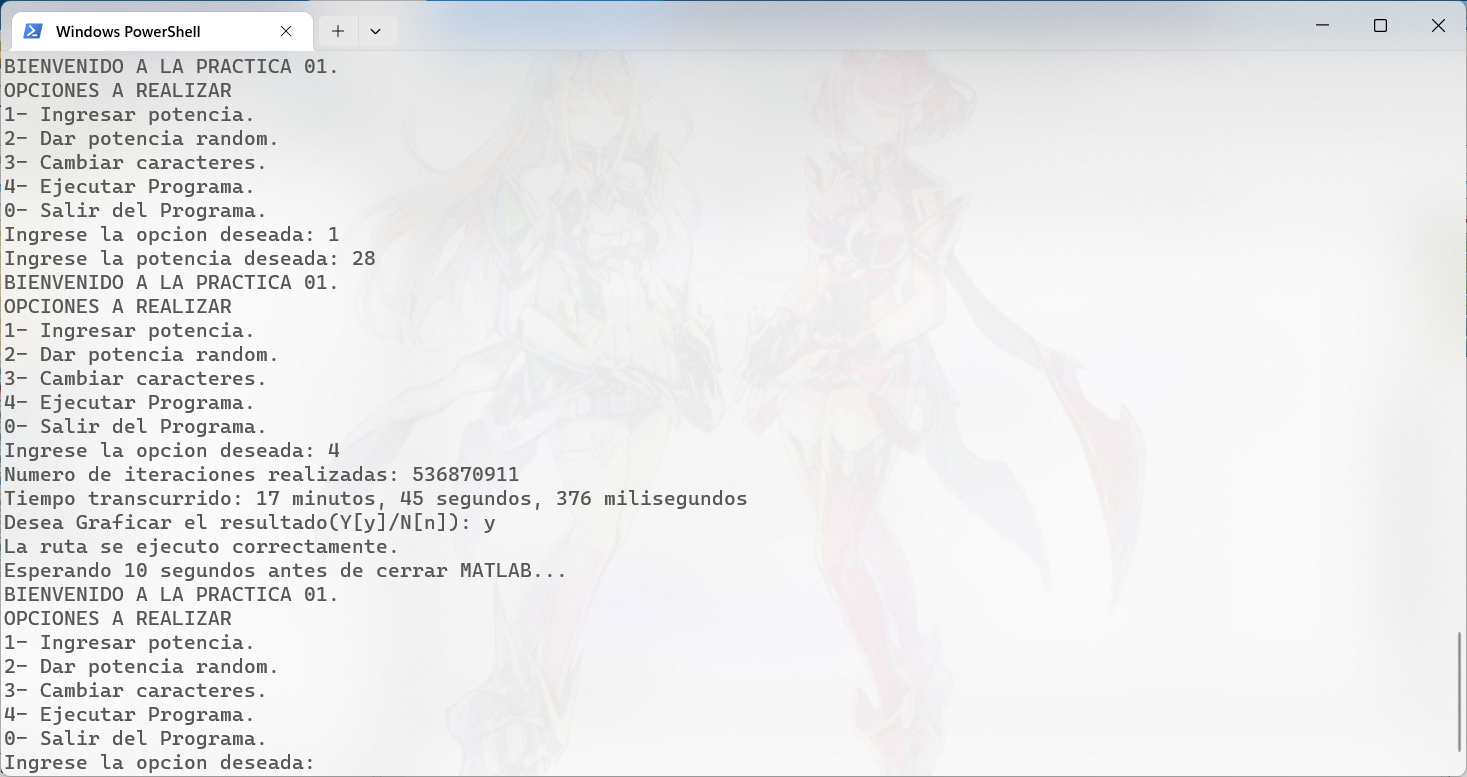
\includegraphics[width=0.75\linewidth]{Terminal.png}
        \caption{Ejecucion de la Practica 01 en terminal.}\label{terminal}
    \end{figure}

    \begin{figure}[H]
        \centering
        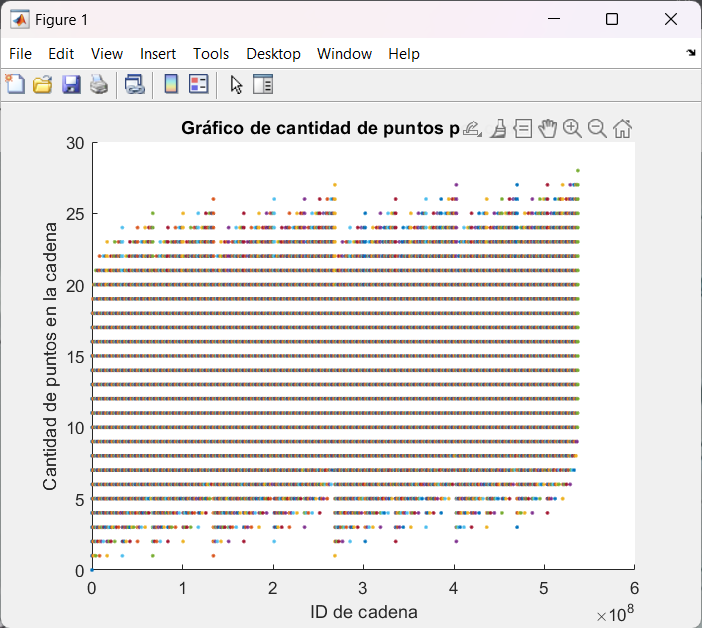
\includegraphics[width=0.6\linewidth]{GraficoPuntos.png}
        \caption{Grafico resultante con potencia = 28}\label{graficaDoble}
    \end{figure}

    Este es el resultado en el \textit{universo.txt} con una potencia igual a cinco:
    \begin{lstlisting}[language={},basicstyle=\ttfamily\footnotesize, breaklines=true]
        e,#,##,###,####,#####,####.,###.,###.#,###..,##.,##.#,##.##,##.#.,##..,
        ##..#,##...,#.,#.#,#.##,#.###,#.##.,#.#.,#.#.#,#.#..,
        #..,#..#,#..##,#..#.,#...,#...#,#....,.,.#,.##,.###,
        .####,.###.,.##.,.##.#,.##..,.#.,.#.#,.#.##,.#.#.,.#..,.#..#,.#...
        ..,..#,..##,..###,..##.,..#.,..#.#,..#..,...,...#,...##,...#.,....,....#,.....
    \end{lstlisting}

    \subsection{Resultados: Tablero de ajedrez}
    A continuación se dejan los resultados dados por el programa con 20 turnos:

    \begin{figure}[H]
        \centering
        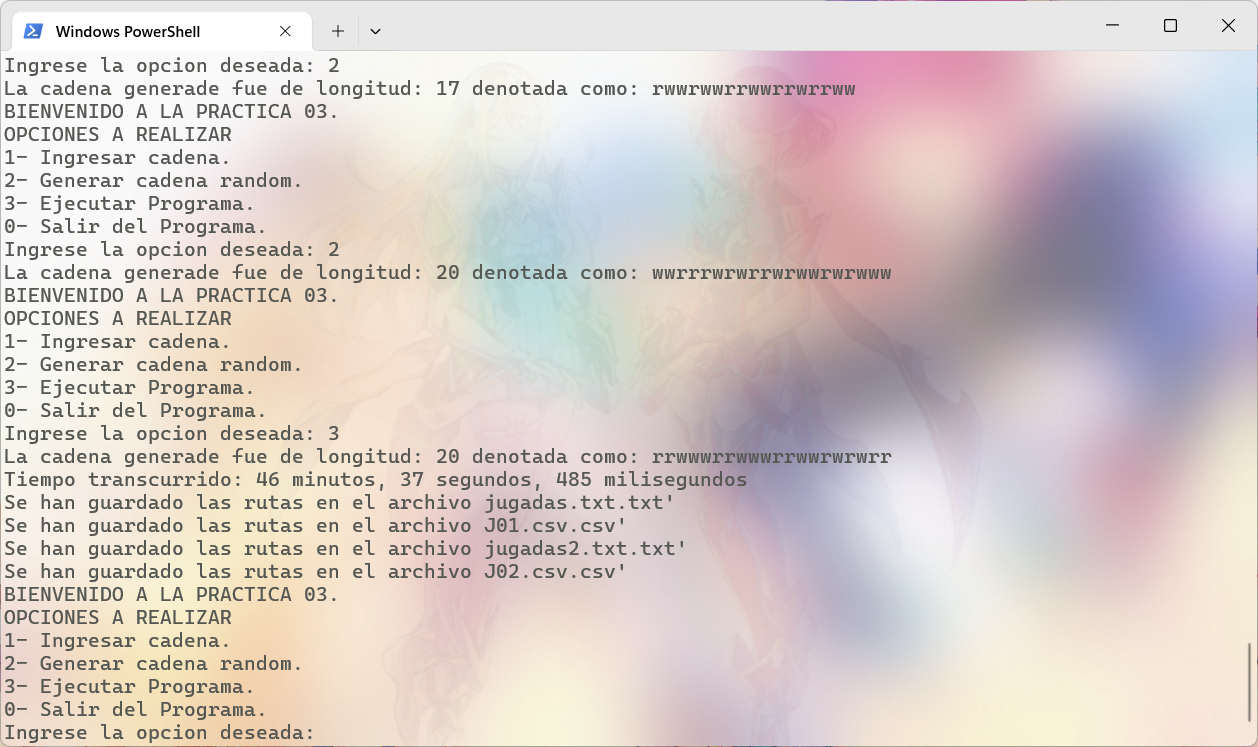
\includegraphics[width=0.75\linewidth]{TerminalP03.png}
        \caption{Ejecucion de la Practica 03 en terminal.}\label{terminalP03}
    \end{figure}

    \begin{figure}[H]
        \centering
        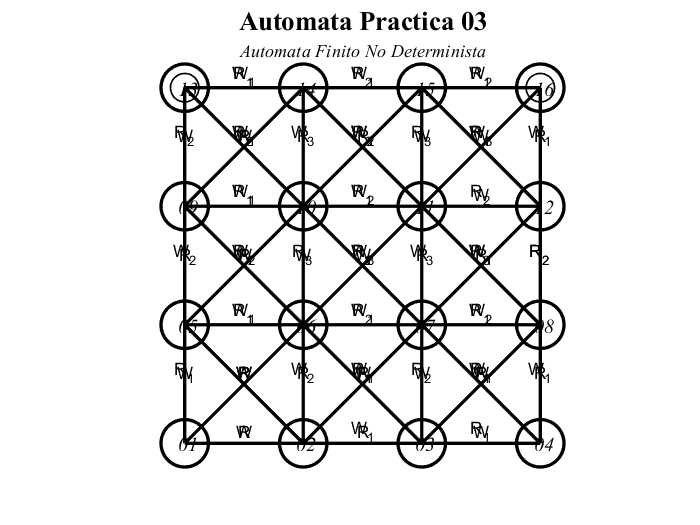
\includegraphics[width=0.6\linewidth]{automataP03.png}
        \caption{Automata Resultante P04}\label{automataP03}
    \end{figure}

    \begin{figure}[H]
        \centering
        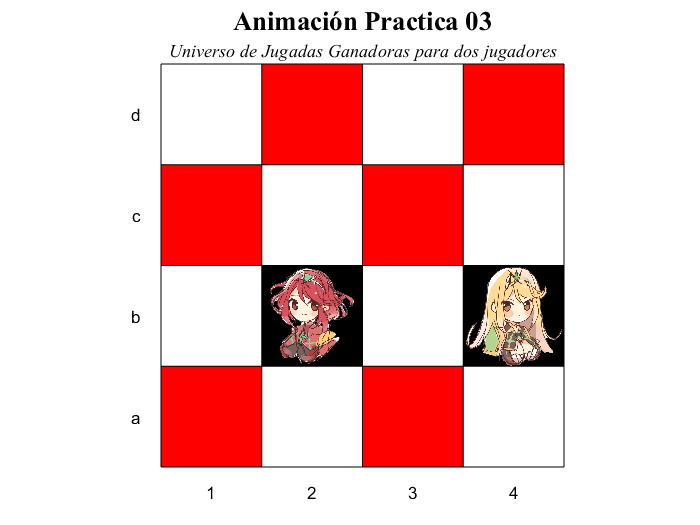
\includegraphics[width=0.6\linewidth]{tablero.png}
        \caption{Tablero de ajedrez}\label{tablero}
    \end{figure}

    Estas son las primeras cincuenta rutas dentro del archivo \textit{jugadas.txt} con una la cadena <<wwwwrrwwrrwwrrw>>,
    el total de rutas es: 253435 (contando desde 1);
    \begin{lstlisting}[language={},basicstyle=\ttfamily\footnotesize, breaklines=true]
Se encontraron las siguientes jugadas para la cadea <<wwwwrrwwrrwwrrw>>:
Ruta: Q0 -> Q5 -> Q0 -> Q5 -> Q0 -> Q1 -> Q4 -> Q0 -> Q5 -> Q1 -> Q4 -> Q0 -> Q5 -> Q6 -> Q11 -> Q15
Ruta: Q0 -> Q5 -> Q0 -> Q5 -> Q0 -> Q1 -> Q4 -> Q0 -> Q5 -> Q1 -> Q4 -> Q0 -> Q5 -> Q9 -> Q14 -> Q15
Ruta: Q0 -> Q5 -> Q0 -> Q5 -> Q0 -> Q1 -> Q4 -> Q0 -> Q5 -> Q1 -> Q4 -> Q5 -> Q2 -> Q6 -> Q11 -> Q15
Ruta: Q0 -> Q5 -> Q0 -> Q5 -> Q0 -> Q1 -> Q4 -> Q0 -> Q5 -> Q1 -> Q4 -> Q5 -> Q8 -> Q9 -> Q14 -> Q15
Ruta: Q0 -> Q5 -> Q0 -> Q5 -> Q0 -> Q1 -> Q4 -> Q0 -> Q5 -> Q1 -> Q4 -> Q5 -> Q10 -> Q6 -> Q11 -> Q15
Ruta: Q0 -> Q5 -> Q0 -> Q5 -> Q0 -> Q1 -> Q4 -> Q0 -> Q5 -> Q1 -> Q4 -> Q5 -> Q10 -> Q9 -> Q14 -> Q15
Ruta: Q0 -> Q5 -> Q0 -> Q5 -> Q0 -> Q1 -> Q4 -> Q0 -> Q5 -> Q1 -> Q4 -> Q5 -> Q10 -> Q11 -> Q14 -> Q15
Ruta: Q0 -> Q5 -> Q0 -> Q5 -> Q0 -> Q1 -> Q4 -> Q0 -> Q5 -> Q1 -> Q4 -> Q5 -> Q10 -> Q14 -> Q11 -> Q15
Ruta: Q0 -> Q5 -> Q0 -> Q5 -> Q0 -> Q1 -> Q4 -> Q0 -> Q5 -> Q1 -> Q4 -> Q8 -> Q5 -> Q6 -> Q11 -> Q15
Ruta: Q0 -> Q5 -> Q0 -> Q5 -> Q0 -> Q1 -> Q4 -> Q0 -> Q5 -> Q1 -> Q4 -> Q8 -> Q5 -> Q9 -> Q14 -> Q15
Ruta: Q0 -> Q5 -> Q0 -> Q5 -> Q0 -> Q1 -> Q4 -> Q0 -> Q5 -> Q1 -> Q4 -> Q8 -> Q13 -> Q9 -> Q14 -> Q15
Ruta: Q0 -> Q5 -> Q0 -> Q5 -> Q0 -> Q1 -> Q4 -> Q0 -> Q5 -> Q1 -> Q4 -> Q8 -> Q13 -> Q14 -> Q11 -> Q15
Ruta: Q0 -> Q5 -> Q0 -> Q5 -> Q0 -> Q1 -> Q4 -> Q0 -> Q5 -> Q1 -> Q6 -> Q2 -> Q5 -> Q6 -> Q11 -> Q15
Ruta: Q0 -> Q5 -> Q0 -> Q5 -> Q0 -> Q1 -> Q4 -> Q0 -> Q5 -> Q1 -> Q6 -> Q2 -> Q5 -> Q9 -> Q14 -> Q15
Ruta: Q0 -> Q5 -> Q0 -> Q5 -> Q0 -> Q1 -> Q4 -> Q0 -> Q5 -> Q1 -> Q6 -> Q2 -> Q7 -> Q6 -> Q11 -> Q15
Ruta: Q0 -> Q5 -> Q0 -> Q5 -> Q0 -> Q1 -> Q4 -> Q0 -> Q5 -> Q1 -> Q6 -> Q2 -> Q7 -> Q11 -> Q14 -> Q15
Ruta: Q0 -> Q5 -> Q0 -> Q5 -> Q0 -> Q1 -> Q4 -> Q0 -> Q5 -> Q1 -> Q6 -> Q5 -> Q2 -> Q6 -> Q11 -> Q15
Ruta: Q0 -> Q5 -> Q0 -> Q5 -> Q0 -> Q1 -> Q4 -> Q0 -> Q5 -> Q1 -> Q6 -> Q5 -> Q8 -> Q9 -> Q14 -> Q15
Ruta: Q0 -> Q5 -> Q0 -> Q5 -> Q0 -> Q1 -> Q4 -> Q0 -> Q5 -> Q1 -> Q6 -> Q5 -> Q10 -> Q6 -> Q11 -> Q15
Ruta: Q0 -> Q5 -> Q0 -> Q5 -> Q0 -> Q1 -> Q4 -> Q0 -> Q5 -> Q1 -> Q6 -> Q5 -> Q10 -> Q9 -> Q14 -> Q15
Ruta: Q0 -> Q5 -> Q0 -> Q5 -> Q0 -> Q1 -> Q4 -> Q0 -> Q5 -> Q1 -> Q6 -> Q5 -> Q10 -> Q11 -> Q14 -> Q15
Ruta: Q0 -> Q5 -> Q0 -> Q5 -> Q0 -> Q1 -> Q4 -> Q0 -> Q5 -> Q1 -> Q6 -> Q5 -> Q10 -> Q14 -> Q11 -> Q15
Ruta: Q0 -> Q5 -> Q0 -> Q5 -> Q0 -> Q1 -> Q4 -> Q0 -> Q5 -> Q1 -> Q6 -> Q7 -> Q2 -> Q6 -> Q11 -> Q15
Ruta: Q0 -> Q5 -> Q0 -> Q5 -> Q0 -> Q1 -> Q4 -> Q0 -> Q5 -> Q1 -> Q6 -> Q7 -> Q10 -> Q6 -> Q11 -> Q15
Ruta: Q0 -> Q5 -> Q0 -> Q5 -> Q0 -> Q1 -> Q4 -> Q0 -> Q5 -> Q1 -> Q6 -> Q7 -> Q10 -> Q9 -> Q14 -> Q15
Ruta: Q0 -> Q5 -> Q0 -> Q5 -> Q0 -> Q1 -> Q4 -> Q0 -> Q5 -> Q1 -> Q6 -> Q7 -> Q10 -> Q11 -> Q14 -> Q15
Ruta: Q0 -> Q5 -> Q0 -> Q5 -> Q0 -> Q1 -> Q4 -> Q0 -> Q5 -> Q1 -> Q6 -> Q7 -> Q10 -> Q14 -> Q11 -> Q15
Ruta: Q0 -> Q5 -> Q0 -> Q5 -> Q0 -> Q1 -> Q4 -> Q0 -> Q5 -> Q1 -> Q6 -> Q10 -> Q5 -> Q6 -> Q11 -> Q15
Ruta: Q0 -> Q5 -> Q0 -> Q5 -> Q0 -> Q1 -> Q4 -> Q0 -> Q5 -> Q1 -> Q6 -> Q10 -> Q5 -> Q9 -> Q14 -> Q15
Ruta: Q0 -> Q5 -> Q0 -> Q5 -> Q0 -> Q1 -> Q4 -> Q0 -> Q5 -> Q1 -> Q6 -> Q10 -> Q7 -> Q6 -> Q11 -> Q15
Ruta: Q0 -> Q5 -> Q0 -> Q5 -> Q0 -> Q1 -> Q4 -> Q0 -> Q5 -> Q1 -> Q6 -> Q10 -> Q7 -> Q11 -> Q14 -> Q15
Ruta: Q0 -> Q5 -> Q0 -> Q5 -> Q0 -> Q1 -> Q4 -> Q0 -> Q5 -> Q1 -> Q6 -> Q10 -> Q13 -> Q9 -> Q14 -> Q15
Ruta: Q0 -> Q5 -> Q0 -> Q5 -> Q0 -> Q1 -> Q4 -> Q0 -> Q5 -> Q1 -> Q6 -> Q10 -> Q13 -> Q14 -> Q11 -> Q15
Ruta: Q0 -> Q5 -> Q0 -> Q5 -> Q0 -> Q1 -> Q4 -> Q0 -> Q5 -> Q1 -> Q6 -> Q10 -> Q15 -> Q11 -> Q14 -> Q15
Ruta: Q0 -> Q5 -> Q0 -> Q5 -> Q0 -> Q1 -> Q4 -> Q0 -> Q5 -> Q1 -> Q6 -> Q10 -> Q15 -> Q14 -> Q11 -> Q15
Ruta: Q0 -> Q5 -> Q0 -> Q5 -> Q0 -> Q1 -> Q4 -> Q0 -> Q5 -> Q4 -> Q1 -> Q0 -> Q5 -> Q6 -> Q11 -> Q15
Ruta: Q0 -> Q5 -> Q0 -> Q5 -> Q0 -> Q1 -> Q4 -> Q0 -> Q5 -> Q4 -> Q1 -> Q0 -> Q5 -> Q9 -> Q14 -> Q15
Ruta: Q0 -> Q5 -> Q0 -> Q5 -> Q0 -> Q1 -> Q4 -> Q0 -> Q5 -> Q4 -> Q1 -> Q2 -> Q5 -> Q6 -> Q11 -> Q15
Ruta: Q0 -> Q5 -> Q0 -> Q5 -> Q0 -> Q1 -> Q4 -> Q0 -> Q5 -> Q4 -> Q1 -> Q2 -> Q5 -> Q9 -> Q14 -> Q15
Ruta: Q0 -> Q5 -> Q0 -> Q5 -> Q0 -> Q1 -> Q4 -> Q0 -> Q5 -> Q4 -> Q1 -> Q2 -> Q7 -> Q6 -> Q11 -> Q15
Ruta: Q0 -> Q5 -> Q0 -> Q5 -> Q0 -> Q1 -> Q4 -> Q0 -> Q5 -> Q4 -> Q1 -> Q2 -> Q7 -> Q11 -> Q14 -> Q15
Ruta: Q0 -> Q5 -> Q0 -> Q5 -> Q0 -> Q1 -> Q4 -> Q0 -> Q5 -> Q4 -> Q1 -> Q5 -> Q2 -> Q6 -> Q11 -> Q15
Ruta: Q0 -> Q5 -> Q0 -> Q5 -> Q0 -> Q1 -> Q4 -> Q0 -> Q5 -> Q4 -> Q1 -> Q5 -> Q8 -> Q9 -> Q14 -> Q15
Ruta: Q0 -> Q5 -> Q0 -> Q5 -> Q0 -> Q1 -> Q4 -> Q0 -> Q5 -> Q4 -> Q1 -> Q5 -> Q10 -> Q6 -> Q11 -> Q15
Ruta: Q0 -> Q5 -> Q0 -> Q5 -> Q0 -> Q1 -> Q4 -> Q0 -> Q5 -> Q4 -> Q1 -> Q5 -> Q10 -> Q9 -> Q14 -> Q15
Ruta: Q0 -> Q5 -> Q0 -> Q5 -> Q0 -> Q1 -> Q4 -> Q0 -> Q5 -> Q4 -> Q1 -> Q5 -> Q10 -> Q11 -> Q14 -> Q15
Ruta: Q0 -> Q5 -> Q0 -> Q5 -> Q0 -> Q1 -> Q4 -> Q0 -> Q5 -> Q4 -> Q1 -> Q5 -> Q10 -> Q14 -> Q11 -> Q15
Ruta: Q0 -> Q5 -> Q0 -> Q5 -> Q0 -> Q1 -> Q4 -> Q0 -> Q5 -> Q4 -> Q9 -> Q5 -> Q2 -> Q6 -> Q11 -> Q15
Ruta: Q0 -> Q5 -> Q0 -> Q5 -> Q0 -> Q1 -> Q4 -> Q0 -> Q5 -> Q4 -> Q9 -> Q5 -> Q8 -> Q9 -> Q14 -> Q15
    \end{lstlisting}
    \subsection{Resultados: Buscador de palabras}
    La tabla de estados del automata DFA resultante fue:
    \begin{table}[!htbp]
        \centering
        \begin{adjustbox}{max width=\textwidth}
        \begin{tabular}{|l|l|l|l|l|l|l|l|l|l|l|l|l|l|l|l|l|l|}
        \hline
            ESTADOS & E & S & C & U & L & A & T & D & I & N & R & O & F & M & Z & ~ & E.F \\ \hline
            0 & 1 & 0 & 28 & 0 & 0 & 0 & 0 & 0 & 0 & 0 & 17 & 0 & 0 & 34 & 0 & 0 & 0 \\ \hline
            1 & 1 & 2 & 28 & 0 & 0 & 0 & 0 & 0 & 0 & 0 & 17 & 0 & 0 & 34 & 0 & 0 & 0 \\ \hline
            2 & 1 & 0 & 3 & 0 & 0 & 0 & 8 & 0 & 0 & 0 & 17 & 0 & 0 & 34 & 0 & 0 & 0 \\ \hline
            3 & 1 & 0 & 28 & 4 & 0 & 0 & 0 & 0 & 0 & 0 & 17 & 0 & 0 & 34 & 0 & 0 & 0 \\ \hline
            4 & 5 & 0 & 28 & 0 & 0 & 0 & 0 & 0 & 0 & 0 & 17 & 0 & 0 & 34 & 0 & 0 & 0 \\ \hline
            5 & 1 & 0 & 28 & 0 & 6 & 0 & 0 & 0 & 0 & 0 & 17 & 0 & 0 & 34 & 0 & 0 & 0 \\ \hline
            6 & 1 & 0 & 28 & 0 & 0 & 7 & 0 & 0 & 0 & 0 & 17 & 0 & 0 & 34 & 0 & 0 & 0 \\ \hline
            7 & 1 & 0 & 28 & 0 & 0 & 0 & 0 & 0 & 0 & 0 & 17 & 0 & 0 & 34 & 0 & 0 & 1 \\ \hline
            8 & 1 & 0 & 28 & 9 & 0 & 0 & 0 & 0 & 0 & 0 & 17 & 0 & 0 & 34 & 0 & 0 & 0 \\ \hline
            9 & 1 & 0 & 28 & 0 & 0 & 0 & 0 & 10 & 0 & 0 & 17 & 0 & 0 & 34 & 0 & 0 & 0 \\ \hline
            10 & 1 & 0 & 28 & 0 & 0 & 0 & 0 & 0 & 11 & 0 & 17 & 0 & 0 & 34 & 0 & 0 & 0 \\ \hline
            11 & 1 & 0 & 28 & 0 & 0 & 12 & 0 & 0 & 0 & 0 & 17 & 0 & 0 & 34 & 0 & 0 & 0 \\ \hline
            12 & 1 & 0 & 28 & 0 & 0 & 0 & 0 & 0 & 0 & 13 & 17 & 0 & 0 & 34 & 0 & 0 & 0 \\ \hline
            13 & 1 & 0 & 28 & 0 & 0 & 0 & 14 & 0 & 0 & 0 & 17 & 0 & 0 & 34 & 0 & 0 & 0 \\ \hline
            14 & 15 & 0 & 28 & 0 & 0 & 0 & 0 & 0 & 0 & 0 & 17 & 0 & 0 & 34 & 0 & 0 & 0 \\ \hline
            15 & 1 & 16 & 28 & 0 & 0 & 0 & 0 & 0 & 0 & 0 & 17 & 0 & 0 & 34 & 0 & 0 & 0 \\ \hline
            16 & 1 & 0 & 3 & 0 & 0 & 0 & 8 & 0 & 0 & 0 & 17 & 0 & 0 & 34 & 0 & 0 & 1 \\ \hline
            17 & 18 & 0 & 28 & 0 & 0 & 0 & 0 & 0 & 23 & 0 & 17 & 0 & 0 & 34 & 0 & 0 & 0 \\ \hline
            18 & 1 & 0 & 28 & 0 & 0 & 0 & 0 & 0 & 0 & 19 & 17 & 0 & 0 & 34 & 0 & 0 & 0 \\ \hline
            19 & 1 & 0 & 20 & 0 & 0 & 0 & 0 & 0 & 0 & 0 & 17 & 0 & 0 & 34 & 0 & 0 & 0 \\ \hline
            20 & 1 & 0 & 28 & 0 & 0 & 0 & 0 & 0 & 0 & 0 & 17 & 21 & 0 & 34 & 0 & 0 & 0 \\ \hline
            21 & 1 & 0 & 28 & 0 & 0 & 0 & 0 & 0 & 0 & 0 & 22 & 0 & 0 & 34 & 0 & 0 & 0 \\ \hline
            22 & 18 & 0 & 28 & 0 & 0 & 0 & 0 & 0 & 23 & 0 & 17 & 0 & 0 & 34 & 0 & 0 & 1 \\ \hline
            23 & 1 & 0 & 28 & 0 & 0 & 0 & 0 & 0 & 0 & 0 & 17 & 0 & 24 & 34 & 0 & 0 & 0 \\ \hline
            24 & 1 & 0 & 28 & 0 & 25 & 0 & 0 & 0 & 0 & 0 & 17 & 0 & 0 & 34 & 0 & 0 & 0 \\ \hline
            25 & 26 & 0 & 28 & 0 & 0 & 0 & 0 & 0 & 0 & 0 & 17 & 0 & 0 & 34 & 0 & 0 & 0 \\ \hline
            26 & 1 & 27 & 28 & 0 & 0 & 0 & 0 & 0 & 0 & 0 & 17 & 0 & 0 & 34 & 0 & 0 & 0 \\ \hline
            27 & 1 & 0 & 3 & 0 & 0 & 0 & 8 & 0 & 0 & 0 & 17 & 0 & 0 & 34 & 0 & 0 & 1 \\ \hline
            28 & 1 & 0 & 28 & 0 & 0 & 0 & 0 & 0 & 0 & 0 & 29 & 0 & 0 & 34 & 0 & 0 & 0 \\ \hline
            29 & 1 & 0 & 28 & 0 & 0 & 0 & 0 & 0 & 30 & 0 & 17 & 0 & 0 & 34 & 0 & 0 & 0 \\ \hline
            30 & 1 & 0 & 28 & 0 & 0 & 0 & 0 & 0 & 0 & 0 & 17 & 0 & 0 & 31 & 0 & 0 & 0 \\ \hline
            31 & 32 & 0 & 28 & 0 & 0 & 0 & 0 & 0 & 0 & 0 & 17 & 0 & 0 & 34 & 0 & 0 & 0 \\ \hline
            32 & 1 & 0 & 28 & 0 & 0 & 0 & 0 & 0 & 0 & 33 & 17 & 0 & 0 & 34 & 0 & 0 & 0 \\ \hline
            33 & 1 & 0 & 28 & 0 & 0 & 0 & 0 & 0 & 0 & 0 & 17 & 0 & 0 & 34 & 0 & 0 & 1 \\ \hline
            34 & 1 & 0 & 28 & 0 & 0 & 35 & 0 & 0 & 0 & 0 & 17 & 0 & 0 & 34 & 0 & 0 & 0 \\ \hline
            35 & 1 & 0 & 28 & 0 & 0 & 0 & 36 & 0 & 0 & 0 & 17 & 0 & 0 & 34 & 0 & 0 & 0 \\ \hline
            36 & 1 & 0 & 28 & 0 & 0 & 37 & 0 & 0 & 0 & 0 & 17 & 0 & 0 & 34 & 0 & 0 & 0 \\ \hline
            37 & 1 & 0 & 28 & 0 & 0 & 0 & 0 & 0 & 0 & 38 & 17 & 0 & 0 & 34 & 0 & 0 & 0 \\ \hline
            38 & 1 & 0 & 28 & 0 & 0 & 0 & 0 & 0 & 0 & 0 & 17 & 0 & 0 & 34 & 39 & 0 & 0 \\ \hline
            39 & 1 & 0 & 28 & 0 & 0 & 40 & 0 & 0 & 0 & 0 & 17 & 0 & 0 & 34 & 0 & 0 & 0 \\ \hline
            40 & 1 & 0 & 28 & 0 & 0 & 0 & 0 & 0 & 0 & 0 & 17 & 0 & 0 & 34 & 0 & 0 & 1 \\ \hline
        \end{tabular}
        \end{adjustbox}
        \caption{Tabla de Estados del DFA}
    \end{table}
    \newpage
    A continuación se dejan los resultados dados por el programa con el url:
    <<\href{https://mvsnoticias.com/nacional/2024/4/2/investigar-morena-por-presunto-financiamiento-del-crimen-sus-campanas-oposicion-633307.html}{Noticia}>>:

    \begin{figure}[H]
        \centering
        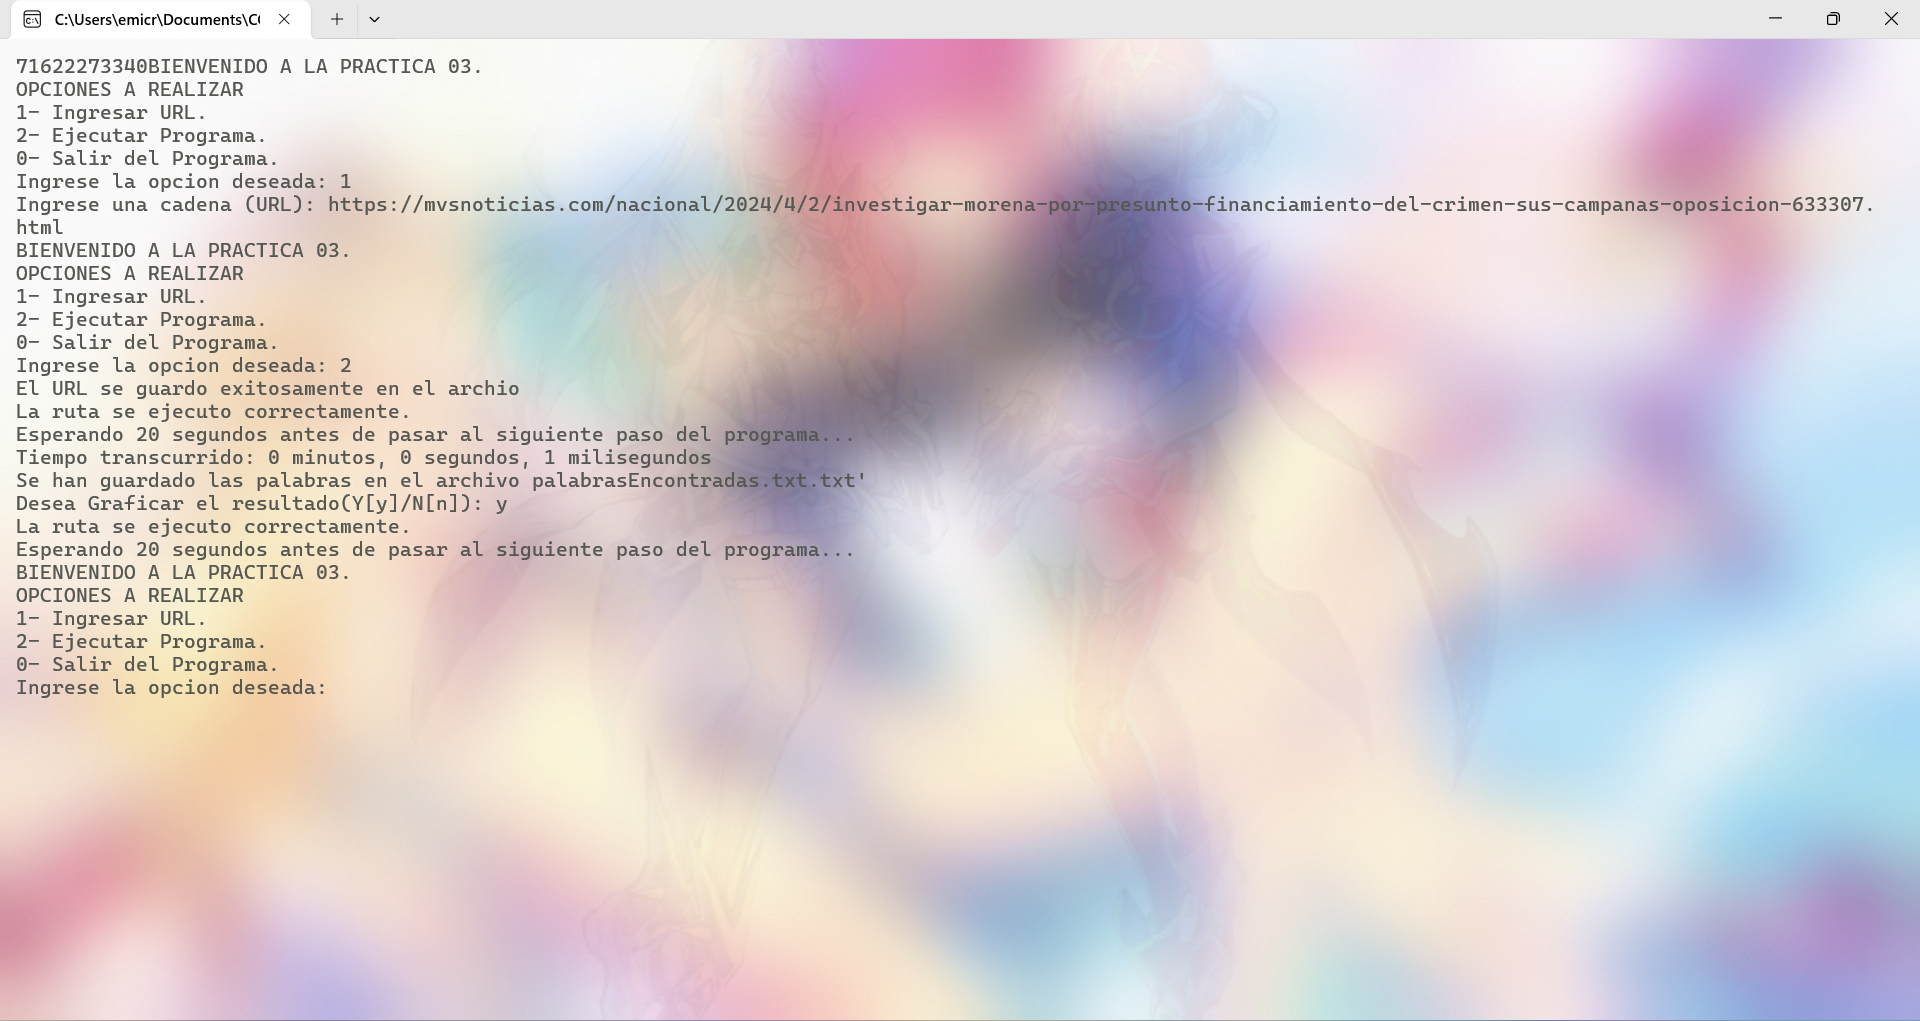
\includegraphics[width=0.75\linewidth]{TerminalP04.png}
        \caption{Ejecucion de la Practica 04 en terminal.}\label{terminalP04}
    \end{figure}

    \begin{figure}[H]
        \centering
        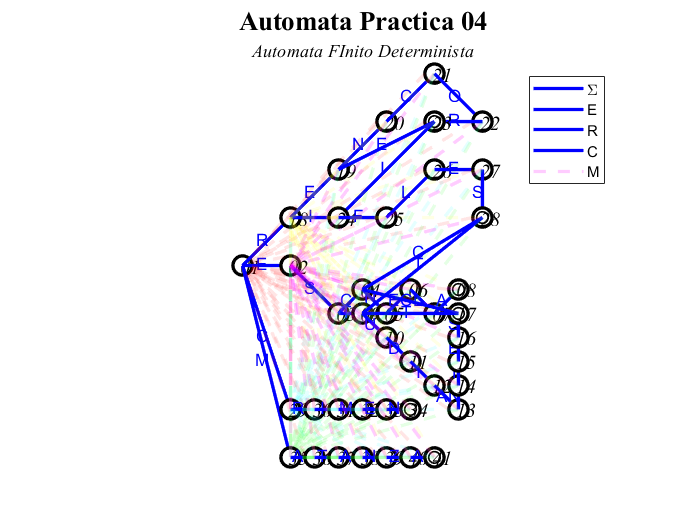
\includegraphics[width=0.6\linewidth]{automataP04.png}
        \caption{Automata Resultante P04}\label{automataP04}
    \end{figure}

    \begin{lstlisting}[language={},basicstyle=\ttfamily\footnotesize, breaklines=true]
Palabra: crimen	Coordenada en X: 287	Coordenada en Y: 11
Palabra: crimen	Coordenada en X: 63	Coordenada en Y: 29
Palabra: crimen	Coordenada en X: 52	Coordenada en Y: 33
Palabra: crimen	Coordenada en X: 209	Coordenada en Y: 35
Palabra: crimen	Coordenada en X: 32	Coordenada en Y: 41
Palabra: crimen,	Coordenada en X: 127	Coordenada en Y: 41
    \end{lstlisting}
\newpage
\section{Conclusiones}
Durante esta actividad, se desarrollaron tres programas distintos: \textit{Universo}, \textit{Tablero} y \textit{Buscador de Palabras},
cada uno con sus propias características y desafíos. La combinación de lenguajes de programación como C++ y MATLAB permitió abordar
eficazmente cada uno de estos problemas, ofreciendo soluciones robustas y eficientes.

Con el programa \textit{Universo}, se exploró la generación y manipulación de cadenas binarias de longitud variable, demostrando la
versatilidad y eficiencia de C++ en el manejo de grandes conjuntos de datos. La capacidad de MATLAB para visualizar estos datos
facilitó la comprensión y el análisis de los resultados obtenidos.

El programa \textit{Tablero} abordó la simulación de movimientos en un tablero de ajedrez, incorporando reglas de juego y condiciones
de victoria. La flexibilidad de C++ y la capacidad de MATLAB para graficar y visualizar datos permitieron crear una solución completa
que puede ejecutarse tanto de forma automática como manual.

Por último, el desarrollo del \textit{Buscador de Palabras} se centró en la implementación de un autómata capaz de reconocer un
conjunto específico de palabras. Esta aplicación demostró la eficacia de los autómatas en el procesamiento de texto y la utilidad de
la combinación de C++ y MATLAB para implementar soluciones complejas.

En conclusión, la combinación de estos lenguajes proporcionó una solución integral para diseñar, implementar y analizar los programas
desarrollados en esta actividad, ofreciendo resultados satisfactorios y cumpliendo con los requisitos establecidos.

\bibliographystyle{ieeetr}
\newpage
\bibliography{referencias}

\end{document}
